% !TeX encoding = UTF-8
% Chuyển từ: C:\Users\ADMIN\Documents\NCKH\Repo\Bản chuẩn.docx
% Biên dịch bằng XeLaTeX hoặc LuaLaTeX.
% Giữ nội dung bản Word; hình minh họa được để chỗ trống để bổ sung sau.
\documentclass[12pt,a4paper,oneside]{report}

\usepackage{fontspec}
\IfFontExistsTF{Times New Roman}{%
  \setmainfont{Times New Roman}%
}{%
  \setmainfont{TeX Gyre Termes}%
}
\usepackage[left=3cm,right=2cm,top=2.5cm,bottom=2.5cm]{geometry}
\usepackage{amsmath,amssymb}
\usepackage{graphicx}
\usepackage{booktabs,array}
\usepackage{pdflscape}
\usepackage{enumitem}
\usepackage{setspace}
\usepackage{titlesec}
\usepackage[unicode,hidelinks]{hyperref}

\renewcommand{\chaptername}{Chương}
\renewcommand{\contentsname}{Mục lục}
\renewcommand{\listfigurename}{Danh mục hình ảnh}
\renewcommand{\figurename}{Hình}
\renewcommand{\tablename}{Bảng}
\renewcommand{\bibname}{Tài liệu tham khảo}
\setcounter{secnumdepth}{2}
\setcounter{tocdepth}{2}
\setlength{\parindent}{1cm}
\setlength{\parskip}{4pt}
\setlength{\emergencystretch}{3em}
\setlist[itemize]{leftmargin=*,itemsep=3pt,topsep=4pt}
\onehalfspacing
\graphicspath{{picture/}}

% Chú thích chuẩn cho hình đặt cố định, đồng thời ghi vào danh mục hình.
\makeatletter
\newcommand{\chuthichhinh}[2][]{%
  \begingroup
    \def\@captype{figure}%
    \caption{#2}%
    \if\relax\detokenize{#1}\relax\else\label{#1}\fi
  \endgroup
}
\makeatother

% Khung chờ: đối số tùy chọn là tên ngắn dùng cho chú thích và danh mục.
\newcommand{\hinhminhhoa}[2][]{%
  \begin{center}
    \begin{minipage}{\linewidth}
    \centering
    \fbox{\parbox[c][4cm][c]{0.9\linewidth}{\centering
      #2\\[4pt]
      \textit{(Bổ sung hình ảnh sau)}
    }}
    \if\relax\detokenize{#1}\relax
      \chuthichhinh{#2}%
    \else
      \chuthichhinh{#1}%
    \fi
    \end{minipage}
  \end{center}
}

\titleformat{\chapter}[display]
  {\normalfont\bfseries\centering\Large}
  {\MakeUppercase{\chaptername}\ \thechapter}{8pt}{\Large}
\titlespacing*{\chapter}{0pt}{0pt}{18pt}
\titleformat{\section}{\normalfont\large\bfseries}{\thesection.}{0.5em}{}
\titleformat{\subsection}{\normalfont\normalsize\bfseries}{\thesubsection.}{0.5em}{}

\begin{document}

\pagenumbering{roman}
\tableofcontents
\clearpage
\phantomsection
\addcontentsline{toc}{chapter}{\listfigurename}
\listoffigures
\clearpage
\pagenumbering{arabic}

\chapter{TỔNG QUAN VỀ ĐỀ TÀI VÀ HỆ THỐNG HÓA CÁC DẠNG BÀI TOÁN QUY HOẠCH QUỸ ĐẠO}

\section{Đặt vấn đề và Tính cấp thiết của đề tài}

\subsection{Bối cảnh phát triển của robot di động và xe tự hành (AMR/AGV) trong công nghiệp và logistics.}

\subsubsection*{a. Trong nước}

Tại Việt Nam, nghiên cứu về AMR/AGV chủ yếu tập trung vào mô hình thử nghiệm nhỏ phục vụ nhà xưởng, kho bãi hoặc phòng lab. Các công trình đã bước đầu ứng dụng các thuật toán (A*, Dijkstra, APF) kết hợp với các cảm biến. Tuy nhiên, mới dừng lại ở mức mô phỏng.

\subsubsection*{b. Ngoài nước}

Trên thế giới, AMR/AGV phát triển vượt bậc và ứng dụng sâu trong logistics, nhà máy thông minh và xe tự hành. Nghiên cứu quốc tế không chỉ tìm đường mà còn tối ưu độ trơn, thời gian tính toán và né vật cản động thời gian thực. Xu hướng tập trung vào các giải thuật lai, tối ưu hóa nâng cao, điều khiển dự báo kết hợp AI.

\subsection{Vai trò của tầng quy hoạch quỹ đạo trong kiến trúc điều khiển tự hành tổng thể (Sense – Plan – Act).}

Trong khoa học robot và các hệ thống điều khiển tự hành, kiến trúc cổ điển Sense--Plan--Act (SPA) đóng vai trò là khung mẫu chuẩn mực mô tả chu trình khép kín từ nhận thức môi trường đến thực thi hành động vật lý. Trong chu trình này, tầng Quy hoạch quỹ đạo (Trajectory Planning) giữ vị trí trọng yếu thuộc khối Plan, là mắt xích quyết định tính khả thi, sự an toàn và hiệu năng vận hành thực tế của robot.

\subsubsection*{a. Vị trí của quy hoạch quỹ đạo trong chu trình Sense--Plan--Act}

Kiến trúc điều khiển tự hành tổng thể được chia thành ba phân tầng chức năng chính:

% TODO: Thay khung dưới bằng ảnh kiến trúc Sense--Plan--Act.
% Khi có ảnh, thay lệnh \hinhminhhoa bằng:
% \centering\includegraphics[width=0.95\linewidth]{sense-plan-act.png}
\noindent\begin{minipage}{\linewidth}
  \begin{center}
    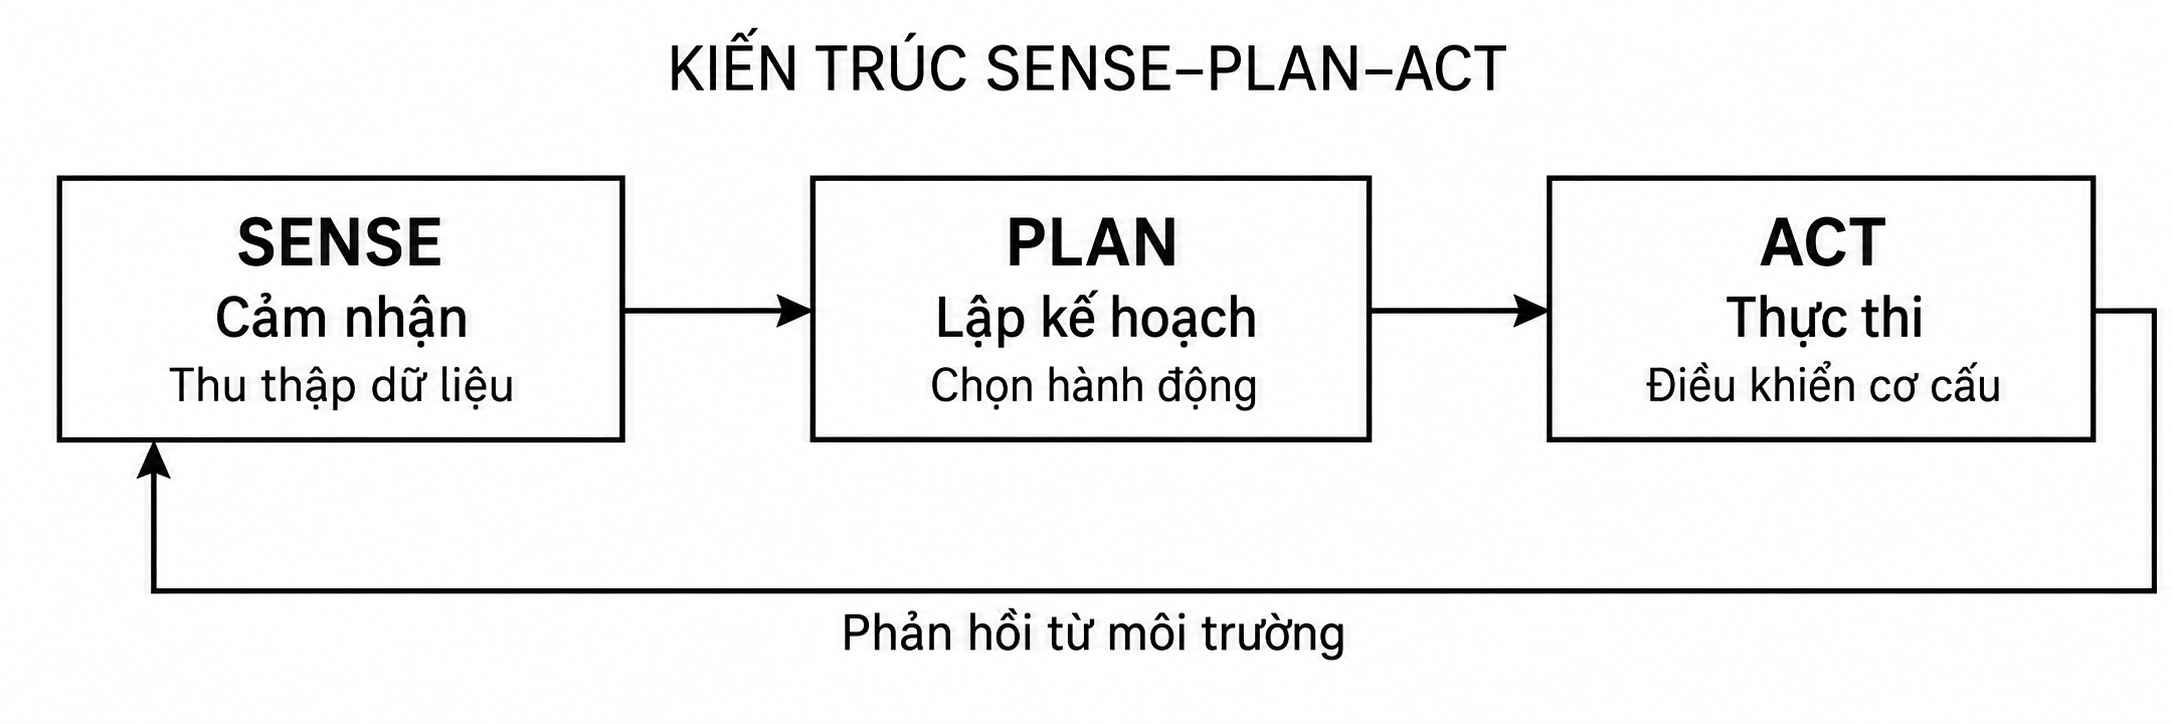
\includegraphics[width=0.95\linewidth]{Kientruc_sense_plan_act.png}
  \end{center}
  \begin{center}
    \chuthichhinh[fig:sense-plan-act]{Các tầng chính của kiến trúc điều khiển tự hành}
  \end{center}
\end{minipage}\par\medskip

\begin{itemize}
  \item \textbf{Khối Sense (Cảm nhận \& Nhận thức):} Thu thập dữ liệu thô từ hệ thống cảm biến như encoder, LiDAR,\ldots{} để thực hiện định vị (Localization), lập bản đồ và xây dựng không gian trạng thái môi trường.
  \item \textbf{Khối Plan (Lập kế hoạch \& Ra quyết định):} Xử lý thông tin từ tầng Sense để chuyển hóa mục tiêu nhiệm vụ thành các chuyển động cụ thể. Tầng này chia thành các cấp:
  \begin{itemize}
    \item \textbf{Task/Mission Planning:} Lập kế hoạch hành vi cấp cao (ví dụ: gắp vật thể, di chuyển đến trạm sạc).
    \item \textbf{Global Path Planning:} Tìm đường đi hình học thô \(C(s)\) từ điểm xuất phát đến đích trên bản đồ tĩnh toàn cục (bỏ hoàn toàn yếu tố thời gian).
    \item \textbf{Trajectory Planning (Local Planning):} Gán biến thời gian \(t\), vận tốc, gia tốc, độ giật và tối ưu hóa chuyển động để tạo thành quỹ đạo động học \(q(t)\) khả thi.
  \end{itemize}
  \item \textbf{Khối Act (Thực thi \& Chấp hành):} Nhận tín hiệu điều khiển tham chiếu từ khối Plan và thực hiện đóng vòng điều khiển (PID, LQR, Torque Controller), cấp xung tới driver động cơ hoặc cơ cấu chấp hành.
\end{itemize}

\subsubsection*{b. Vai trò cốt lõi của tầng quy hoạch quỹ đạo}

\noindent\textbf{Cầu nối giữa quy hoạch nhiệm vụ cấp cao và điều khiển động cơ cấp thấp.}

Quy hoạch quỹ đạo chuyển dịch các mô hình hình học thuần túy (không gian Đề-các hoặc chuỗi điểm nút) thành các chuỗi tín hiệu tham chiếu thời gian thực (Position, Velocity, Acceleration) để các bộ điều khiển cấp thấp có thể bám sát. Không có tầng này, các bộ điều khiển động cơ không thể chấp hành trực tiếp một đường đi hình học do thiếu thông tin về thời gian và giới hạn tốc độ tại từng điểm.

\noindent\textbf{Đảm bảo độ trơn và độ bền cơ khí.}

Bằng cách áp dụng các mô hình nội suy đa thức bậc cao hoặc profile vận tốc dạng chữ S (S-Curve Profile), tầng quy hoạch quỹ đạo loại bỏ các bước nhảy đột ngột của gia tốc (loại bỏ độ giật vô hạn, \(\mathrm{Jerk}=\infty\)).

\subsection{Khảo sát tình hình nghiên cứu trong nước và quốc tế về bài toán quy hoạch quỹ đạo robot.}

\subsubsection*{a. Trong nước}

Ở Việt Nam, bài toán quy hoạch quỹ đạo trong điều khiển robot đã và đang nhận được sự quan tâm trong nhiều đề tài nghiên cứu khoa học, luận văn, đồ án tốt nghiệp và các công trình ứng dụng thuộc các lĩnh vực tự động hóa, cơ điện tử, điều khiển học, trí tuệ nhân tạo và robot học. Các hướng nghiên cứu trong nước thường tập trung vào robot di động, xe tự hành mô hình, robot bám vạch, robot tránh vật cản, robot bám quỹ đạo và robot hoạt động trong môi trường có cấu trúc như phòng thí nghiệm, nhà xưởng hoặc không gian trong nhà. Trong các nghiên cứu này, quy hoạch quỹ đạo giữ vai trò quan trọng nhằm xác định đường đi phù hợp từ vị trí ban đầu đến vị trí đích, đồng thời bảo đảm robot có thể tránh va chạm với vật cản, giảm sai số di chuyển và nâng cao tính ổn định trong quá trình vận hành.

Một số công trình khai thác các thuật toán tìm đường nổi tiếng như Dijkstra, A*, các thuật toán trường thế nhân tạo, các thuật toán bám quỹ đạo Pure Pursuit hoặc các phương pháp điều khiển mở để giải quyết các bài toán theo hướng cho robot di động. Bên cạnh đó, cùng với sự phát triển của xử lý ảnh, các cảm biến siêu âm, LiDAR, encoder hoặc IMU được sử dụng để hỗ trợ robot nhận biết môi trường, xác định vị trí, phát hiện vật cản và hiệu chỉnh quỹ đạo di chuyển. Một số hướng nghiên cứu mới cũng bắt đầu quan tâm đến việc cải thiện thuật toán quy hoạch quỹ đạo nhằm rút ngắn quãng đường đi, giảm thời gian tính toán, làm trơn quỹ đạo và tăng khả năng ứng dụng trong môi trường thực tế.

Tuy nhiên, phần lớn các nghiên cứu trong nước vẫn dừng lại ở mức mô phỏng, mô hình robot quy mô nhỏ hoặc các bài toán thử nghiệm đơn giản. Vì vậy, đề tài nghiên cứu các dạng bài toán quy hoạch quỹ đạo trong điều khiển robot có ý nghĩa thiết thực, góp phần hệ thống hóa cơ sở lý thuyết, phân tích đặc điểm của từng dạng bài toán, mô phỏng các thuật toán tiêu biểu và tạo tiền đề cho việc ứng dụng vào các mô hình robot phục vụ đào tạo và nghiên cứu thực nghiệm tại các trường đại học.

\subsubsection*{b. Ngoài nước}

Trên thế giới, quy hoạch quỹ đạo trong điều khiển robot là một hướng nghiên cứu quan trọng, có tốc độ phát triển nhanh và được ứng dụng rộng rãi trong nhiều lĩnh vực như robot di động, robot công nghiệp, xe tự hành, robot dịch vụ, robot cộng tác, robot nông nghiệp và các hệ thống tự động thông minh. Các nghiên cứu quốc tế hiện nay không chỉ dừng lại ở việc tìm các đường đi từ vị trí ban đầu đến đích, mà còn chú trọng đến nhiều yêu cầu phức tạp hơn như tránh va chạm, tối ưu chiều dài quỹ đạo, giảm thời gian tính toán, bảo đảm độ trơn của đường đi, đáp ứng các ràng buộc động học và động lực học.

Trong lĩnh vực robot di động, các thuật toán quy hoạch đường đi truyền thống như Dijkstra, A*, trường thế nhân tạo, PRM, RRT và các biến thể cải tiến của chúng đã được nghiên cứu rộng rãi nhằm giúp robot xác định quỹ đạo an toàn, hiệu quả trong không gian hai và ba chiều. Nhìn chung, tình hình nghiên cứu ngoài nước cho thấy quy hoạch quỹ đạo robot đang phát triển theo hướng tối ưu hơn, thông minh hơn, chính xác và gần với điều kiện thực tế hơn. Đây là cơ sở quan trọng để nghiên cứu trong nước tham khảo, mô phỏng, so sánh và triển khai phù hợp với điều kiện đào tạo, nghiên cứu tại các trường đại học.

\section{Các Khái niệm Cơ sở trong Quy hoạch Chuyển động}

\subsection{Phân biệt bản chất toán học: Đường đi (Path), Quỹ đạo (Trajectory) và Điều khiển bám (Tracking).}

\subsubsection*{a. Đường đi (Path)}
Path(Đường đi) là tập hợp các điểm trong không gian khớp hoặc không gian hoạt động (không gian làm việc) mà robot đi qua để chuyển từ trạng thái ban đầu đến trạng thái đích mà chưa xét đến yếu tố thời gian, vận tốc hay gia tốc
\subsubsection*{b. Quỹ đạo (Trajectory)}

Trajectory chính là một path đã được gắn thêm quy luật thời gian (timing law). Nói cách khác, trajectory không chỉ trả lời câu hỏi ``robot đi theo hình dạng nào'' mà còn trả lời thêm câu hỏi ``robot đi qua từng điểm đó với vận tốc và gia tốc bao nhiêu, vào thời điểm nào''. Do vậy, trajectory là khái niệm đầy đủ hơn, bao hàm cả thông tin hình học (từ path) lẫn thông tin động học theo thời gian (vận tốc, gia tốc tại mỗi điểm).

% Nội dung được cung cấp chưa có đoạn riêng về Điều khiển bám (Tracking).

\subsection{Không gian Làm việc (Workspace - W) và Không gian Cấu hình (Configuration Space - C - Space).}

Việc lựa chọn không gian biểu diễn quyết định ý nghĩa của một điểm tìm kiếm, cách kiểm tra va chạm và số biến mà thuật toán phải xử lý. Một điểm trên mặt sàn chỉ mô tả vị trí; để xác định đầy đủ robot đang chiếm vùng nào, còn cần biết hướng thân xe và hình học của nó. Do đó, biểu diễn chuyển động trong không gian vật lý và biểu diễn bằng cấu hình có quan hệ chặt chẽ nhưng không thể thay thế tùy ý cho nhau.

\subsubsection*{a. Không gian cấu hình}

\textbf{Định nghĩa:} Cấu hình \(q\) là tập hợp tối thiểu các tọa độ độc lập cần thiết để xác định vị trí của các bộ phận robot khi đã biết các quan hệ hình học của cơ cấu. Tập tất cả cấu hình hợp lệ tạo thành không gian cấu hình \(C\). Số chiều của \(C\) bằng số bậc tự do cấu hình; tuy nhiên, không gian này có thể chứa tọa độ tuần hoàn, giới hạn khớp hoặc ràng buộc liên kết, nên không phải lúc nào cũng đồng nhất với toàn bộ \(\mathbb{R}^{n}\) \cite{lavalle-planning-2006}.

Đối với robot di động được xem là vật rắn trên mặt phẳng, cấu hình thân xe được biểu diễn bởi
\[
  q=(x,y,\theta),\qquad C\simeq SE(2)=\mathbb{R}^{2}\times S^{1}.
\]
Trong đó, \(x,y\) là tọa độ điểm tham chiếu trên thân robot và \(\theta\) là hướng. Ký hiệu \(S^{1}\) thể hiện góc có tính tuần hoàn: \(\theta\) và \(\theta+2\pi\) mô tả cùng một hướng. Khi tính sai lệch hướng, có thể dùng
\[
  \Delta\theta=\operatorname{atan2}
  \bigl(\sin(\theta_2-\theta_1),\cos(\theta_2-\theta_1)\bigr).
\]
Chẳng hạn, hai hướng \(179^{\circ}\) và \(-179^{\circ}\) chỉ cách nhau \(2^{\circ}\) theo cung ngắn, trong khi phép trừ thông thường cho trị tuyệt đối \(358^{\circ}\). Sự khác biệt này ảnh hưởng trực tiếp đến nội suy hướng và lựa chọn nút gần nhất.

Với tay máy phẳng hai khớp quay, có thể chọn \(q=(\theta_1,\theta_2)\). Nếu cả hai khớp quay không giới hạn thì cấu trúc không gian là \(S^{1}\times S^{1}\); nếu có chặn cơ khí, miền tìm kiếm phải thu hẹp theo giới hạn từng khớp. Một điểm trong không gian này xác định tư thế của cả hai khâu, chứ không chỉ vị trí đầu công tác. Hai cấu hình khuỷu trên và khuỷu dưới có thể đưa đầu công tác tới cùng một vị trí nhưng tạo ra hai vùng chiếm chỗ khác nhau.

\textbf{Phân biệt cấu hình và trạng thái:} Cấu hình chưa mô tả đầy đủ khả năng chuyển động trong tương lai khi bài toán có giới hạn gia tốc hoặc lực. Khi đó, cần mở rộng sang trạng thái, chẳng hạn \(z=(q,\dot q)\), hoặc \(z=(x,y,\theta,v,\omega)\) đối với mô hình xe có xét biến thiên vận tốc. Hai robot ở cùng vị trí và cùng hướng nhưng có vận tốc khác nhau sẽ cần khoảng dừng khác nhau. Vì vậy, tìm đường hình học trên \(C\) và quy hoạch có ràng buộc động lực học là hai mức mô hình hóa khác nhau \cite{lavalle-planning-2006}.

\textbf{Vai trò đối với lập kế hoạch chuyển động:} Khi chuyển các vật cản sang không gian cấu hình, toàn bộ robot có thể được đại diện bằng một điểm \(q\). Thuật toán tìm một đường liên tục \(\gamma:[0,1]\to C\), nối \(q_{\mathrm{start}}\) với \(q_{\mathrm{goal}}\), rồi kiểm tra đường này có thuộc miền tự do hay không. Đối với xe phi holonomic, điều kiện đó còn phải kết hợp với ràng buộc vận tốc; một đường liên tục không va chạm vẫn có thể yêu cầu chuyển động ngang mà xe không thực hiện được.

Trong triển khai, khoảng cách giữa các cấu hình phải phản ánh ý nghĩa các tọa độ. Một lựa chọn cho xe phẳng là
\[
  d_C(q_1,q_2)=\sqrt{(x_2-x_1)^2+(y_2-y_1)^2+
       (\ell_{\theta}\Delta\theta)^2},
\]
với \(\ell_{\theta}>0\) là độ dài quy đổi góc sang ảnh hưởng hình học. Đây là một lựa chọn phục vụ tìm kiếm, không phải độ dài đường đi thực tế của mọi loại robot. Giá trị quy đổi cần phù hợp với kích thước thân xe và cách thuật toán nối hai cấu hình.

\subsubsection*{b. Không gian làm việc}

\textbf{Không gian làm việc (Workspace)} \(W\) là không gian vật lý trong đó robot hoạt động, có thể được biểu diễn trong hai hoặc ba chiều tùy theo bài toán. Không gian này bao gồm các vùng trống và các vùng bị chiếm bởi vật cản. Việc mô tả không gian làm việc là cơ sở để xác định vị trí robot, bố trí vật cản và kiểm tra va chạm trong quá trình quy hoạch chuyển động.

Đối với tay máy hai khâu có chiều dài \(l_1,l_2\), ánh xạ động học thuận từ cấu hình sang vị trí đầu công tác là
\[
  p=f(q)=\begin{bmatrix}
    l_1\cos\theta_1+l_2\cos(\theta_1+\theta_2)\\
    l_1\sin\theta_1+l_2\sin(\theta_1+\theta_2)
  \end{bmatrix}.
\]
Nếu bỏ qua vật cản và giới hạn góc khớp, khoảng cách từ gốc tới đầu công tác thỏa mãn \(|l_1-l_2|\leq\|p\|\leq l_1+l_2\). Công thức cho thấy miền với tới phụ thuộc hình học cơ cấu. Khi có vật cản, một vị trí nằm trong miền với tới vẫn có thể không tiếp cận được từ cấu hình xuất phát bằng một chuyển động an toàn.

Với xe di động, một điểm \((x,y)\) nằm giữa hành lang chưa đủ chứng minh xe đi qua được. Cùng một tâm xe nhưng hai góc hướng khác nhau có thể tạo ra một tư thế lọt hành lang và một tư thế chạm tường. Bản đồ 2D vì vậy phải đi kèm mô hình kích thước robot hoặc được chuyển thành bản đồ đã mở rộng vật cản.

\textbf{Ý nghĩa đối với lựa chọn thuật toán:} Bản đồ ô lưới trên \(W\) thuận tiện cho Dijkstra và A*, trong khi các phương pháp lấy mẫu có thể làm việc trực tiếp trên cấu hình nhiều chiều. Nếu mỗi trục được chia thành \(m\) mức, lưới \(n\) chiều có tới \(m^{n}\) tổ hợp. Chẳng hạn, thêm hướng xe với 72 mức góc vào lưới vị trí sẽ làm số trạng thái tiềm năng tăng 72 lần. Do đó, độ phân giải phải cân bằng giữa khả năng mô tả hình học và chi phí tính toán.

Trong đề tài, bản đồ phẳng được sử dụng để tìm tuyến đi ban đầu; hướng xe, độ cong và giới hạn vận tốc được kiểm tra khi làm mượt và gán thời gian. Cách tổ chức này tạo giao diện rõ ràng giữa tìm đường và tạo quỹ đạo, đồng thời yêu cầu kiểm tra lại tính khả thi sau mỗi bước biến đổi.

\noindent\begin{minipage}{\linewidth}
  \begin{center}
    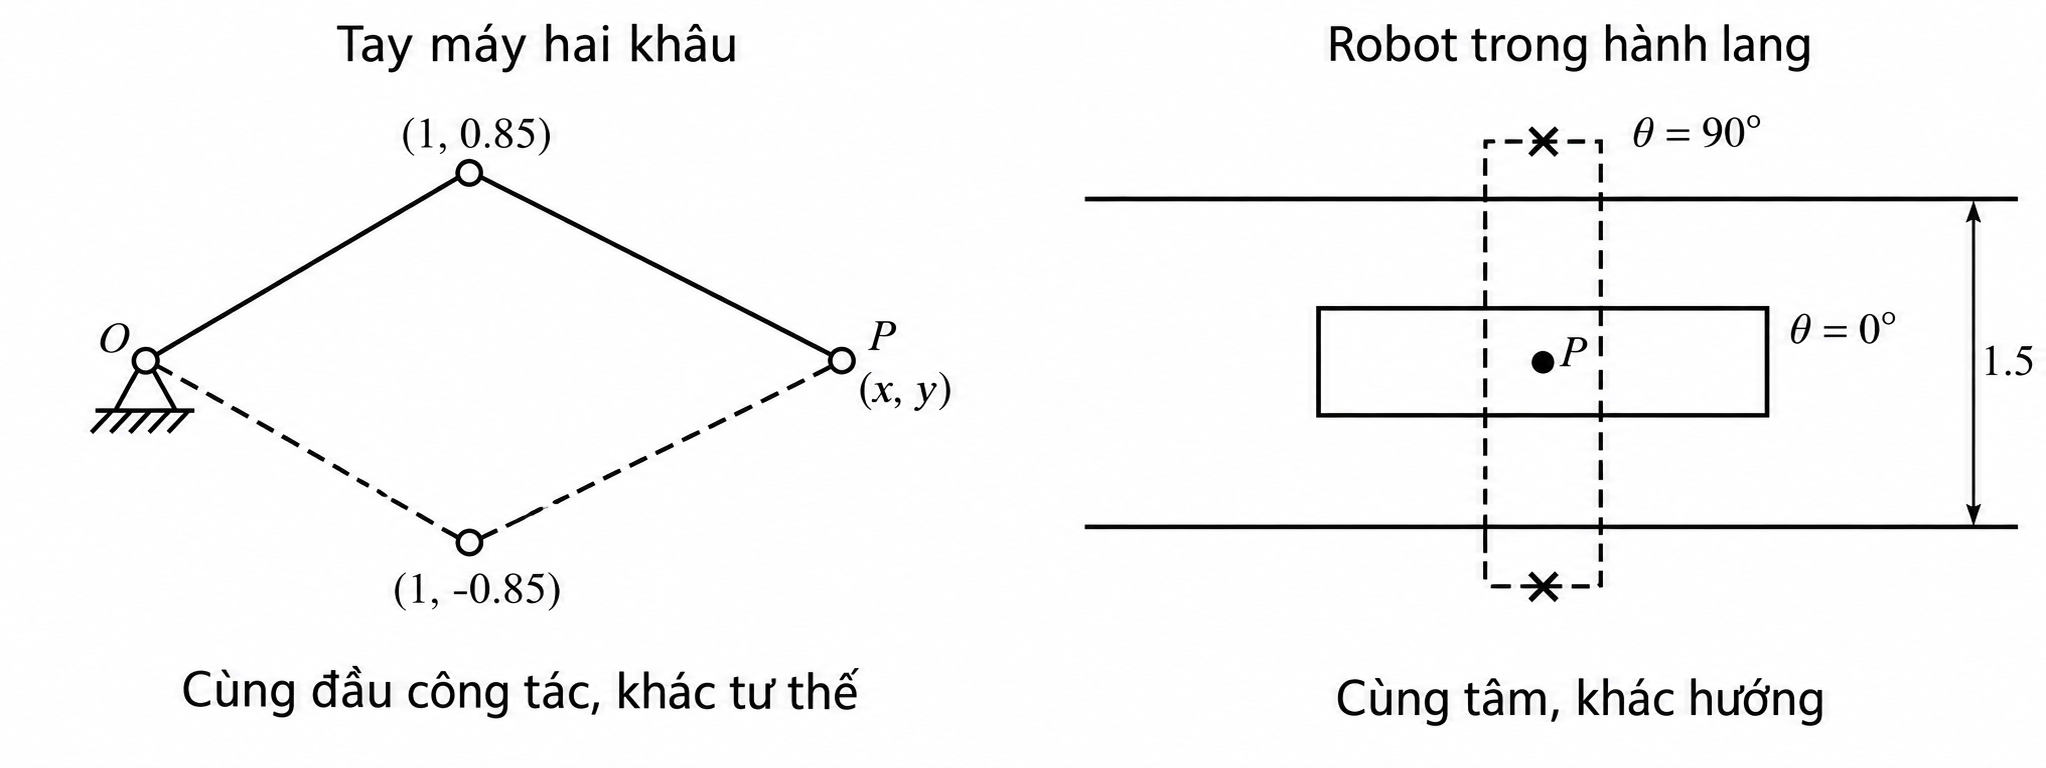
\includegraphics[width=\linewidth]{Same Position, Different Robot Configurations.png}
    \chuthichhinh[fig:workspace-configuration]{Cùng vị trí nhưng khác cấu hình robot}
  \end{center}
\end{minipage}\par\medskip

\subsection{\texorpdfstring{Biểu diễn vùng cấm \(C_{\mathrm{obs}}\) và kỹ thuật mở rộng vật cản hình học (Minkowski Sum).}{Biểu diễn vùng cấm C\_obs và kỹ thuật mở rộng vật cản hình học (Minkowski Sum).}}

\subsubsection*{a. Vùng cấm \(C_{\mathrm{obs}}\)}

Gọi \(A(q)\subset W\) là miền robot chiếm chỗ tại cấu hình \(q\), \(O=\bigcup_k O_k\) là hợp các vật cản. Vùng cấm trong không gian cấu hình được xác định bởi
\[
  C_{\mathrm{obs}}=\{q\in C\mid A(q)\cap O\neq\varnothing\},
  \qquad C_{\mathrm{free}}=C\setminus C_{\mathrm{obs}}.
\]
Theo quy ước này, tiếp xúc tại biên cũng được xem là va chạm. Khi biết bản đồ và hình học robot, một cấu hình được chấp nhận nếu toàn bộ thân robot nằm trong miền hoạt động cho phép và không giao với bất kỳ vật cản nào \cite{lavalle-planning-2006}.

Điều kiện không va chạm cho đường đi phải được áp dụng tại mọi điểm:
\[
  \gamma(0)=q_{\mathrm{start}},\quad
  \gamma(1)=q_{\mathrm{goal}},\quad
  \gamma(s)\in C_{\mathrm{free}},\quad \forall s\in[0,1].
\]
Kiểm tra riêng hai đầu một đoạn nối không bảo đảm phần giữa an toàn. Ví dụ, hai nút lưới có thể đều trống nhưng đoạn chéo nối chúng đi xuyên góc của một ô vật cản. Vì vậy, thuật toán cần kiểm tra cả cạnh nối, tránh cắt góc và kiểm tra lại các đoạn cong sau làm mượt.

Đường đi chỉ tồn tại về mặt hình học nếu điểm đầu và điểm đích thuộc cùng một thành phần liên thông theo đường của \(C_{\mathrm{free}}\). Khi một hành lang bị đóng kín sau mở rộng vật cản, việc tăng số vòng lặp tìm kiếm không tạo ra đường đi. Ngược lại, một hành lang quá hẹp so với độ phân giải có thể bị mất trên bản đồ rời rạc dù vẫn tồn tại trong mô hình liên tục; cần phân biệt bất khả thi hình học với hạn chế của biểu diễn.

\subsubsection*{b. Phân loại các loại va chạm}

\begin{center}
\begin{minipage}{\linewidth}
  \centering
  \refstepcounter{table}\label{tab:collision-types}%
  \tablename~\thetable: Phân loại các loại va chạm\par\smallskip
  \renewcommand{\arraystretch}{1.3}
  \begin{tabular}{@{}p{0.47\linewidth}p{0.47\linewidth}@{}}
    \toprule
    \textbf{Va chạm với môi trường} & \textbf{Tự va chạm} \\
    \midrule
    Một khâu hoặc thân robot giao với vật cản bên ngoài. & Hai bộ phận không được phép tiếp xúc của robot giao nhau. \\[4pt]
    \(A_i(q)\cap O\neq\varnothing\) & \(A_i(q)\cap A_j(q)\neq\varnothing\) \\
    \bottomrule
  \end{tabular}
\end{minipage}
\end{center}

Với robot gồm \(m\) bộ phận, miền cấm tổng hợp có thể viết
\[
  \begin{aligned}
    C_{\mathrm{obs}}={}&\bigcup_{i=1}^{m}
      \{q\in C\mid A_i(q)\cap O\neq\varnothing\}\\
    &\cup\bigcup_{(i,j)\in P}
      \{q\in C\mid A_i(q)\cap A_j(q)\neq\varnothing\},
  \end{aligned}
\]
trong đó \(P\) chỉ chứa những cặp cần kiểm tra. Các bộ phận lắp ghép có tiếp xúc được thiết kế sẵn phải được xử lý bằng mô hình phù hợp, tránh coi mọi tiếp xúc giữa hai khâu kề nhau là lỗi. Với xe ba bánh có khung cố định, kiểm tra thân xe với môi trường thường là trọng tâm; với tay máy, tự va chạm có thể loại bỏ nhiều cấu hình dù đầu công tác vẫn ở vị trí hợp lệ.

\noindent\textbf{Kỹ thuật mở rộng vật cản bằng tổng Minkowski.}

Cho hai tập hình học \(X,Y\subset\mathbb{R}^{2}\), tổng Minkowski được định nghĩa là
\[
  X\oplus Y=\{x+y\mid x\in X,\ y\in Y\}.
\]
Xét robot chỉ tịnh tiến với hướng cố định, gọi \(A_0\) là hình dạng robot trong hệ tọa độ có gốc tại điểm tham chiếu và \(p\) là vị trí gốc đó. Khi \(A(p)=p+A_0\), điều kiện va chạm tương đương với tồn tại \(a\in A_0,o\in O\) sao cho \(p+a=o\), hay \(p=o-a\). Suy ra vùng vị trí bị cấm là
\[
  C_{\mathrm{obs}}=O\oplus(-A_0),
  \qquad -A_0=\{-a\mid a\in A_0\}.
\]
Như vậy, thay vì dịch chuyển một vật thể có kích thước, có thể tìm đường cho điểm tham chiếu quanh vật cản đã mở rộng. Phép phản xạ \(-A_0\) cần được giữ trong công thức tổng quát; chỉ với hình đối xứng qua gốc mới có \(-A_0=A_0\) \cite{lavalle-planning-2006}.

Với robot được bao bởi đĩa bán kính \(r_b\), vật cản được nới ra theo mọi hướng một khoảng \(r_b\). Nếu vật cản tròn bán kính \(r_o\), vùng cấm của tâm xe là đĩa đồng tâm có bán kính \(r_o+r_b\). Với vật cản đa giác, vùng nới theo đĩa gồm các cạnh dịch ra ngoài và các cung tròn quanh đỉnh, không đơn thuần là tăng chiều rộng và chiều cao của một hình chữ nhật bao.

Nếu robot có thể xoay và có hình chữ nhật, vùng cấm phụ thuộc hướng:
\[
  C_{\mathrm{obs}}(\theta)=O\oplus[-R(\theta)A_0],
\]
trong đó \(R(\theta)\) là ma trận quay phẳng. Mỗi giá trị hướng tạo một lát cắt vật cản trong không gian \((x,y,\theta)\). Đĩa ngoại tiếp giúp tạo một bản đồ vị trí chung an toàn cho mọi hướng trong mô hình hình học, nhưng có thể loại bỏ các lối đi mà xe chỉ lọt khi xoay đúng hướng.

\noindent\textbf{Khoảng dự phòng và ví dụ tính toán.}

Để xét sai số kích thước, định vị và bám đường ở mức thiết kế, có thể chọn khoảng dự phòng \(\delta\geq0\), tạo
\[
  C_{\mathrm{obs}}^{\delta}
     =O\oplus(-A_0)\oplus B_{\delta},
\]
với \(B_{\delta}\) là đĩa bán kính \(\delta\). Biên bản đồ cũng phải được xử lý tương tự: tâm xe phải cách tường hoặc giới hạn vùng hoạt động đủ xa để cả thân xe nằm trong vùng cho phép. Khoảng dự phòng chỉ có ý nghĩa khi gắn với giả thiết về sai số; một giá trị chọn tùy ý chưa chứng minh được an toàn trong thực tế.

Ví dụ minh họa, giả sử xe được bao bởi đĩa \(r_b=0{,}15\,\mathrm{m}\), chọn \(\delta=0{,}05\,\mathrm{m}\). Hành lang giữa hai tường song song cần rộng hơn \(2(r_b+\delta)=0{,}40\,\mathrm{m}\) để tâm xe có một miền đi qua với độ rộng dương. Nếu hành lang rộng \(0{,}50\,\mathrm{m}\), dải khả dụng cho tâm xe còn \(0{,}10\,\mathrm{m}\). Đây là ví dụ tự xây dựng để giải thích phép mở rộng, không phải kích thước đã đo của mô hình đề tài.

Trên lưới có kích thước ô \(h\), cần nêu cách quy đổi khoảng mở rộng sang số ô và quy ước một ô được xem là bị chiếm. Làm tròn khoảng cách xuống hoặc chỉ kiểm tra tâm ô có thể bỏ sót va chạm ở biên. Sau khi tìm đường và làm mượt, phải kiểm tra đường mới trên cùng mô hình hình học; đường cong có thể tiến gần vật cản hơn các đoạn thẳng ban đầu.

\noindent\begin{minipage}{\linewidth}
  \begin{center}
    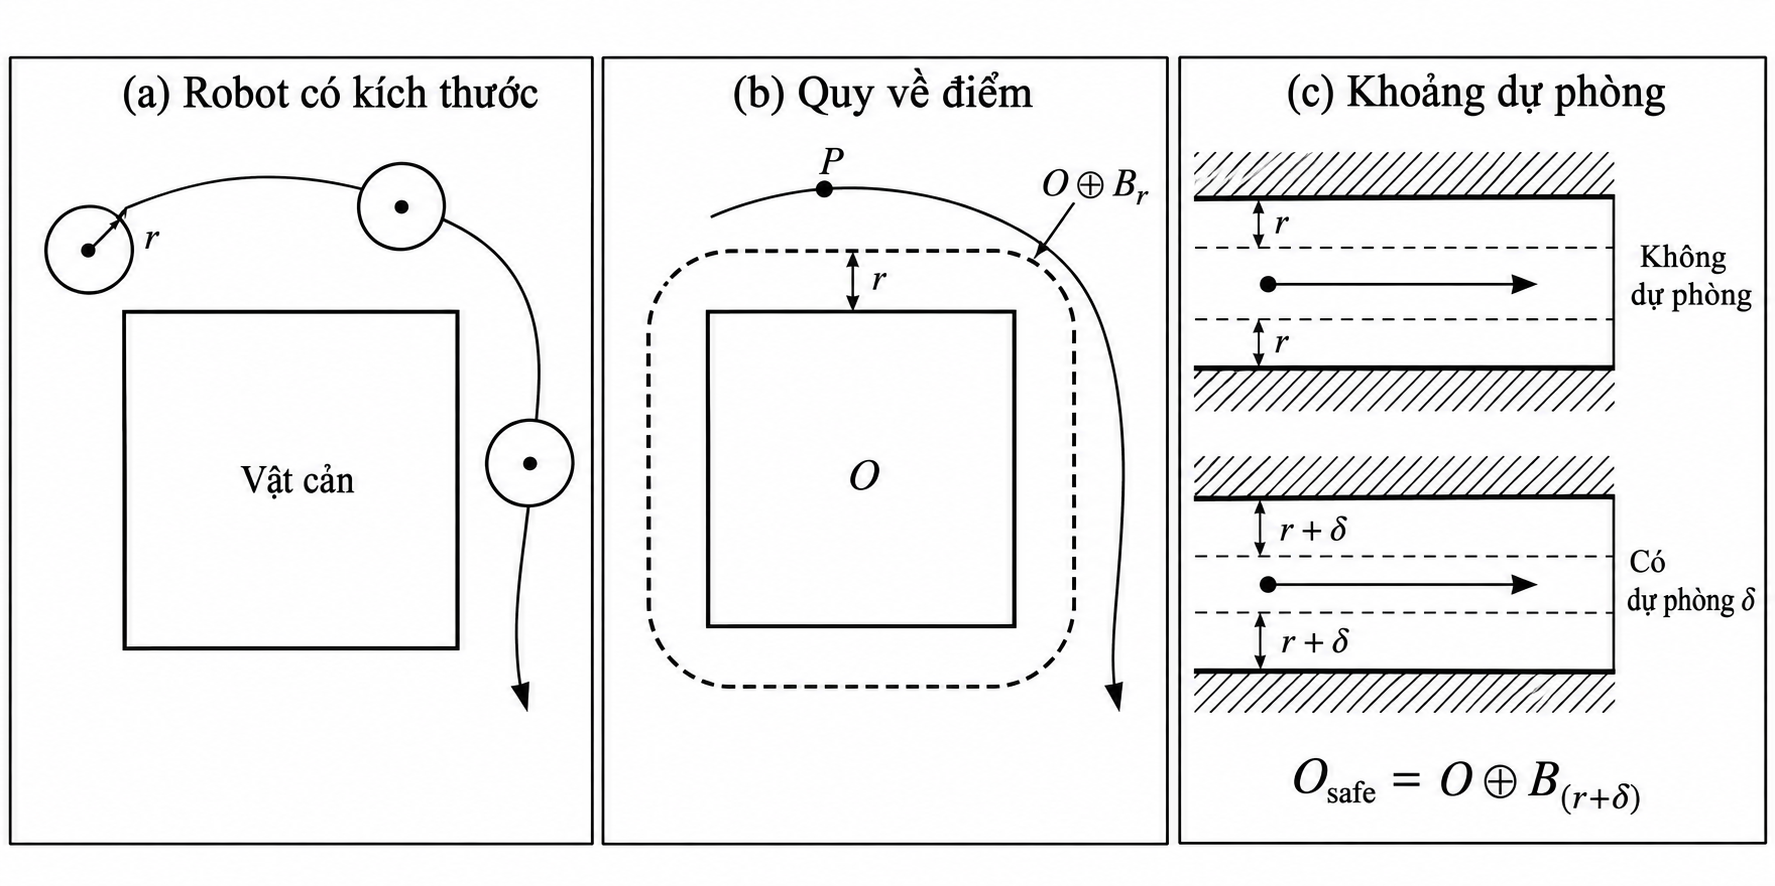
\includegraphics[width=\linewidth]{Minkowski expansion and robot safety clearance.png}
    \chuthichhinh[fig:minkowski-safety-clearance]{Mở rộng vật cản bằng tổng Minkowski và khoảng dự phòng}
  \end{center}
\end{minipage}\par\medskip

\section{Phân loại Toàn diện các Dạng Bài toán Quy hoạch Quỹ đạo}

Các dạng bài toán có thể được phân loại đồng thời theo yêu cầu chuyển động, cơ cấu, môi trường và hàm mục tiêu. Các tiêu chí này bổ sung cho nhau: một nhiệm vụ có thể vừa là chuyển động qua nhiều điểm, vừa dùng xe phi holonomic, vừa có vật cản động và ưu tiên giảm thời gian. Việc xác định đầy đủ các thuộc tính giúp chọn đúng mô hình thay vì gắn một thuật toán với mọi tình huống.

\subsection{Phân loại theo mục tiêu chuyển động: Điểm – Điểm (Point-to-Point - PTP) và Bám đường liên tục (Continuous Path - CP).}

\subsubsection*{a. Chuyển động điểm tới điểm (PTP)}

\textbf{Mô tả:} Robot di chuyển từ cấu hình ban đầu \(q_0\) tới cấu hình cuối \(q_f\), có thể kèm điều kiện vận tốc và gia tốc tại hai đầu. Hình dạng trung gian không được quy định trước, nhưng vẫn phải thỏa mãn giới hạn cơ cấu và tránh vật cản. Đối với xe vận chuyển, cấu hình đích có thể bao gồm cả hướng để xe ghép đúng với trạm nhận hàng.

Một mô hình biên thường gặp là
\[
  q(0)=q_0,\quad q(T)=q_f,\qquad
  \dot q(0)=\dot q(T)=0.
\]
Nếu robot đang chạy khi nhận mục tiêu mới, vận tốc đầu phải lấy theo trạng thái thực tại thời điểm chuyển tiếp. Đặt vận tốc tham chiếu về không tức thời có thể tạo lệnh giảm tốc không khả thi. Do đó, cập nhật mục tiêu phải đi kèm một đoạn nối thỏa mãn trạng thái hiện tại.

\textbf{Ứng dụng và tiêu chí đánh giá:} Gắp--đặt, hàn điểm, chuyển giữa các trạm và tiếp cận vị trí sạc. Chất lượng được đánh giá qua sai số đích, thời gian hoàn thành, khoảng cách tới vật cản và mức đáp ứng giới hạn vận tốc. Với tay máy nhiều khớp, cần đồng bộ thời gian kết thúc; cho từng khớp chạy nhanh nhất một cách độc lập có thể khiến chuyển động tổng thể thiếu phối hợp \cite{lynch-park-modern-robotics}.

\subsubsection*{b. Chuyển động bám theo đường đi liên tục (Continuous Path / Path Following Motion -- CP)}

\textbf{Mô tả:} Robot phải đi theo một đường hình học \(C(s)\) trong suốt quá trình thực hiện nhiệm vụ. Nếu thời điểm đi qua các điểm cũng được quy định, bài toán trở thành bám quỹ đạo có lịch thời gian. Nếu chỉ khống chế hình học, có thể điều chỉnh tốc độ dọc đường để đáp ứng giới hạn cơ cấu mà vẫn hoàn thành yêu cầu về đường đi.

Để làm rõ khác biệt, gọi \(p(t)\) là vị trí thực và \(p_d(t)=C(s_d(t))\) là vị trí mong muốn. Sai số bám quỹ đạo tại cùng thời điểm là \(\|p(t)-p_d(t)\|\), còn sai lệch hình học tới đường có thể định nghĩa bằng
\[
  e_{\mathrm{path}}(t)=\min_{s\in[0,1]}\|p(t)-C(s)\|.
\]
Robot có thể nằm đúng trên đường nhưng đi chậm hơn lịch, khi đó sai lệch hình học bằng không còn sai số bám quỹ đạo khác không. Khi đánh giá cần chọn chỉ tiêu phù hợp với yêu cầu nhiệm vụ.

\textbf{Ứng dụng và yêu cầu:} Hàn hồ quang, cắt, phun sơn và robot đi theo tuyến. Với tay máy, đường trong không gian thao tác phải được chuyển sang chuyển động khớp bằng động học ngược; cần bảo đảm nghiệm biến thiên liên tục và tránh kỳ dị. Với xe, phải liên hệ hướng thân xe với tiếp tuyến và kiểm tra độ cong, tốc độ quay cũng như giới hạn bánh xe. Bởi vậy, CP không đồng nghĩa với việc mọi loại robot đều giải cùng một bài toán động học ngược.

\subsubsection*{c. Chuyển động qua chuỗi điểm nút (Multipoint / Via-Points Trajectory)}

Quỹ đạo được mô tả qua chuỗi \(\{q_0,q_1,\ldots,q_N\}\), có hoặc không gắn thời điểm \(t_i\). Cần phân biệt yêu cầu đi qua chính xác từng nút với yêu cầu chỉ đi trong một vùng dung sai quanh nút. Điều kiện thứ hai cho phép bo góc để duy trì chuyển động liên tục; điều kiện thứ nhất có thể buộc robot giảm tốc hoặc dừng ở các nút đổi hướng đột ngột.

Nếu ghép hai đoạn tại \(t_i\), tính liên tục đến gia tốc được biểu diễn bởi
\[
  q(t_i^-)=q(t_i^+),\quad
  \dot q(t_i^-)=\dot q(t_i^+),\quad
  \ddot q(t_i^-)=\ddot q(t_i^+).
\]
Việc nội suy liên tục về vị trí chưa đủ bảo đảm chuyển động êm. Ngược lại, bo góc quá rộng có thể cắt vào vật cản hoặc bỏ qua vùng công nghệ bắt buộc. Trong đề tài, chuỗi nút từ thuật toán tìm đường được xem là đầu vào cho bước làm mượt; mỗi đường sau xử lý cần được kiểm tra lại về hình học và ràng buộc chuyển động.

\subsubsection*{d. Chuyển động bám đuổi đích động (Trajectory Tracking / Interception)}

Đích biến thiên theo thời gian, chẳng hạn vật trên băng chuyền hoặc robot dẫn đầu. Với bài toán đón bắt, thời điểm gặp \(T\) cũng có thể là biến cần tìm:
\[
  p_r(T)=p_{\mathrm{goal}}(T).
\]
Nếu yêu cầu tiếp xúc êm, còn cần ràng buộc vận tốc tương đối tại thời điểm gặp. Tìm đường tới vị trí đo gần nhất của mục tiêu có thể dẫn tới việc luôn đi sau mục tiêu; cần dự đoán chuyển động và cập nhật kế hoạch khi có quan sát mới.

Độ trễ cảm biến, thời gian tính toán và giới hạn gia tốc quyết định khả năng đón bắt. Khi dự đoán đích không đáng tin cậy, chỉ nên lập kế hoạch trong một khoảng dự báo phù hợp và tính lại theo trạng thái mới. Đây là yêu cầu khác với bám một quỹ đạo tham chiếu cố định: điều khiển bám thông thường không nhất thiết có một vật thể đích đang chuyển động trong môi trường.

\subsection{Phân loại theo đối tượng cơ cấu: Robot tay máy (Manipulator – Joint Space) và Robot di động (Mobile Robot – SE(2)/SE(3) Space).}

\subsubsection*{a. Tay máy công nghiệp (Serial \& Parallel Manipulators -- 6-DOF / 7-DOF)}

Tay máy được mô tả bằng tọa độ khớp \(q=(q_1,\ldots,q_n)\), trong đó có thể kết hợp khớp quay và khớp tịnh tiến. Một quỹ đạo cần thỏa mãn giới hạn vị trí, vận tốc, gia tốc khớp và tránh va chạm của toàn bộ các khâu. Với cơ cấu song song, các vòng động học còn tạo quan hệ liên kết giữa biến khớp; không thể xem mọi tọa độ là độc lập tùy ý.

Quan hệ vận tốc đầu công tác và vận tốc khớp có dạng \(V=J(q)\dot q\). Kỳ dị được nhận biết qua việc hạng của Jacobian giảm so với hạng cực đại của nó; biểu thức \(\det J=0\) chỉ phù hợp khi \(J\) vuông. Khi tiến gần kỳ dị, một vận tốc đầu công tác yêu cầu có thể dẫn tới vận tốc khớp rất lớn hoặc không thực hiện được. Với tay máy dư bậc tự do, có thể có nhiều chuyển động khớp tạo cùng chuyển động đầu công tác, từ đó xuất hiện khả năng chọn nghiệm để tránh vật cản hoặc giữ khoảng cách với giới hạn khớp \cite{lynch-park-modern-robotics}.

Tìm đường trong không gian khớp thuận tiện cho kiểm tra giới hạn khớp, nhưng không tự bảo đảm đầu công tác đi theo đường thẳng trong không gian thao tác. Ngược lại, một đường thẳng của đầu công tác có thể đi qua vùng không với tới hoặc bắt buộc đổi nhánh nghiệm. Sự lựa chọn không gian quy hoạch vì vậy cần xuất phát từ yêu cầu công nghệ cụ thể.

\subsubsection*{b. Robot di động bánh xe (AGV / AMR)}

Robot bánh xe được phân biệt theo khả năng tạo vận tốc tức thời. Cơ cấu đa hướng được bố trí phù hợp có thể tạo chuyển động phẳng theo ba thành phần vận tốc thân xe; xe vi sai và xe lái kiểu ô tô chịu ràng buộc không trượt ngang. Với mô hình vi sai lý tưởng,
\[
  \dot x=v\cos\theta,\qquad
  \dot y=v\sin\theta,\qquad \dot\theta=\omega,
\]
suy ra \(\dot x\sin\theta-\dot y\cos\theta=0\). Xe có ba biến tư thế nhưng chỉ có hai ngõ vào vận tốc độc lập \(v,\omega\). Điều này không làm mất khả năng tới các vị trí trên mặt phẳng bằng một chuỗi thao tác; nó hạn chế hướng chuyển động tức thời \cite{lynch-park-modern-robotics}.

\textbf{Phân biệt giới hạn quay vòng:} Xe Ackermann với chiều dài cơ sở \(L_a\) và góc lái cực đại \(\delta_{\max}\) có bán kính quay tối thiểu theo mô hình xe đạp
\[
  R_{\min}=\frac{L_a}{\tan\delta_{\max}}.
\]
Trong khi đó, xe vi sai lý tưởng có thể quay tại chỗ khi hai bánh quay ngược chiều, nên không có cùng giới hạn bán kính dương do góc lái. Khả năng quay thực tế còn phụ thuộc vùng quét thân xe, bánh tự lựa, ma sát và giới hạn truyền động. Không nên áp dụng trực tiếp mô hình xe ô tô cho mọi robot phi holonomic.

Đường Dubins phù hợp với mô hình xe chỉ tiến và bị chặn độ cong; Reeds--Shepp cho phép thêm chuyển động lùi. Clothoid có độ cong biến thiên tuyến tính theo chiều dài cung, còn Bézier và B-Spline là công cụ biểu diễn đường cong. Các đường này chỉ phù hợp khi điều kiện mô hình và ràng buộc cơ cấu được kiểm tra, chứ không phải cứ chọn một đường trơn là xe bám được \cite{lavalle-planning-2006}.

Đối với robot ba bánh của đề tài, hai bánh chủ động quyết định chuyển động, bánh tự lựa đỡ khung xe. Bộ quy hoạch cần tạo \(v(t),\omega(t)\), sau đó quy đổi thành vận tốc bánh trái và phải theo bán kính bánh và khoảng cách hai bánh. Kiểm tra giới hạn ở từng bánh giúp phát hiện trường hợp vận tốc tâm xe còn nhỏ nhưng bánh phía ngoài cua đã vượt khả năng truyền động.

\subsubsection*{c. Robot bay (Unmanned Aerial Vehicles -- UAV / Quadrotors)}

Quadrotor có sáu bậc tự do tư thế nhưng trong mô hình thông dụng chỉ tạo được lực đẩy tổng và ba mô-men điều khiển độc lập. Chuyển động ngang đòi hỏi nghiêng thân để đổi hướng lực đẩy, nên vị trí và hướng nghiêng liên hệ qua động lực học. Đây là ví dụ cho thấy một đường trong không gian 3D chưa đủ xác định một chuyển động khả thi.

Tính phẳng vi phân cho phép khai thác các biến đầu ra \((x,y,z,\psi)\) và các đạo hàm của chúng để tái dựng trạng thái, ngõ vào trong miền mô hình phù hợp. Một hướng tạo chuyển động êm là tối ưu bình phương đạo hàm bậc bốn của vị trí theo thời gian (minimum snap). Tuy nhiên, quỹ đạo còn phải đáp ứng giới hạn lực đẩy, góc nghiêng và tốc độ quay; tránh vật cản cũng cần xét kích thước và tư thế thân máy bay \cite{bry-flatness-flight}.

So với xe trong đề tài, robot bay đòi hỏi mô hình động lực học và đánh giá khả thi phức tạp hơn. Nhóm này được đưa vào hệ thống phân loại nhằm làm rõ tính đa dạng của bài toán, không thuộc phần cài đặt và thực nghiệm của đề tài.

\subsubsection*{d. Robot chân bước \& robot hình người (Legged \& Humanoid Robots)}

Quy hoạch cho robot chân bước phải xác định cả chuyển động thân và chuỗi tiếp xúc: chân nào chống, chân nào vung và thời điểm đổi pha. Mỗi pha có tập ràng buộc khác nhau, tạo thành hệ động lực học lai. Một bước chân tránh được vật cản vẫn có thể không khả thi nếu lực tiếp xúc yêu cầu vượt giới hạn ma sát hoặc làm mất cân bằng.

Trong mô hình đơn giản với các tiếp xúc đồng phẳng, có thể dùng điều kiện ZMP nằm trong miền hỗ trợ để hỗ trợ kiểm tra cân bằng động; tính khả thi tiếp xúc còn liên quan tới lực ma sát và mô-men tại bàn chân \cite{caron-contact-stability-2015}. Với cân bằng tĩnh trên mặt phẳng ngang, hình chiếu khối tâm phải nằm trong miền hỗ trợ. Không thể đồng nhất điều kiện tĩnh này với một điều kiện đầy đủ cho mọi chuyển động động lực học.

Như vậy, cùng một nhiệm vụ vượt vật cản có thể dẫn tới các biến quyết định khác nhau: xe cần một chuyển động lăn khả thi, tay máy cần phối hợp khớp, robot chân bước cần thêm chuỗi tiếp xúc. Sự khác biệt này giải thích vì sao đề tài giới hạn triển khai vào xe vi sai thay vì dùng một mô hình chung cho tất cả cơ cấu.

\subsection{Phân loại theo môi trường hoạt động: Môi trường tĩnh, môi trường động và môi trường không xác định.}

Mức độ biến đổi của môi trường và mức độ hiểu biết về môi trường là hai thuộc tính độc lập. Một phòng có vật cản đứng yên vẫn có thể là môi trường chưa biết nếu robot chưa có bản đồ. Ngược lại, vật cản chuyển động có thể có quy luật đã biết trước. Việc tách hai thuộc tính giúp xác định nhu cầu cảm biến, dự đoán và cập nhật kế hoạch.

\subsubsection*{a. Môi trường tĩnh và biết trước hoàn toàn (Known Static Environment)}

Bản đồ, hình học vật cản và giới hạn miền hoạt động được xem là đã biết, không thay đổi trong thời gian nhiệm vụ. Với robot có hình dạng cố định, \(C_{\mathrm{obs}}\) không phụ thuộc thời gian. Đây là điều kiện phù hợp để xây dựng và so sánh các thuật toán tìm đường cơ sở trên cùng một bộ bản đồ.

Dijkstra và A* tìm đường trên đồ thị hoặc lưới đã xây dựng; PRM có thể tái sử dụng một mạng đường cho nhiều truy vấn; RRT và RRT* phát triển cấu trúc lấy mẫu để nối điểm đầu với đích. Tính tối ưu của đường cần được hiểu theo mô hình tương ứng: tối ưu trên đồ thị rời rạc không đồng nghĩa tối ưu trong không gian liên tục, còn tối ưu tiệm cận không bảo đảm nghiệm tốt nhất sau một số mẫu hữu hạn.

Môi trường tĩnh vẫn có thể đòi hỏi giới hạn thời gian tính toán khi robot nhận nhiệm vụ liên tiếp. Vì vậy, đánh giá cần ghi cả thời gian tiền xử lý và thời gian truy vấn. Nếu một phương pháp được phép xây mạng trước còn phương pháp khác bị tính toàn bộ thời gian khởi tạo vào truy vấn, kết quả so sánh phải công bố rõ cách tính đó.

\subsubsection*{b. Môi trường động (Dynamic Environment)}

Vật cản thay đổi vị trí theo thời gian nên vùng cấm trở thành \(C_{\mathrm{obs}}(t)\). Điều kiện tránh va chạm của quỹ đạo là
\[
  q(t)\notin C_{\mathrm{obs}}(t),\qquad t\in[0,T].
\]
Hai chuyển động đi qua cùng một điểm hình học có thể an toàn nếu đến vào các thời điểm khác nhau. Ngược lại, một đường không giao với vị trí hiện tại của vật cản vẫn có thể va chạm ở tương lai. Thời gian vì vậy phải tham gia vào việc đánh giá thay vì chỉ được gán sau khi chốt đường đi \cite{lavalle-planning-2006}.

Ví dụ, xe và người cùng tiếp cận một cửa hẹp có thể tránh xung đột bằng cách xe giảm tốc và chờ, dù tuyến hình học không đổi. Một phương án vòng tránh dài hơn chỉ tốt hơn nếu phù hợp với khả năng dự đoán, khoảng trống và giới hạn điều khiển. Đây là cơ sở để kết hợp tuyến toàn cục với bộ xử lý cục bộ tính lại chuyển động trong một khoảng thời gian gần.

DWA, TEB và MPC là những hướng thường được khảo sát ở tầng cục bộ, nhưng tên thuật toán không tự bảo đảm tránh được mọi vật cản động. Khả năng xử lý phụ thuộc mô hình dự đoán, dữ liệu đầu vào, giới hạn vận tốc và thời gian cập nhật. Trong đề tài, tình huống động chỉ được xét ở mức mô phỏng cơ bản; việc thực nghiệm đòi hỏi cảm biến và cơ chế dừng phù hợp.

\subsubsection*{c. Môi trường chưa biết trước hoặc nhận thức bán phần (Unknown / Partially Known)}

Robot chỉ quan sát được một vùng hữu hạn và phải cập nhật bản đồ từ cảm biến. Ô chưa quan sát cần được phân biệt với ô tự do. Nếu coi toàn bộ vùng chưa biết là trống, thuật toán có thể tạo một tuyến chưa được xác nhận an toàn; nếu coi tất cả là vật cản, robot có thể không tìm được đường để tiến hành khám phá.

Cần quy định chính sách xử lý vùng chưa biết, vùng quan sát tối thiểu trước xe và thời điểm tính lại kế hoạch. Khi phát hiện vật cản mới, hệ thống có thể cập nhật tuyến toàn cục, điều chỉnh đoạn chuyển động gần hoặc dừng chờ. Nếu bản đồ chưa được xây dựng và vị trí robot cũng chưa biết, có thể cần SLAM; nếu đã có bản đồ phù hợp thì bài toán có thể chỉ cần định vị trên bản đồ đó.

Độ trễ quyết định khoảng dự phòng theo hướng chuyển động. Với vật cản đứng yên và giả thiết giảm tốc không đổi \(a_b>0\), một ước lượng thiết kế là
\[
  d_{\mathrm{req}}=v\tau+\frac{v^2}{2a_b}+d_m,
\]
trong đó \(\tau\) là độ trễ tổng và \(d_m\) là khoảng dự phòng. Biểu thức được suy ra từ quãng đường đi trong độ trễ và quãng đường phanh, không phải bảo đảm cho mọi tình huống. Vật cản đang tiến tới, sàn trơn hoặc sai số định vị cần được xem xét thêm. Quan hệ này cũng cho thấy không thể chọn tốc độ chỉ từ công suất động cơ mà bỏ qua tầm quan sát.

\subsubsection*{d. Môi trường không gian hẹp và phức tạp (Cluttered Environment \& Narrow Passages)}

Không gian hẹp là đặc điểm hình học có thể xuất hiện trong cả môi trường tĩnh lẫn động. Khó khăn thường nằm ở một đoạn nối hẹp giữa hai vùng trống lớn; tổng diện tích tự do vẫn có thể lớn. Vì vậy, tỉ lệ diện tích tự do toàn bản đồ không đủ mô tả độ khó của bài toán.

Với lấy mẫu đều, xác suất rơi vào một hành lang nhỏ có thể thấp, khiến hai vùng đã khám phá chưa nối được với nhau. Với lưới, hành lang có thể biến mất nếu ô quá lớn; tăng độ phân giải lại làm số nút tăng nhanh. Các hướng như Gaussian sampling hoặc bridge sampling tập trung mẫu gần cấu trúc vật cản, nhưng vẫn cần kiểm tra đường nối và giới hạn cơ cấu.

Đối với xe chữ nhật, cần tính cả vùng quét khi đổi hướng tại cửa hoặc góc cua. Một đoạn thẳng đủ rộng chưa chứng minh xe quay được ở cuối đoạn. Việc làm mượt sau tìm đường cũng cần bị giới hạn trong hành lang an toàn, tránh làm tròn góc theo cách đưa thân xe vào vật cản.

Các kịch bản so sánh trong đề tài cần thay đổi có kiểm soát bề rộng hành lang, số góc rẽ và khoảng dự phòng. Khi một phương pháp thất bại, phải ghi rõ hết thời gian, hết số mẫu, không nối được cạnh hay không tồn tại đường khả thi trong mô hình, thay vì chỉ báo chung là không tìm thấy đường.

\subsection{Phân loại theo hàm mục tiêu tối ưu: Tối ưu thời gian (Time-optimal), Tối ưu năng lượng (Energy-optimal), Tối ưu độ giật (Minimum Jerk).}

Hàm mục tiêu mô tả tiêu chí lựa chọn giữa các quỹ đạo khả thi. Một bài toán tổng quát có thể viết
\[
  \min_{T,z(\cdot),u(\cdot)} J
  =\Phi(z(T),T)+\int_0^T \mathcal{L}(z(t),u(t))\,dt,
\]
với ràng buộc mô hình \(\dot z=f(z,u)\), điều kiện đầu cuối, tránh va chạm và giới hạn chấp hành. Trong đó, \(z\) là trạng thái còn \(u\) là ngõ vào điều khiển. Cần tách các ràng buộc bắt buộc khỏi tiêu chí ưu tiên: một nghiệm có giá trị mục tiêu thấp nhưng va chạm hoặc vượt khả năng động cơ không được chấp nhận.

\noindent\textbf{Tối ưu thời gian.}

Mục tiêu là giảm thời gian chuyển động \(J_T=T\). Cần phân biệt thời gian robot thực hiện nhiệm vụ với thời gian máy tính tìm ra quỹ đạo. Thuật toán trả lời nhanh có thể tạo đường dài, buộc xe chạy chậm ở nhiều góc; ngược lại, quỹ đạo thực hiện nhanh có thể cần nhiều thời gian tối ưu trước khi xuất phát.

Khi hình học đường đi đã cố định, bài toán có thể chuyển thành tìm quy luật thời gian \(s(t)\). Với \(q=q(s)\), ta có
\[
  \dot q=q_s\dot s,\qquad
  \ddot q=q_s\ddot s+q_{ss}\dot s^2,
\]
trong đó \(q_s=dq/ds\). Giới hạn vận tốc, gia tốc hoặc mô-men tạo ra miền cho phép của \(\dot s,\ddot s\); thời gian ngắn nhất phải được tìm trong miền này \cite{lynch-park-modern-robotics}. Trong mô hình đơn giản chỉ giới hạn vận tốc và gia tốc, nghiệm có thể gồm các pha tăng tốc, chạy đều và giảm tốc. Khi thêm giới hạn jerk, các chỗ đổi gia tốc phải có giai đoạn chuyển tiếp.

Đối với xe, giới hạn tốc độ qua cua còn gắn với gia tốc pháp tuyến \(a_n=v^2|\kappa|\). Nếu chọn ngưỡng thiết kế \(a_{n,\max}\), điều kiện sơ bộ tại điểm có \(\kappa\neq0\) là \(v\leq\sqrt{a_{n,\max}/|\kappa|}\). Như vậy, một tuyến ngắn nhiều góc gắt có thể mất thời gian hơn một tuyến dài nhưng cong thoải. Giá trị ngưỡng phải được xác định phù hợp với xe và điều kiện thử.

\noindent\textbf{Tối ưu năng lượng.}

Năng lượng điện lấy từ nguồn có thể mô tả bởi \(E=\int_0^T P_{\mathrm{source}}(t)\,dt\), với quy ước công suất và khả năng thu hồi năng lượng được nêu rõ. Trong mô phỏng truyền động đơn giản, có thể xem xét các thành phần tổn hao như \(\int i^2R\,dt\). Tuy nhiên, tích phân bình phương vận tốc, gia tốc hoặc tín hiệu điều khiển chỉ là chỉ tiêu thay thế, chưa tương đương với điện năng tiêu thụ.

Tăng thời gian chuyển động có thể làm giảm yêu cầu tăng tốc nhưng lại kéo dài thời gian cấp nguồn cho mạch điều khiển và cảm biến. Mặt khác, tải, ma sát, hiệu suất hộp số và tổn hao driver có thể thay đổi theo chế độ vận hành. Vì vậy, không thể suy ra rằng đường ngắn nhất hoặc chuyển động chậm nhất luôn tiết kiệm năng lượng nhất.

Trong phạm vi đề tài chủ yếu dùng động học, năng lượng được trình bày như một hướng phân loại và mở rộng. Nếu chưa có mô hình dòng điện hoặc phép đo công suất thì chỉ báo cáo các đại lượng đã tính được, chẳng hạn quãng đường và số lần tăng giảm tốc; không gọi chúng là kết quả đo tiết kiệm năng lượng.

\noindent\textbf{Tối ưu độ giật.}

Độ giật là đạo hàm theo thời gian của gia tốc: \(j(t)=\dddot q(t)\). Một chỉ tiêu phổ biến để mô tả mức biến thiên nhanh của gia tốc là
\[
  J_j=\int_0^T \|\dddot q(t)\|^2\,dt.
\]
Khi các tọa độ có đơn vị khác nhau, cần chuẩn hóa hoặc dùng ma trận trọng số thay cho cộng trực tiếp các thành phần. Giảm \(J_j\) và áp dụng ràng buộc cứng \(|j_i(t)|\leq j_{i,\max}\) cũng là hai yêu cầu khác nhau: tích phân nhỏ không tự loại trừ một đỉnh jerk lớn trong khoảng thời gian ngắn.

Ảnh hưởng của thời gian có thể được thấy bằng phép đổi biến \(\tau=t/T\). Nếu giữ nguyên hình dạng chuẩn hóa \(q(t)=\bar q(\tau)\), thì \(\dddot q=T^{-3}\bar q^{(3)}\), do đó
\[
  J_j=T^{-5}\int_0^1\|\bar q^{(3)}(\tau)\|^2\,d\tau.
\]
Đây là hệ quả trực tiếp của quy tắc đạo hàm. Nếu chỉ giảm jerk mà không chặn thời gian, có thể làm chỉ tiêu nhỏ đi bằng cách cho robot chạy rất chậm. Do đó, so sánh độ êm cần cố định thời gian hoặc công bố rõ cách đánh đổi giữa jerk và thời gian hoàn thành.

\noindent\textbf{Đánh đổi nhiều mục tiêu và tiêu chí áp dụng.}

Một dạng kết hợp có thể dùng là
\[
  J=w_T\frac{T}{T_{\mathrm{ref}}}
    +w_L\frac{L_p}{L_{\mathrm{ref}}}
    +w_j\frac{J_j}{J_{j,\mathrm{ref}}},
  \qquad w_T,w_L,w_j\geq0,
\]
trong đó \(L_p\) là chiều dài đường đi và các mẫu số dương dùng để chuẩn hóa đơn vị. Trọng số biểu thị ưu tiên và cần được công bố; thay đổi thang đo mà không chuẩn hóa có thể làm thay đổi nghiệm dù ý định ưu tiên không đổi.

Trong đề tài, tránh va chạm và đáp ứng giới hạn chuyển động được đặt thành điều kiện chấp nhận trước khi so sánh chiều dài, thời gian tính toán và độ trơn. Các chỉ tiêu được báo cáo riêng để thấy rõ đánh đổi. Khi chưa xác định ưu tiên của một ứng dụng cụ thể, kết luận nên chỉ ra phương án phù hợp với từng tiêu chí thay vì khẳng định có một thuật toán tốt nhất trong mọi môi trường.

\noindent\begin{minipage}{\linewidth}
  \begin{center}
    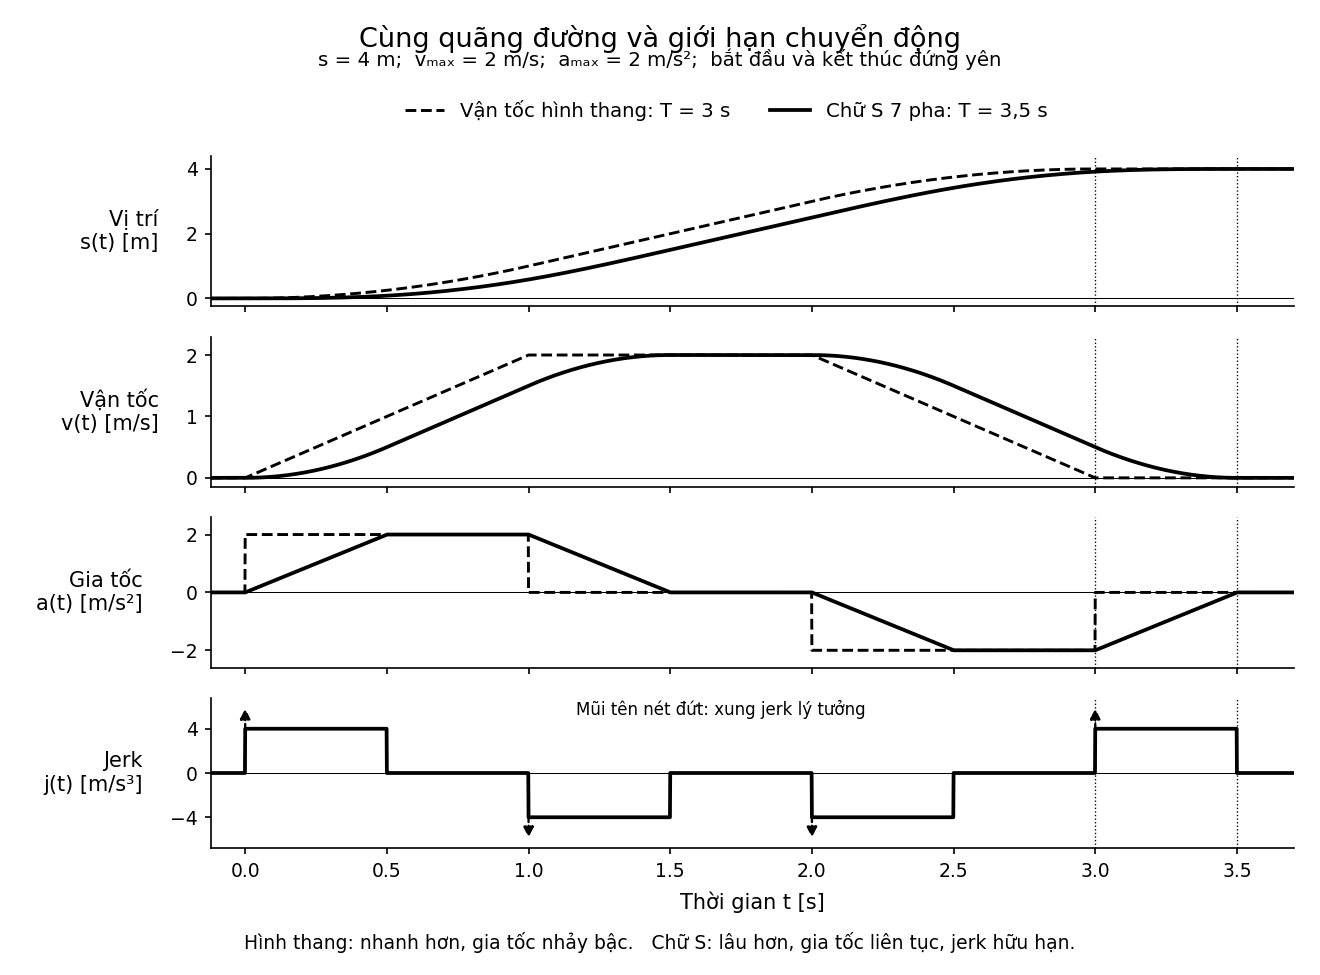
\includegraphics[width=\linewidth]{so_sanh_quy_luat_chuyen_dong_v2.png}
    \chuthichhinh[fig:motion-profile-comparison]{So sánh các quy luật chuyển động và độ êm quỹ đạo}
  \end{center}
\end{minipage}\par\medskip

\section{Đối tượng Nghiên cứu, Mục tiêu và Giới hạn Phạm vi Đề tài}

\subsection{Đối tượng nghiên cứu}

Đối tượng nghiên cứu gồm các dạng bài toán quy hoạch chuyển động và chuỗi xử lý chuyển từ yêu cầu nhiệm vụ sang quỹ đạo tham chiếu khả thi cho robot. Nội dung được tổ chức theo ba lớp liên hệ: mô hình hình học để tìm đường tránh vật cản, mô hình động học để kiểm tra khả năng thực hiện và quy luật thời gian để xác định vị trí, vận tốc, gia tốc theo thời gian.

\textbf{Hệ thống robot mục tiêu:} Xe di động ba bánh, gồm hai bánh chủ động độc lập và một bánh tự lựa, chuyển động trên mặt phẳng. Tư thế thân xe được biểu diễn bằng \(q=(x,y,\theta)\); ở mức động học, ngõ vào là vận tốc tịnh tiến \(v\) và vận tốc quay \(\omega\). Kích thước thân, bán kính bánh và khoảng cách hai bánh là các tham số cần đưa vào kiểm tra khả thi, thay vì chỉ mô hình hóa robot như điểm không có kích thước.

\textbf{Đầu vào và đầu ra của bài toán:} Đầu vào gồm bản đồ, hình học robot, trạng thái đầu, yêu cầu đích và các giới hạn chuyển động. Đầu ra tìm đường là một chuỗi nút hoặc đường hình học; đầu ra tạo quỹ đạo là chuỗi tham chiếu có dấu thời gian. Một giao diện mong muốn có dạng
\[
  \mathcal{T}_{\mathrm{ref}}=
    \{t_k,x_k,y_k,\theta_k,v_k,\omega_k\}_{k=0}^{N}.
\]
Chuỗi này phải sử dụng cùng hệ tọa độ và đơn vị với bộ điều khiển. Chất lượng tìm đường, chất lượng gán thời gian và sai số bám được đánh giá riêng để xác định đúng nguồn sai lệch.

\textbf{Các phương pháp khảo sát:} Nhóm đồ thị gồm Dijkstra, A*; nhóm lấy mẫu gồm PRM, RRT, RRT*; nhóm trường lực gồm APF và phương án khắc phục cực tiểu cục bộ. Phần tạo chuyển động xem xét nội suy đa thức, profile vận tốc hình thang, profile chữ S và làm mượt bằng đường cong tham số. Các phương pháp không nhất thiết giải cùng một bài toán ở cùng cấp; cần xác định rõ vai trò trước khi so sánh.

\subsection{Mục tiêu nghiên cứu}

\subsubsection*{a. Mục tiêu tổng quát}

Hệ thống hóa các dạng bài toán quy hoạch quỹ đạo trong điều khiển robot, xây dựng quy trình tìm đường--làm mượt--gán thời gian cho xe vi sai, từ đó đánh giá khả năng tạo chuyển động an toàn và khả thi trong mô phỏng, đồng thời xây dựng phương án kiểm chứng trên mô hình robot ba bánh.

Kết quả cần làm rõ mối liên hệ giữa thuật toán và điều kiện áp dụng: loại môi trường nào phù hợp, ràng buộc nào đã được xét và tiêu chí nào được cải thiện. Tính hiệu quả phải dựa trên các kịch bản và dữ liệu kiểm chứng; phần triển khai phần cứng được dùng để đánh giá khoảng cách giữa quỹ đạo tham chiếu và chuyển động thực tế.

\subsubsection*{b. Mục tiêu cụ thể}

\begin{itemize}
  \item \textbf{Hệ thống hóa khái niệm và mô hình bài toán:} Phân biệt đường đi, quỹ đạo và điều khiển bám; xây dựng biểu diễn cấu hình, vùng cấm và khoảng dự phòng. Sản phẩm cần có là các định nghĩa nhất quán, điều kiện đầu cuối và mô hình kiểm tra va chạm dùng chung cho các thuật toán.
  \item \textbf{Phân tích ràng buộc của robot vi sai:} Thiết lập quan hệ giữa vận tốc thân xe và vận tốc bánh, làm rõ ràng buộc không trượt ngang và khả năng quay tại chỗ. Qua đó xác định vì sao một đường hình học hợp lệ có thể cần làm mượt hoặc giảm tốc mới thực hiện được.
  \item \textbf{Xây dựng các profile chuyển động:} Khảo sát đa thức bậc ba, bậc năm, vận tốc hình thang và chữ S; đối chiếu điều kiện biên, mức liên tục và giới hạn vận tốc, gia tốc, jerk. Các ví dụ sử dụng cùng điều kiện dịch chuyển khi mục đích là so sánh tính chất profile.
  \item \textbf{Cài đặt và phân tích các nhóm thuật toán tìm đường:} Mô tả đầu vào, đầu ra, quy tắc mở rộng và điều kiện dừng của Dijkstra, A*, PRM, RRT, RRT* và APF. Làm rõ những trường hợp thất bại và ý nghĩa của các bảo đảm lý thuyết khi triển khai với tài nguyên hữu hạn.
  \item \textbf{Kết nối tìm đường với tạo quỹ đạo:} Chuyển chuỗi nút thành đường cong phù hợp, kiểm tra lại va chạm và gán quy luật thời gian. Đầu ra cần đủ thông tin cho điều khiển bám, không dừng ở một hình vẽ đường đi trên bản đồ.
  \item \textbf{Thiết lập quy trình so sánh định lượng:} Dùng các kịch bản chung, cùng hình học robot và cùng quy tắc chấp nhận nghiệm; báo cáo chiều dài, thời gian tính toán, tỉ lệ thành công, khoảng cách an toàn và độ trơn sau xử lý. Với phương pháp ngẫu nhiên, cần nhiều lần chạy và ghi tham số để đánh giá độ biến thiên.
  \item \textbf{Đề xuất và kiểm chứng triển khai thực nghiệm:} Xây dựng giao diện tham chiếu, ước lượng chuyển động từ encoder và điều khiển tốc độ bánh trên mô hình ba bánh theo nội dung Chương IV. Việc kết luận về độ chính xác bám, độ lặp lại hoặc tránh vật cản thực tế chỉ thực hiện khi có nhật ký và phép đo đối chứng phù hợp.
\end{itemize}

Để các mục tiêu có thể kiểm tra, mỗi kết quả cần gắn với một minh chứng: phương trình và điều kiện áp dụng cho phần lý thuyết; mã và cấu hình cho phần thuật toán; bảng chỉ tiêu cùng bản đồ cho mô phỏng; dữ liệu đo cho thực nghiệm. Khi chưa có dữ liệu, nội dung được trình bày dưới dạng phương án và tiêu chí đánh giá, không thay bằng kết quả giả định.

\subsection{Giới hạn phạm vi đề tài}

\subsubsection*{a. Phạm vi về không gian và môi trường}

\textbf{Không gian hoạt động:} Đề tài tập trung vào mặt phẳng 2D với robot có kích thước hữu hạn. Mô hình cơ sở giả thiết mặt sàn tương đối phẳng, bánh tiếp xúc liên tục và vận hành trong miền tốc độ phù hợp với giả thiết lăn không trượt. Địa hình dốc, chướng ngại có thể vượt qua bằng nâng bánh và chuyển động 3D không nằm trong phần triển khai chính.

\textbf{Bản đồ và vật cản:} Mô phỏng chính sử dụng bản đồ biết trước, biểu diễn bằng ô lưới hoặc các miền hình học phẳng, với vật cản tĩnh. Điểm đầu và đích phải hợp lệ sau khi xét kích thước robot và khoảng dự phòng. Các kịch bản gồm không vật cản, mê cung, mật độ vật cản cao và hành lang hẹp để khảo sát những đặc điểm khó khác nhau.

\textbf{Tình huống động và chưa biết:} Chỉ xem xét một số tình huống mô phỏng có quy luật chuyển động hoặc cập nhật vật cản được chỉ rõ. Chưa đặt mục tiêu giải quyết tổng quát dự đoán hành vi con người, phối hợp nhiều robot hoặc tự xây dựng bản đồ trong mọi môi trường. Các hướng SLAM và quy hoạch động thời gian thực được trình bày ở mức mở rộng, phù hợp với năng lực cảm biến được bổ sung sau này.

Trong thử nghiệm phòng thí nghiệm, kết luận bị giới hạn bởi kích thước khu vực, cách bố trí vật cản và điều kiện quan sát đã ghi nhận. Một mô hình chạy được trên bản đồ đã biết chưa chứng minh khả năng tự hành an toàn trong nhà kho có người và xe nâng hoạt động.

\subsubsection*{b. Giới hạn về mặt kỹ thuật và mô hình hóa}

\textbf{Mô hình và truyền động:} Phần quy hoạch dùng chủ yếu mô hình động học vi sai. Giới hạn vận tốc và gia tốc được đưa vào ở mức thiết kế quỹ đạo; chưa xây dựng đầy đủ động lực học tiếp xúc, độ đàn hồi truyền động, tải biến thiên và mô hình điện--cơ đã nhận dạng. Các nhận xét về năng lượng, trượt và rung cần được phân biệt với kết quả đo trực tiếp.

\textbf{Mức triển khai điều khiển:} Trọng tâm là quy hoạch và tạo tín hiệu tham chiếu. Để phục vụ kiểm chứng ở Chương IV, phạm vi có bao gồm phương án bám đường, Odometry và PID tốc độ hai bánh trên phần cứng mô hình. Đây là tầng thực thi hỗ trợ đánh giá quỹ đạo; đề tài không đặt mục tiêu thiết kế bộ điều khiển mô-men công nghiệp hoặc chứng minh ổn định cho một mô hình động lực học đầy đủ.

\textbf{Phương pháp khảo sát:} Ưu tiên các thuật toán nền tảng và quy trình có thể giải thích, mô phỏng và cài đặt trong nguồn lực sinh viên. Những phương pháp như CHOMP, STOMP, TrajOpt, MPC và TOPP-RA chỉ được nhắc để định vị hướng phát triển, chưa thuộc nhóm bắt buộc cài đặt và so sánh đầy đủ. Tương tự, robot tay máy, UAV và robot chân bước phục vụ hệ thống phân loại, không phải đối tượng chế tạo của đề tài.

\textbf{Giới hạn của đánh giá:} Kết quả tối ưu chỉ có ý nghĩa trong tập nghiệm, bản đồ, độ phân giải và ngân sách tính toán được công bố. Với quỹ đạo bám trên phần cứng, encoder cung cấp ước lượng chuyển động tương đối và có thể trôi; không dùng chính Odometry làm chuẩn độc lập để khẳng định độ chính xác vị trí thực. Khi chưa đo được công suất, không kết luận phần trăm tiết kiệm năng lượng; khi chưa có dữ liệu lặp lại, không khẳng định độ tin cậy vận hành.

Các giới hạn trên định hướng cấu trúc những chương tiếp theo: Chương II xây dựng mô hình, điều kiện liên tục và profile; Chương III khảo sát thuật toán cùng quy trình mô phỏng; Chương IV trình bày hệ thống thực nghiệm, phương pháp thu thập dữ liệu và hướng ứng dụng. Cách liên kết này giữ mục tiêu của đề tài tập trung vào chuyển một đường tìm kiếm được thành chuyển động robot có thể kiểm tra và đánh giá.


\chapter{CƠ SỞ LÝ THUYẾT VỀ QUY HOẠCH QUỸ ĐẠO TRONG ĐIỀU KHIỂN ROBOT}

% Nội dung mục 2.1--2.2 chuyển từ Chương 2.docx.
% Đánh số các tiểu mục cấp bốn theo cấu trúc 2.1.2.1 của bản Word.
\setcounter{secnumdepth}{3}

\section{Mô hình Động học Robot Di động 3 Bánh (Differential Drive Mobile Robot)}

\subsection{\texorpdfstring{Hệ tọa độ toàn cục \(\left\{ X_{I},Y_{I} \right\}\) và hệ tọa độ gắn liền thân robot \(\left\{ X_{R},Y_{R} \right\}\)}{Hệ tọa độ toàn cục XI,YIvà hệ tọa độ gắn liền thân robot XR,YR}}

\begin{itemize}
  \item \textbf{Hệ tọa độ toàn cục \(I:\{X_I,Y_I\}\):} Hệ quy chiếu cố định trong môi trường làm việc (Inertial / Global Reference Frame). Vị trí tuyệt đối \((x,y)\) và hướng \(\theta\) của robot được đo so với các trục tọa độ này.
  \item \textbf{Hệ tọa độ thân robot \(R:\{X_R,Y_R\}\):} Hệ quy chiếu cục bộ (Local Reference Frame) có gốc đặt tại điểm tham chiếu \(P\) trên trục bánh xe hoặc tâm robot, di chuyển và xoay cùng với robot.
\end{itemize}

% TODO: Thay khung dưới bằng ảnh hệ tọa độ toàn cục và hệ tọa độ thân robot.
  \begin{center}
    \begin{minipage}{\linewidth}
    \centering
    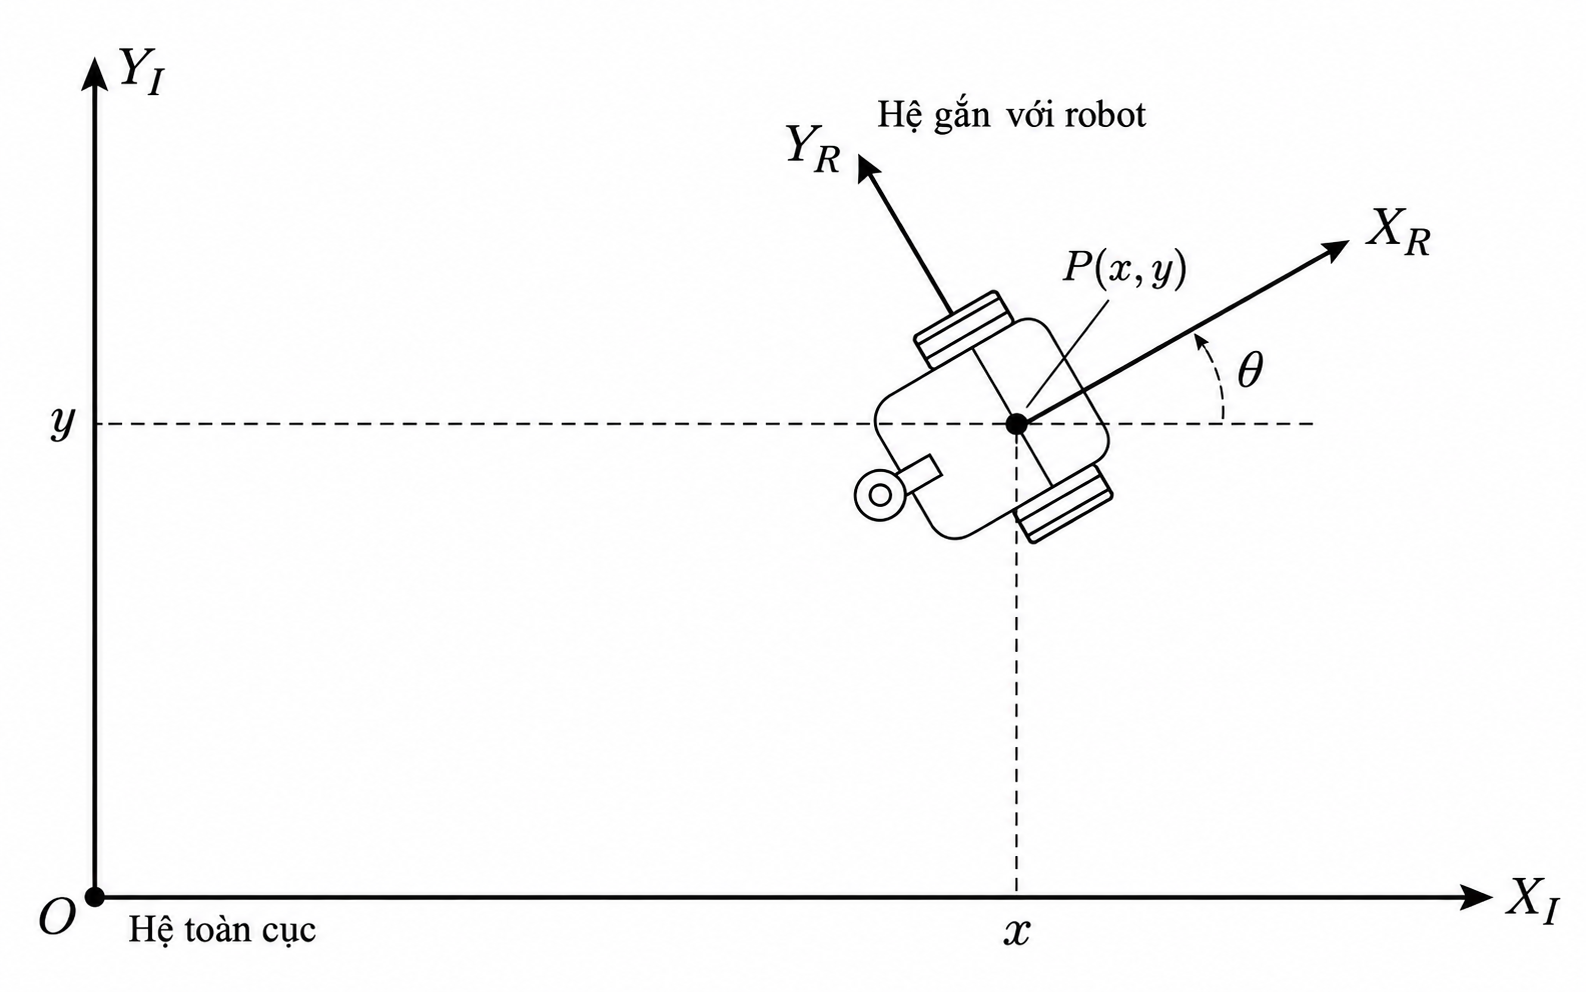
\includegraphics[width=0.8\linewidth]{he-toa-do-robot.png}
    \chuthichhinh[fig:he-toa-do-robot]{Hệ tọa độ toàn cục và hệ tọa độ gắn với thân robot}
    \end{minipage}
  \end{center}

Vector tư thế được dùng để xác định vị trí và hướng của robot trong hệ tọa độ toàn cục:
\[
  \xi_I=
  \begin{bmatrix}x\\y\\\theta\end{bmatrix}.
\]

Để chuyển từ hệ tọa độ toàn cục sang hệ tọa độ gắn với robot, sử dụng ma trận quay trực giao \(R(\theta)\) để ánh xạ các trục của hệ tọa độ toàn cục sang hệ tọa độ gắn liền robot:
\[
  R(\theta)=
  \begin{bmatrix}
    \cos\theta & \sin\theta & 0\\
    -\sin\theta & \cos\theta & 0\\
    0 & 0 & 1
  \end{bmatrix}.
\]

\subsection{Phương trình Động học Thuận (FK) và Động học Ngược (IK) của hệ xe vi sai 2 bánh chủ động + 1 bánh tự lựa (Caster Wheel).}

\subsubsection{Mô hình robot dẫn động vi sai (The Differential-Drive Robot)}

  \begin{center}
    \begin{minipage}{\linewidth}
    \centering
    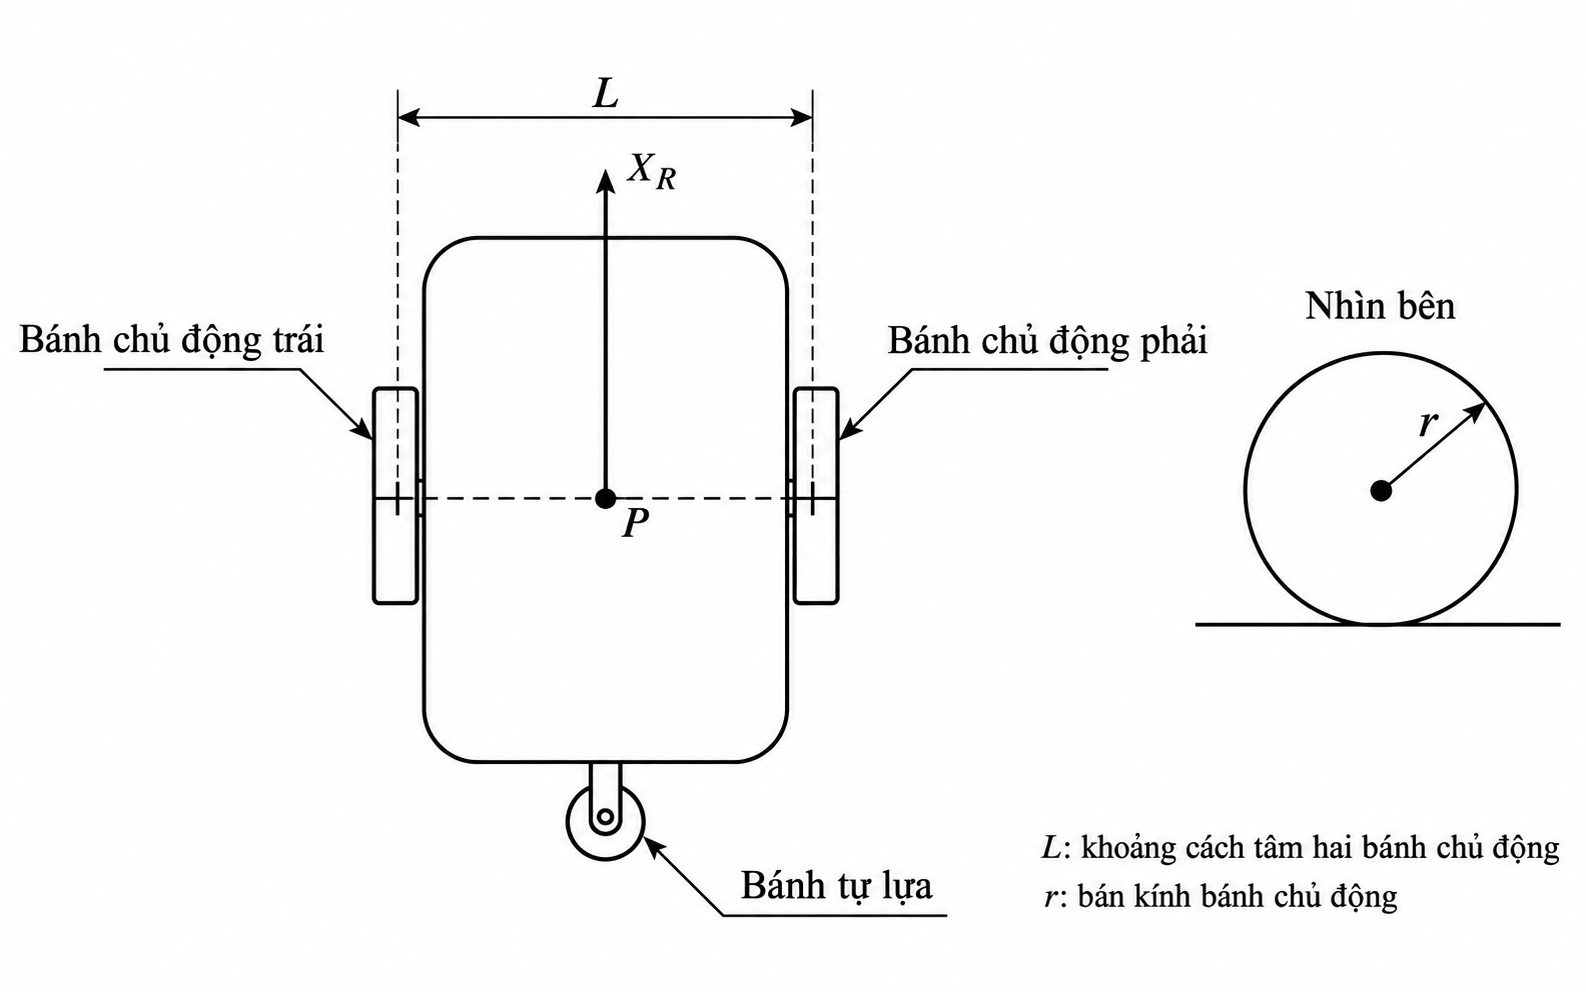
\includegraphics[width=0.8\linewidth]{robot-dan-dong-vi-sai.png}
    \chuthichhinh[fig:robot-vi-sai]{Mô hình robot dẫn động vi sai hai bánh chủ động}
    \end{minipage}
  \end{center}

Một hệ robot dẫn động vi sai bao gồm hai bánh xe đồng bán kính \(r\), khoảng cách giữa hai bánh chủ động là \(2d\), được dẫn động độc lập và quay quanh một trục chung, cùng với một hoặc nhiều bánh xe tự lựa (caster wheels), bánh xe dạng bi hoặc đế trượt ma sát thấp giúp giữ robot ở trạng thái cân bằng theo phương ngang.

Biểu diễn cấu hình của hệ dẫn động vi sai:
\[
  q=(\phi,x,y,\theta_L,\theta_R),
\]
với \(\theta_L\) và \(\theta_R\) lần lượt là góc quay của bánh xe bên trái và bên phải; \(\phi\) là góc hướng của thân robot, tương ứng với \(\theta\) trong biểu diễn tư thế ở mục 2.1.1.

\textbf{Ưu điểm:} Hệ đơn giản (thường động cơ được gắn trực tiếp vào trục của mỗi bánh xe) và có tính cơ động cao (robot có thể xoay tại chỗ bằng cách quay các bánh xe theo chiều ngược nhau). Tuy nhiên, bánh xe caster thường không phù hợp để dùng ngoài trời.

\subsubsection{Mô hình động học thuận của robot dẫn động vi sai}

Bài toán động học thuận cho biết vận tốc góc của hai bánh xe \((\omega_{\text{phải}},\omega_{\text{trái}})\), yêu cầu tính toán vận tốc ở tâm robot \((v,\omega)\) và sự thay đổi vị trí của robot trong không gian \((\dot{x},\dot{y},\dot{\theta})\).

Trong các công thức dưới đây, thống nhất ký hiệu \(r\) là bán kính bánh xe và \(L=2d\) là khoảng cách giữa hai bánh chủ động. Với quan hệ vận tốc dài của mỗi bánh xe bằng bán kính nhân vận tốc góc, ta có vận tốc tuyến tính của robot:
\[
  v=\frac{v_{\text{phải}}+v_{\text{trái}}}{2}
   =\frac{r(\omega_{\text{phải}}+\omega_{\text{trái}})}{2}.
\]

Vận tốc góc của robot:
\[
  \omega=\frac{v_{\text{phải}}-v_{\text{trái}}}{L}
        =\frac{r(\omega_{\text{phải}}-\omega_{\text{trái}})}{L}.
\]

Biểu diễn mối liên hệ giữa vận tốc bánh xe và vận tốc tâm robot:
\[
  \begin{bmatrix}v\\\omega\end{bmatrix}
  =\begin{bmatrix}
    \dfrac{r}{2} & \dfrac{r}{2}\\[6pt]
    \dfrac{r}{L} & -\dfrac{r}{L}
  \end{bmatrix}
  \begin{bmatrix}\omega_{\text{phải}}\\\omega_{\text{trái}}\end{bmatrix}.
\]

Chiếu lên hệ tọa độ toàn cục thu được phương trình động học thuận của robot vi sai dạng ma trận:
\[
  \begin{bmatrix}\dot{x}\\\dot{y}\\\dot{\theta}\end{bmatrix}
  =\begin{bmatrix}
    \dfrac{r}{2}\cos\theta & \dfrac{r}{2}\cos\theta\\[6pt]
    \dfrac{r}{2}\sin\theta & \dfrac{r}{2}\sin\theta\\[6pt]
    \dfrac{r}{L} & -\dfrac{r}{L}
  \end{bmatrix}
  \begin{bmatrix}\omega_{\text{phải}}\\\omega_{\text{trái}}\end{bmatrix}.
\]

\subsubsection{Mô hình động học nghịch của robot dẫn động vi sai}

Ngược với bài toán động học thuận, khi đã biết vận tốc góc và vận tốc tuyến tính của tâm robot, bài toán động học nghịch tính toán vận tốc góc của hai bánh xe.

Giải phương trình động học thuận, ta tìm được vận tốc dài của hai bánh xe:
\[
  v_{\text{phải}}=v+\frac{\omega L}{2},
  \qquad
  v_{\text{trái}}=v-\frac{\omega L}{2}.
\]

Với \(\omega_{\text{phải}}=v_{\text{phải}}/r\) và \(\omega_{\text{trái}}=v_{\text{trái}}/r\), ta tìm được vận tốc góc của hai bánh xe và biểu diễn phương trình dưới dạng ma trận:
\[
  \begin{bmatrix}\omega_{\text{phải}}\\\omega_{\text{trái}}\end{bmatrix}
  =\begin{bmatrix}
    \dfrac{1}{r} & \dfrac{L}{2r}\\[6pt]
    \dfrac{1}{r} & -\dfrac{L}{2r}
  \end{bmatrix}
  \begin{bmatrix}v\\\omega\end{bmatrix}.
\]

\subsubsection{Bánh tự lựa (Caster Wheel)}

  \begin{center}
    \begin{minipage}{\linewidth}
    \centering
    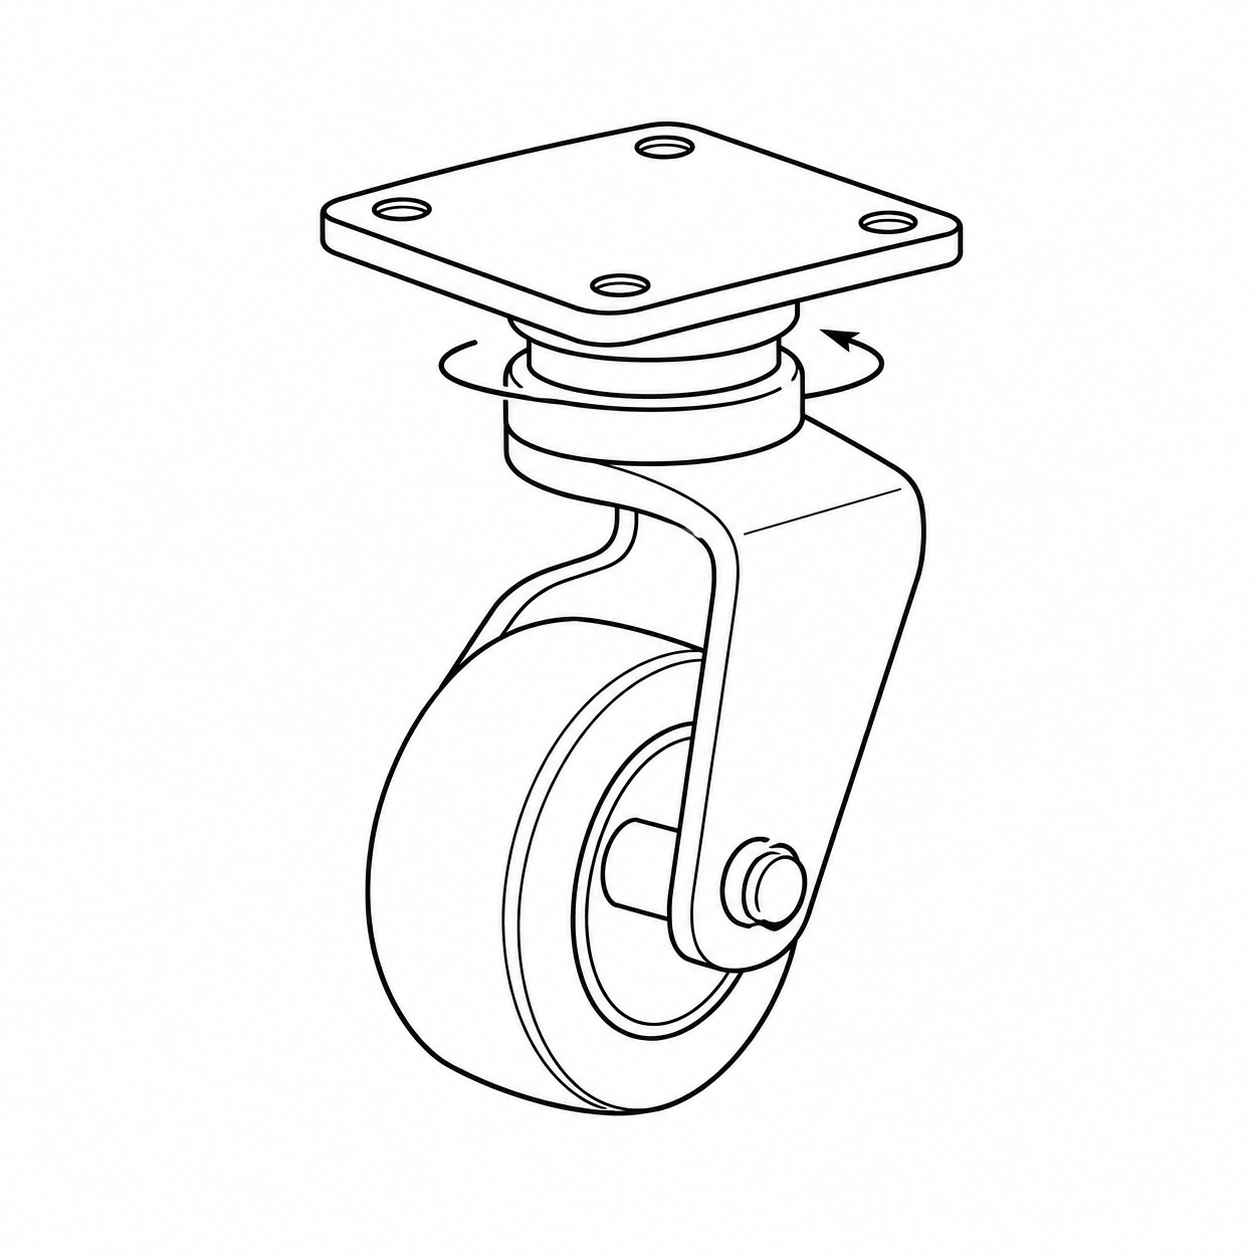
\includegraphics[width=0.3\linewidth]{banh-xe-tu-lua.png}
    \chuthichhinh[fig:banh-tu-lua]{Cấu tạo và các tham số hình học của bánh tự lựa}
    \end{minipage}
  \end{center}

Bánh xe tự lựa có khả năng xoay quanh một trục thẳng đứng; trục quay này không đi qua điểm tiếp xúc của bánh xe với mặt đất. Tại điểm tiếp xúc với mặt đất (vị trí \(B\)), bánh xe được nối với trục quay thẳng đứng (vị trí \(A\)) thông qua một thanh cứng \(AB\) có chiều dài cố định là \(d\). Mặt phẳng của bánh xe luôn được duy trì thẳng hàng với đoạn \(AB\) trong mọi thời điểm. Ví dụ: bánh xe của ghế di động trong văn phòng.

Tương tự như bánh xe tiêu chuẩn bẻ lái được, bánh xe tự lựa có hai tham số biến thiên theo thời gian: góc quay \(\varphi(t)\) của bánh xe và góc lái \(\beta(t)\), hay hướng của thanh nối \(AB\). Trong hình học bánh tự lựa, \(l\) là khoảng cách từ điểm tham chiếu \(P\) đến điểm gắn \(A\), \(\alpha\) xác định hướng của đoạn \(PA\), \(d\) là độ lệch \(AB\) và \(r\) là bán kính bánh tự lựa. Các ký hiệu hình học này được xét riêng cho bánh tự lựa.

\textbf{Phương trình ràng buộc lăn (rolling constraint):}
\[
  \begin{bmatrix}
    \sin(\alpha+\beta) & -\cos(\alpha+\beta) & -l\cos\beta
  \end{bmatrix}
  R(\theta)\dot{\xi}_I-r\dot{\varphi}=0.
\]

\textbf{Phương trình ràng buộc trượt (sliding constraint):}
\[
  \begin{bmatrix}
    \cos(\alpha+\beta) & \sin(\alpha+\beta) & d+l\sin\beta
  \end{bmatrix}
  R(\theta)\dot{\xi}_I+d\dot{\beta}=0.
\]

Cấu trúc hình học của bánh xe tự lựa ảnh hưởng lớn đến sliding constraint vì lực ngang tác dụng lên bánh xe xảy ra tại điểm gắn bánh xe với khung robot (điểm \(A\)) thay vì tại điểm tiếp xúc với mặt đất. Sự chênh lệch vị trí này khiến cho giả định về việc chuyển động ngang bằng \(0\) trở nên sai lệch. Vì vậy, bất kỳ chuyển động nào vuông góc với mặt phẳng bánh xe đều phải được bù bằng một chuyển động xoay tương ứng của trục thẳng đứng.

\subsection{\texorpdfstring{Phân tích Ràng buộc Phi Holonomic(\(\dot{y}\cos \theta -\dot{x}\sin \theta =0\)) và giới hạn bán kính quay vòng cực tiểu.}{Phân tích Ràng buộc Phi Holonomic(ycosθ-xsinθ=0) và giới hạn bán kính quay vòng cực tiểu.}}

\subsubsection{Tính holonomic của robot}

Tính holonomic (hay tính toàn phương / tính ràng buộc tích phân được) được sử dụng để mô tả không gian quỹ đạo của robot di động. Trong nghiên cứu robot di động, thuật ngữ này bao gồm các ràng buộc động học của khung robot.

Có thể hiểu tính holonomic của robot mô tả mối quan hệ giữa số bậc tự do có thể điều khiển trực tiếp và tổng số bậc tự do của không gian cấu hình C-space.

Robot holonomic là robot không có bất kỳ ràng buộc phi holonomic (non-holonomic) nào. Ngược lại, robot phi holonomic là robot có một hoặc nhiều ràng buộc động học phi holonomic.

Robot bao gồm hệ vi sai hai bánh sau và một bánh caster tự lựa ở phía trước được phân loại là hệ phi holonomic.

\subsubsection{Tính chất của ràng buộc phi holonomic của robot}

Các phương trình biểu diễn ràng buộc phi holonomic yêu cầu mối quan hệ vi phân giữa các biến vị trí (ví dụ như đạo hàm của \(x\) và \(y\)). Các ràng buộc này không thể lấy tích phân để đưa về quan hệ chỉ phụ thuộc vào các biến cấu hình.

Phương trình
\[
  \dot{y}\cos\theta-\dot{x}\sin\theta=0
\]
là biểu thức ràng buộc không trượt ngang của bánh xe. Vector vận tốc của robot phải có phương trùng với trục dọc của nó trong hệ tọa độ thân robot; robot không thể di chuyển theo phương vuông góc với hướng đang chỉ định.

Phương trình \(\dot{y}\cos\theta-\dot{x}\sin\theta=0\) không thể lấy tích phân thành dạng \(f(x,y,\theta)=0\) để có một phương trình đại số biểu diễn liên hệ giữa các đại lượng trong hệ tọa độ Đề-các \(x,y,\theta\). Vì vậy, theo tính chất, hệ này là hệ phi holonomic.

Ràng buộc này giới hạn số bậc tự do của không gian vận tốc (velocity space), nhưng không làm giảm số bậc tự do của không gian cấu hình. Đồng nghĩa với việc robot vẫn có thể đi tới bất kỳ tọa độ \((x,y,\theta)\) nào trong mặt phẳng, nhưng phải thực hiện bằng các chuỗi thao tác kết hợp (tiến, lùi, rẽ hướng).

\subsubsection{\texorpdfstring{Giới hạn bán kính quay vòng cực tiểu \(R_{\mathrm{min}}\)}{Giới hạn bán kính quay vòng cực tiểu Rmin}}

Công thức bán kính quay vòng đối với robot dẫn động vi sai:
\[
  R=\frac{v}{\omega}
   =\frac{L(v_{\text{phải}}+v_{\text{trái}})}
           {2(v_{\text{phải}}-v_{\text{trái}})},
  \qquad \omega\neq 0.
\]
Với \(v=(v_{\text{phải}}+v_{\text{trái}})/2\) và \(\omega=(v_{\text{phải}}-v_{\text{trái}})/L\) là vận tốc dài và vận tốc góc của robot, \(L\) là khoảng cách giữa hai bánh xe chủ động; \(v_{\text{phải}}\) và \(v_{\text{trái}}\) là vận tốc của bánh phải và bánh trái.

Khi điều khiển hai bánh xe có vận tốc bằng nhau về độ lớn nhưng ngược chiều nhau, \(v_{\text{phải}}=-v_{\text{trái}}\neq 0\), hai bánh xe quay ngược chiều nhau và xe sẽ tự quay vòng tròn quanh tâm của trục nối hai bánh. Như vậy, \(v_{\text{phải}}+v_{\text{trái}}=0\), kéo theo \(R=0\). Do đó, bán kính quay vòng cực tiểu xét về độ lớn là
\[
  R_{\mathrm{min}}=0.
\]

\textbf{Hệ quả:} Thao tác quay đầu tại chỗ mang lại sự linh hoạt cho robot, giúp việc hoạch định quỹ đạo đơn giản hơn do không có giới hạn bán kính quay tối thiểu dương trong mô hình động học lý tưởng.

\section{\texorpdfstring{Ràng buộc Vật lý và Điều kiện Liên tục của Quỹ đạo (\(C^{0},C^{1},C^{2},C^{3}\))}{Ràng buộc Vật lý và Điều kiện Liên tục của Quỹ đạo (C0,C1,C2,C3)}}

\subsection{\texorpdfstring{Ý nghĩa vật lý của Vị trí (\(q\)), Vận tốc (\(\dot{q}\)), Gia tốc (\(\ddot{q}\)) và Độ giật (\(Jerk-\dddot{q}\)).}{Ý nghĩa vật lý của Vị trí (q), Vận tốc (q), Gia tốc (q) và Độ giật (Jerk-q).}}

\begin{itemize}
  \item \textbf{Vị trí \(q\):} Cho biết tọa độ trong không gian hoặc trạng thái không gian của robot ở một thời điểm nhất định. Trong cấu hình của robot, \(q\) có thể được biểu diễn bằng tọa độ Đề-các \((x,y,z)\); \(q\) cũng có thể biểu diễn góc quay \(\theta\) của các khớp hoặc độ dịch chuyển tịnh tiến. Tập hợp các giá trị \(q\) xác định hoàn toàn trạng thái tĩnh của hệ thống trong không gian cấu hình (configuration space).
  \item \textbf{Vận tốc \(\dot{q}\):} Là đạo hàm bậc 1 của vị trí theo biến thời gian. Vận tốc cho biết tốc độ thay đổi vị trí của robot trong hệ tọa độ toàn cục, cho biết robot đang di chuyển nhanh hay chậm, theo hướng nào. \textbf{Ứng dụng:} Tính toán tốc độ của robot hoặc tốc độ quay của động cơ để hoàn thành quãng đường di chuyển trong thời gian được yêu cầu.
  \item \textbf{Gia tốc \(\ddot{q}\):} Là đạo hàm bậc 2 của vị trí theo biến thời gian. Gia tốc cho biết tốc độ thay đổi của vận tốc theo thời gian. Gia tốc tỷ lệ thuận với lực hoặc mô-men xoắn tác động lên robot theo định luật II Newton (\(F=ma\), \(\tau=I\alpha\)). Gia tốc quyết định lực hoặc mô-men tối đa mà các cơ cấu chấp hành như động cơ cần cung cấp để robot di chuyển. Ngoài ra, để động cơ không bị quá tải, có thể khống chế gia tốc.
  \item \textbf{Độ giật \(\dddot{q}\):} Là đạo hàm bậc 3 của vị trí theo biến thời gian. Độ giật là tốc độ thay đổi của gia tốc theo thời gian. Vì liên quan đến lực nên độ giật biểu thị sự thay đổi đột ngột của lực tác động.
\end{itemize}

\textbf{Ứng dụng của việc kiểm soát độ giật:} Trong quy hoạch quỹ đạo, nếu độ giật lớn thì lực tác động thay đổi đột ngột, gây hiện tượng giật cục, rung lắc, kích thích các tần số cộng hưởng trong hệ thống, gây hao mòn robot và phá hủy cơ cấu cơ học.

Việc kiểm soát tốt độ giật giúp tạo ra các quỹ đạo mượt, robot vận hành êm ái và giảm thiểu sai số.

\subsection{\texorpdfstring{Tác động của gián đoạn gia tốc (\(C^{2}\)) và độ giật (\(C^{3}\)) đến hiện tượng trượt bánh xe, quá tải dòng điện động cơ và rung lắc khung gầm.}{Tác động của gián đoạn gia tốc (C2) và độ giật (C3) đến hiện tượng trượt bánh xe, quá tải dòng điện động cơ và rung lắc khung gầm.}}

Tính liên tục của các hàm đạo hàm theo biến thời gian sẽ quyết định độ mượt của quỹ đạo. Lớp liên tục (Continuity Class) \(C^{2}\) thể hiện tính liên tục của hàm gia tốc \(\ddot{q}(t)\), và \(C^{3}\) là tính liên tục của hàm độ giật \(\dddot{q}(t)\).

\begin{itemize}
  \item \textbf{Gián đoạn gia tốc:} Quỹ đạo chuyển động không thỏa mãn độ liên tục bậc 2 \(C^{2}\). Đồ thị gia tốc sẽ có dạng bước nhảy (thay đổi đột ngột từ mức này sang mức khác).
  \item Quỹ đạo chỉ đạt độ liên tục lớp \(C^{1}\) (vận tốc liên tục) và bị gián đoạn ở đạo hàm bậc 2; độ giật tại điểm gián đoạn được mô tả bằng xung lý tưởng có độ lớn vô hạn, gây hại đến robot.
\end{itemize}

\subsubsection{Hiện tượng trượt bánh xe (wheel slipping)}

Khi robot di chuyển, lực ma sát nghỉ cực đại giữa bánh xe và bề mặt là
\[
  F_{\mathrm{msn}}=\mu N,
\]
trong đó \(\mu\) là hệ số ma sát của bề mặt, \(N\) là phản lực của bề mặt lên robot. Lực kéo hay lực tiếp tuyến là
\[
  F_k=m\ddot{q}=ma.
\]

Khi có gián đoạn gia tốc xảy ra, tính liên tục lớp \(C^{2}\) không được đảm bảo; giá trị gia tốc của hệ thống đột ngột thay đổi khiến \(F_k\) cũng đột ngột tăng lên. Nếu lực kéo \(F_k\) vượt quá giới hạn lực ma sát nghỉ \(F_{\mathrm{msn}}\) giữa bánh xe và mặt sàn, hiện tượng trượt bánh xe xảy ra.

\textbf{Hệ quả:} Bánh xe chuyển sang chịu ma sát trượt thay vì lăn không trượt, gây xoay tít bánh xe, ảnh hưởng đến hệ thống định vị vi sai.

\subsubsection{Quá tải dòng điện động cơ}

Mô-men xoắn đầu ra của động cơ tỷ lệ thuận với dòng điện qua cuộn dây. Phương trình liên hệ giữa dòng điện trong cuộn dây và độ giật:
\[
  \frac{di}{dt}=\frac{I_m}{K_t}\,\dddot{q}(t).
\]
Trong đó, \(I_m\) là mô-men quán tính và \(K_t\) là hằng số mô-men của động cơ; quan hệ trên được xét cho chuyển động quay với \(q\) là góc quay trong mô hình quán tính đơn giản.

Khi có gián đoạn gia tốc, độ giật \(\dddot{q}\) tiến tới vô hạn trong mô hình lý tưởng, kéo theo độ biến thiên dòng điện tăng đến rất lớn. Trên đồ thị dòng điện sẽ xuất hiện các đỉnh nhọn.

\textbf{Hệ quả:} Sụt áp trên nguồn điện như pin, ắc quy; khiến vi điều khiển bị treo hoặc tự reset; tăng tổn hao nhiệt lên mức gây hại; trực tiếp ngắt robot bởi cơ chế bảo vệ quá dòng.

\subsubsection{Rung lắc khung gầm}

Độ mềm dẻo cơ học của khung gầm khiến nó dễ dàng bị dao động cưỡng bức bởi độ giật vô hạn trong mô hình lý tưởng của robot khi gia tốc bị gián đoạn.

Dao động của khung gầm có dải tần số rộng, kích thích tần số dao động riêng của hệ thống cơ khí, gây ra hiện tượng cộng hưởng cơ học.

\textbf{Hệ quả:} Làm xuất hiện dao động thừa khi robot hoàn thành bước di chuyển; gây nhiễu tín hiệu lên các cảm biến nhạy cảm, làm giảm độ chính xác của thuật toán; gây mỏi cơ khí.

% Trở lại độ sâu đánh số của phần tài liệu đã có.
\setcounter{secnumdepth}{2}

\section{Các Phương pháp Tạo Profile Vận tốc 1D (Trajectory Generation)}

\subsection{Phương pháp Nội suy Đa thức Bậc 3 (Cubic) và Đa thức Bậc 5 (Quintic Polynomial) qua các điểm nút vị trí - thời gian.}

\subsubsection*{a. Mô hình động lực học của xe.}

\[
M\left( q \right)\ddot{q}+C\left( q,\dot{q} \right)\dot{q}+G\left( q \right)=\tau 
\]

Trong đó:

Tín hiệu đầu ra\textbf{:} \(y=q\) (tọa độ vị trí / góc quay của khớp).

Tín hiệu đầu vào: \(u=\tau \) (mô-men hoặc lực điều khiển cấp vào khớp).

Khi biến đổi sang hệ phương trình trạng thái phi tuyến, ta áp dụng quy tắc đặt biến trạng thái.

\[
\left\{ \begin{matrix}
x_{1}=q \\ x_{2}=\dot{q}
\end{matrix} \right.
\]

Lấy đạo hàm cấp 1 theo thời gian của các biến trạng thái:

\[
\left\{ \begin{matrix}
\dot{x}_{1}=\dot{q}=x_{2} \\ \dot{x}_{2}=\ddot{q}=M^{-1}\left( x_{1} \right)\left[ u-C\left( x_{1},x_{2} \right)x_{2}-G\left( x_{1} \right) \right]
\end{matrix} \right.
\]

Phương trình đầu ra:

\[
y=x_{1}
\]

\subsubsection*{b. Mối quan hệ với lý thuyết điều khiển tự động.}

\[
y^{\left( n \right)}+a_{n-1}y^{\left( n-1 \right)}+\dots +a_{1}\dot{y}+a_{0}y=b_{0}u\left( t \right)
\]

Quy tắc đặt biến: Đặt tuần tự các biến trạng thái bằng chính các đạo hàm của biến đầu ra y:

\[
\left\{ \begin{matrix}
\dot{x}_{1}=x_{2} \\ \dot{x}_{2}=x_{3} \\ \vdots  \\ \dot{x}_{n}=-a_{0}x_{1}-a_{1}x_{2}-\dots -a_{n-1}x_{n}+b_{0}u\left( t \right)
\end{matrix} \right.
\]

Dạng ma trận 
\[
\left\{ \begin{matrix}
\dot{x}=Ax+Bu \\ y=Cx
\end{matrix} \right.
\]

\subsection{Profile Vận tốc Hình thang (Trapezoidal / LSPB Profile) — Khai triển hệ phương trình phân đoạn gia tốc - đều - giảm tốc.}

\subsubsection*{a. Khái niệm}

Profile vận tốc hình thang là quy luật quỹ đạo 1D chia toàn bộ quá trình dịch chuyển từ \(q_{0}\) đến \(q_{f}\), trong khoảng thời gian \(t\in \left[ 0,t_{f} \right]\) thành 3 giai đoạn nối tiếp nhau: Tăng tốc, gia tốc không đổi, và gả, tốc.

\subsubsection*{b. Khai triển}

Giả sử: xuất phát và kết thúc tại trạng thái nghỉ (\(v_{0}=0\) tại \(t=0\); \(v_{f}=0\) tại \(t=t_{f}\)).

\subsubsection*{Giai đoạn 1: Tăng tốc đều (\(0\leq t\leq t_{b}\))}

Ở pha này, gia tốc được duy trì ở mức cực đại hằng số, làm vận tốc tăng tuyến tính và vị trí biến thiên theo dạng hàm bậc hai:

\[
\ddot{q}\left( t \right)=a
\]

\[
\dot{q}\left( t \right)=at
\]

\[
q\left( t \right)=q_{0}+\frac{1}{2}at^{2}
\]

Tại điểm kết thúc pha tăng tốc \(t=t_{b}\):

- Vận tốc đạt đỉnh: \(V=\dot{q}\left( t_{b} \right)=at_{b}\).

- Vị trí trung gian: \(q\left( t_{b} \right)=q_{0}+\frac{1}{2}at_{b}^{2}=q_{0}+\frac{1}{2}Vt_{b}\).

\subsubsection*{Giai đoạn 2: Chuyển động đều (\(t_{b}<t\leq t_{f}-t_{b}\))}

Gia tốc triệt tiêu hoàn toàn, hệ thống vận hành với vận tốc hằng V, quỹ đạo vị trí là một đường thẳng tuyến tính theo thời gian:

\[
\ddot{q}\left( t \right)=0
\]

\[
\dot{q}\left( t \right)=V
\]

Tích phân vận tốc từ điều kiện biên vị trí liên tục tại \(t=t_{b}\):

\[
q\left( t \right)=q\left( t_{b} \right)+\int_{t_{b}}^{t} V\,d\tau =q\left( t_{b} \right)+V\left( t-t_{b} \right)
\]

Thay \(q\left( t_{b} \right)=q_{0}+\frac{1}{2}at_{b}^{2}\) vào biểu thức:

\[
q\left( t \right)=q_{0}+\frac{1}{2}at_{b}^{2}+Vt-Vt_{b}
\]

Vì \(V=at_{b}\Longrightarrow \frac{1}{2}at_{b}^{2}-Vt_{b}=-\frac{1}{2}at_{b}^{2}=-\frac{1}{2}Vt_{b}\), phương trình vị trí được rút gọn thành:

\[
q\left( t \right)=q_{0}-\frac{1}{2}at_{b}^{2}+Vt
\]

\subsubsection*{Giai đoạn 3: Giảm tốc đều (\(t_{f}-t_{b}<t\leq t_{f}\))}

Hệ thống hãm phanh với gia tốc không đổi mang dấu âm (\(-a\)), vận tốc giảm tuyến tính về 0 tại \(t=t_{f}\), và vị trí uốn cong theo nhánh parabol ngược để tiệm cận êm tới tọa độ đích \(q_{f}\):

\[
\ddot{q}\left( t \right)=-a
\]

\[
\dot{q}\left( t \right)=a\left( t_{f}-t \right)
\]

\[
q\left( t \right)=q_{f}-\frac{1}{2}a{\left( t_{f}-t \right)}^{2}
\]

\subsection{Profile Vận tốc Đường cong chữ S (S-Curve 7 đoạn) — Giải thuật kiểm soát và triệt tiêu xung Jerk.}

Trong kỹ thuật điều khiển chuyển động chính xác cao, hạn chế lớn nhất của profile vận tốc hình thang (Trapezoidal / LSPB) là gia tốc biến thiên đột ngột dạng hàm bước nhảy, làm phát sinh xung độ giật vô hạn (\(j\left( t \right)=\frac{da}{dt}\to \pm \infty \)) tại các mốc chuyển pha. Độ giật vô hạn này gây xung mô-men tác động trực tiếp lên hộp giảm tốc, kích thích rung động tự do của khung gầm và gây trượt vi sai bánh xe.

Profile đường cong chữ S (S-Curve / Jerk-bounded profile) giải quyết triệt để vấn đề này bằng cách khống chế độ giật trong một ngưỡng giới hạn vật lý định mức \(|j\left( t \right)|\leq j_{\mathrm{max}}\), từ đó đảm bảo gia tốc biến thiên liên tục, quỹ đạo đạt cấp mượt động học \(C^{2}\).

\subsubsection*{1. Cấu trúc 7 Pha Động học của Profile Chữ S}

Quá trình chuyển động từ vị trí xuất phát \(q_{0}\) đến đích \(q_{f}\) ở trạng thái nghỉ (\(v_{0}=v_{f}=0\)) được phân rã thành 7 giai đoạn giải tích nối tiếp nhau:

% TODO: Thay khung dưới bằng hình gia tốc a(t) và vận tốc v(t) của S-Curve.
% Sơ đồ ký tự trong bản Word được giữ trong các dòng chú thích bên dưới.

%       Gia tốc a(t)                            Vận tốc v(t)

%           ▲                                       ▲

%    +a_max ┼───┐  (Pha 2)                   v_max  ┼──────────┐ (Pha 4)

%           │  / \                                  │        .´ │`.

%           │ /   \                                 │      .´   │  `.

%         0 ┼/─────\─────────/─────\──► t         0 ┼─────´─────┴────`──► t

%           │ (1)  (3)      /  (5)  \               │   (Pha 1-3)  (Pha 5-7)

%   -a_max  │              └───┬─────┘              └─────────────────────►

%           ▼                (Pha 6)

% Khi có ảnh, thay khung trên bằng:
  \begin{figure}[htbp]
    \centering
    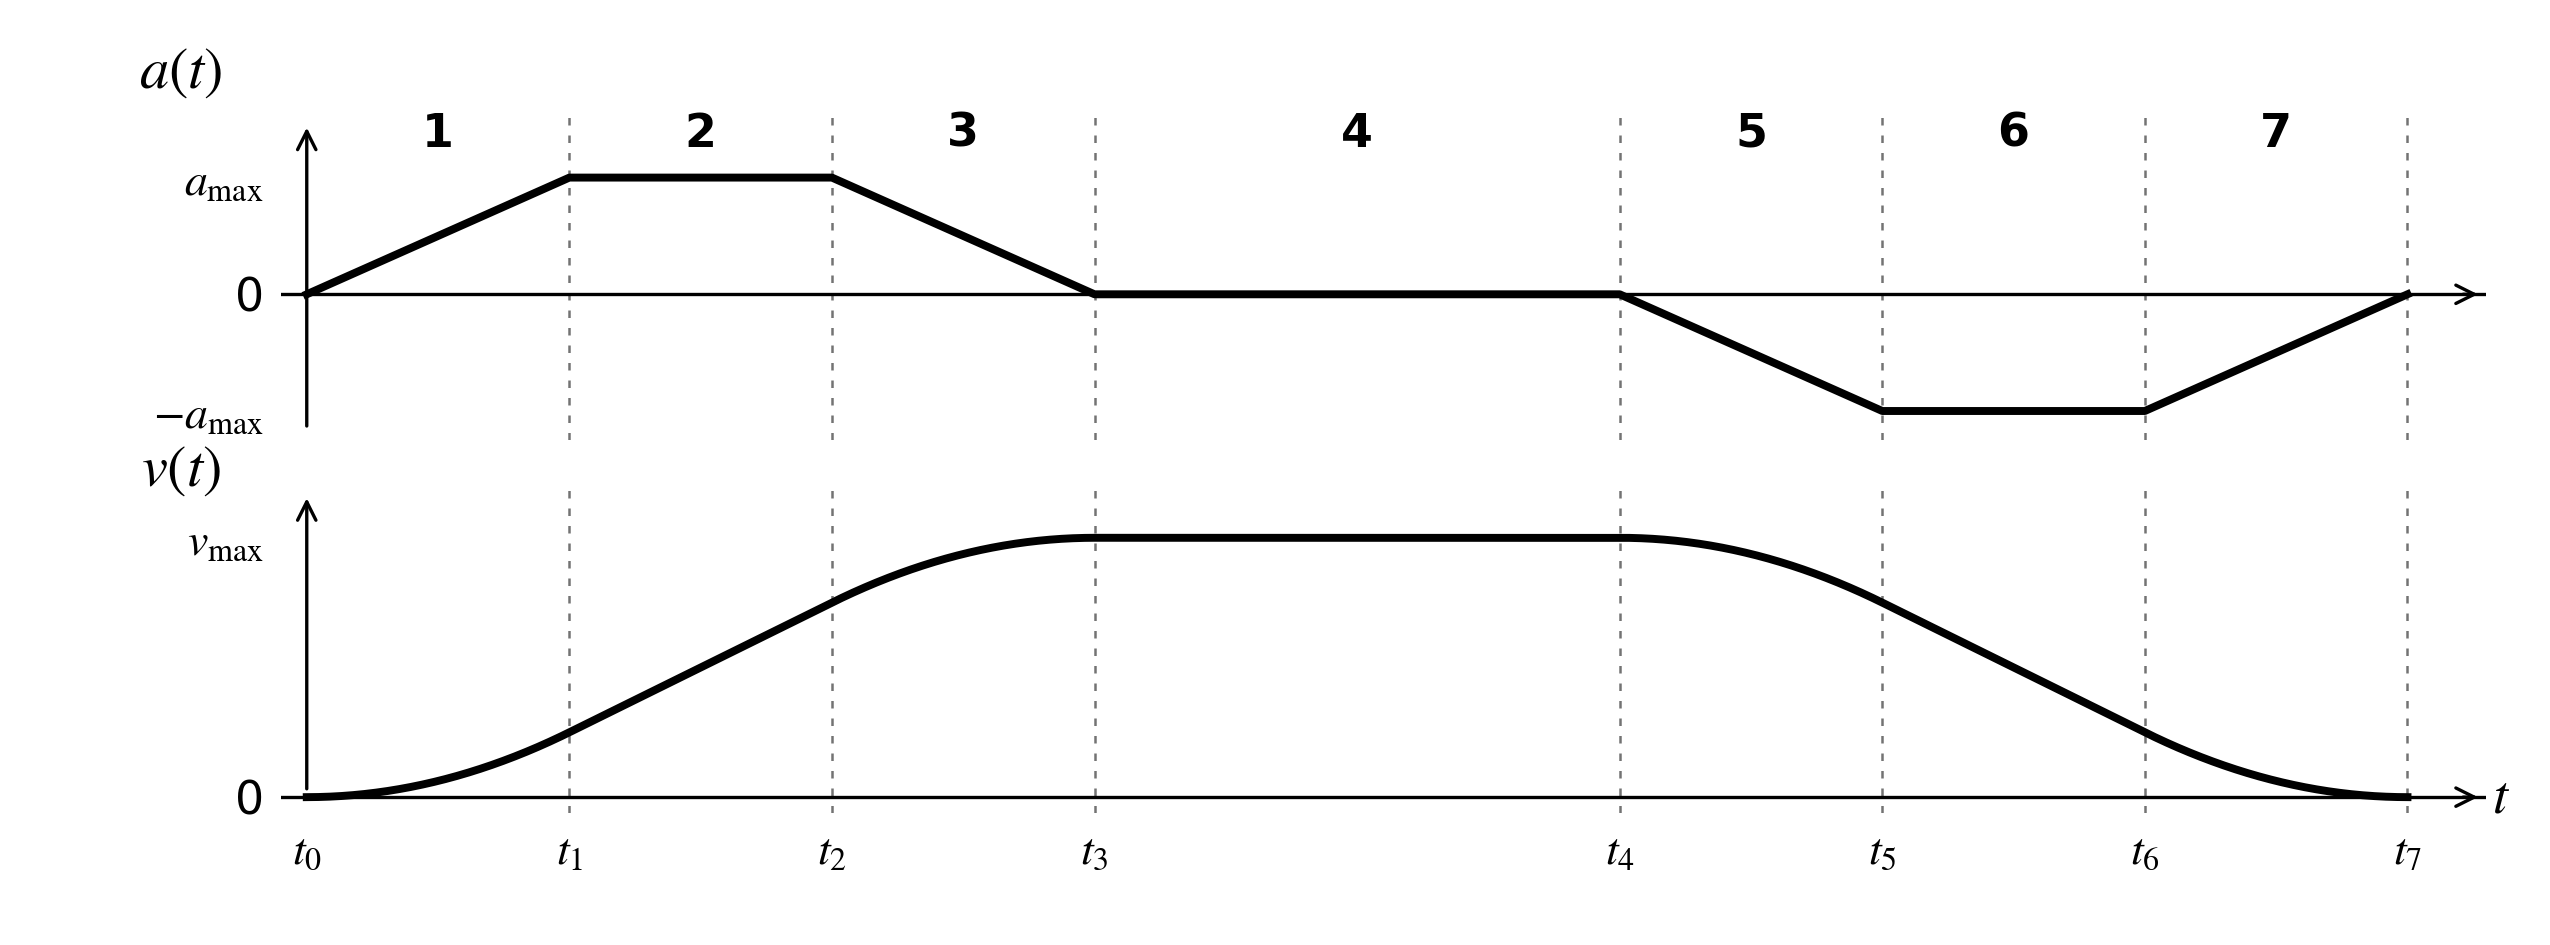
\includegraphics[width=0.95\linewidth]{s-curve.png}
    \caption{Gia tốc và vận tốc của profile chữ S.}
    \label{fig:s-curve}
  \end{figure}

\begin{itemize}

\item \textbf{Pha 1: Tăng gia tốc (Jerk dương hằng số} \(+j_{\mathrm{max}}\)\textbf{):} Gia tốc tăng tuyến tính từ \(0\) lên \(+a_{\mathrm{max}}\), làm vận tốc bắt đầu uốn cong parabol hướng lên.

\item \textbf{Pha 2: Gia tốc hằng (}\(j=0\)\textbf{):} Duy trì gia tốc cực đại \(+a_{\mathrm{max}}\), vận tốc tăng tuyến tính theo thời gian.

\item \textbf{Pha 3: Giảm gia tốc (Jerk âm hằng số} \(-j_{\mathrm{max}}\)\textbf{):} Gia tốc giảm tuyến tính từ \(+a_{\mathrm{max}}\) về \(0\), vận tốc tiệm cận mượt mà tới vận tốc danh định \(v_{\mathrm{max}}\).

\item \textbf{Pha 4: Chuyển động đều (}\(j=0,a=0\)\textbf{):} Hệ thống duy trì vận tốc không đổi \(v_{\mathrm{max}}\), gia tốc triệt tiêu hoàn toàn.

\item \textbf{Pha 5: Bắt đầu hãm phanh (Jerk âm hằng số} \(-j_{\mathrm{max}}\)\textbf{):} Gia tốc âm xuất hiện và giảm dần từ \(0\) xuống \(-a_{\mathrm{max}}\), vận tốc bắt đầu uốn cong hướng xuống.

\item \textbf{Pha 6: Giảm tốc hằng (}\(j=0\)\textbf{):} Duy trì hãm phanh với gia tốc âm không đổi \(-a_{\mathrm{max}}\), vận tốc giảm tuyến tính.

\item \textbf{Pha 7: Triệt tiêu gia tốc (Jerk dương hằng số} \(+j_{\mathrm{max}}\)\textbf{):} Gia tốc tăng từ \(-a_{\mathrm{max}}\) về lại \(0\), đưa vận tốc tiệm cận êm ái về \(0\) tại đúng tọa độ đích \(q_{f}\).

\end{itemize}

\subsubsection*{2. Khai triển Toán học Từng Giai đoạn}

Việc xây dựng profile chữ S được thực hiện từ quy luật biến thiên của độ giật, sau đó xác định lần lượt gia tốc, vận tốc và vị trí. Thay vì làm gia tốc thay đổi tức thời, phương pháp này dành một khoảng thời gian chuyển tiếp để tăng hoặc giảm gia tốc. Cấu trúc bảy pha vì vậy thể hiện cách tổ chức quá trình khởi động, di chuyển và dừng theo một quy luật có kiểm soát \cite[Mục 9.1--9.2]{lynch-park-modern-robotics}.

Trong trường hợp đối xứng đang xét, robot bắt đầu và kết thúc ở trạng thái nghỉ, gia tốc tại hai đầu bằng không, đồng thời sử dụng cùng giới hạn gia tốc và độ giật cho quá trình tăng tốc và giảm tốc. Gọi \(T_j\) là thời gian của mỗi pha thay đổi gia tốc, \(T_a\) là thời gian duy trì gia tốc dương không đổi và \(T_v\) là thời gian chuyển động đều. Thời gian duy trì gia tốc âm, ký hiệu \(T_d\), bằng \(T_a\) theo giả thiết đối xứng. Tổng thời gian chuyển động được viết gọn thành
\[
  T=4T_j+2T_a+T_v.
\]
Quan hệ này cho thấy thời gian hành trình gồm bốn khoảng chuyển tiếp gia tốc, hai khoảng duy trì gia tốc và một khoảng chuyển động đều. Một số khoảng có thể bằng không nếu quãng đường hoặc giới hạn vận tốc không cho phép hình thành đầy đủ cả bảy pha.

Về mặt toán học, gia tốc được xác định bằng cách tích phân độ giật; tiếp tục tích phân gia tốc thu được vận tốc và tích phân vận tốc thu được vị trí. Mỗi pha bắt đầu từ vị trí, vận tốc và gia tốc ở cuối pha trước. Cách kế thừa điều kiện biên này bảo đảm các đoạn chuyển động nối tiếp nhau, tránh việc đặt lại vận tốc hoặc gia tốc khi đổi pha.

Trong ba pha đầu, robot chuyển từ trạng thái nghỉ sang trạng thái chạy ổn định. Ở pha thứ nhất, độ giật dương làm gia tốc tăng đều theo thời gian, khiến vận tốc tăng dần với mức tăng ngày càng lớn. Khi đạt mức gia tốc đã lựa chọn, hệ thống chuyển sang pha thứ hai và giữ gia tốc không đổi; khi đó vận tốc tăng tuyến tính. Đến pha thứ ba, độ giật đổi sang dấu âm để đưa gia tốc trở về không. Robot vẫn tăng vận tốc trong pha này, nhưng mức tăng nhỏ dần cho tới khi đạt vận tốc đỉnh của hành trình.

Pha thứ tư là khoảng chuyển động đều. Gia tốc và độ giật đều bằng không, vận tốc được giữ ổn định và vị trí thay đổi tuyến tính theo thời gian. Vận tốc đỉnh có thể bằng giới hạn cho phép khi quãng đường đủ dài. Nếu quãng đường ngắn, khoảng chuyển động đều có thể bị rút ngắn hoặc không xuất hiện; khi đó vận tốc đỉnh phải được lựa chọn phù hợp với quãng đường tăng tốc và hãm còn lại.

Ba pha cuối thực hiện quá trình giảm tốc theo trình tự đối xứng với ba pha đầu. Ở pha thứ năm, độ giật âm làm gia tốc chuyển dần từ không sang giá trị âm, nhờ đó robot bắt đầu giảm vận tốc một cách từ từ. Pha thứ sáu duy trì gia tốc âm không đổi để tiếp tục hãm. Trong pha thứ bảy, độ giật dương đưa gia tốc âm trở về không, đồng thời vận tốc giảm về không tại vị trí kết thúc đã xác định.

Nhìn theo dạng hàm, các pha có độ giật không đổi khác không tạo ra gia tốc tuyến tính, vận tốc bậc hai và vị trí bậc ba theo thời gian cục bộ. Các pha có gia tốc không đổi tạo ra vận tốc tuyến tính và vị trí bậc hai; riêng pha chuyển động đều có vị trí tuyến tính. Đặc điểm này cho phép biểu diễn toàn bộ hành trình bằng các đoạn đa thức bậc thấp, trong khi vẫn giữ được tính liên tục của vị trí, vận tốc và gia tốc tại các điểm nối.

\subsubsection*{3. Giải thuật Xác định Thông số Thời gian (Parameter Synthesis)}

Mục đích của việc xác định thông số thời gian là phân bố thời lượng cho từng pha sao cho robot hoàn thành đúng độ dịch chuyển mà không vượt các giới hạn vận tốc, gia tốc và độ giật. Các giá trị cực đại là giới hạn được phép sử dụng, không phải mức bắt buộc phải đạt trong mọi hành trình. Quãng đường càng ngắn thì khả năng đạt đồng thời các giới hạn này càng giảm.

Quy trình dưới đây xét chuyển động một chiều giữa hai trạng thái nghỉ, với gia tốc đầu và cuối bằng không, giới hạn tăng tốc và giảm tốc đối xứng. Độ dịch chuyển được xét theo độ lớn; chiều chuyển động được gán sau khi xác định quy luật. Nếu trạng thái ban đầu đang có vận tốc, hoặc khả năng tăng tốc và hãm khác nhau, việc phân bố thời gian cần được xây dựng lại theo các điều kiện biên tương ứng.

\subsubsection*{Bước 1: Kiểm tra khả năng đạt gia tốc cực đại \(a_{\mathrm{max}}\)}

Trước hết, cần xác định liệu robot có thể tăng gia tốc tới giới hạn cho phép rồi đưa gia tốc trở về không mà vẫn giữ vận tốc trong giới hạn hay không. Thời gian chuyển tiếp phụ thuộc vào tốc độ thay đổi gia tốc được cho phép: giới hạn độ giật càng nhỏ thì quá trình hình thành cùng một mức gia tốc càng kéo dài.

Nếu giới hạn vận tốc đủ lớn, robot có thể đạt gia tốc cực đại và duy trì mức này trong một khoảng thời gian trước khi giảm gia tốc về không. Khoảng duy trì được lựa chọn theo phần vận tốc còn cần tích lũy sau hai pha chuyển tiếp. Trong trường hợp biên, robot chỉ vừa chạm mức gia tốc cực đại rồi chuyển ngay sang giảm gia tốc, không có khoảng duy trì riêng.

Nếu giới hạn vận tốc thấp, robot có thể tích lũy đủ vận tốc ngay khi gia tốc còn chưa đạt giá trị cực đại. Khi đó, cần giảm gia tốc đỉnh và bỏ pha duy trì gia tốc hằng. Theo giả thiết đối xứng, pha duy trì giảm tốc hằng ở nửa sau hành trình cũng được loại bỏ. Profile vẫn giữ các khoảng tăng và giảm gia tốc có kiểm soát, nhưng số pha có thời lượng khác không ít hơn bảy.

Kết quả của bước này là một phương án tăng tốc và giảm tốc dự kiến để đạt giới hạn vận tốc mà không vi phạm giới hạn gia tốc, độ giật. Đây mới là kiểm tra theo các giới hạn chuyển động; phương án còn phải được đối chiếu với quãng đường thực tế ở bước tiếp theo.

\subsubsection*{Bước 2: Kiểm tra khả năng đạt vận tốc cực đại \(v_{\mathrm{max}}\)}

Sau khi xác định các khoảng tăng tốc và giảm tốc dự kiến, cần tính phần quãng đường mà hai quá trình này sử dụng. Nếu độ dịch chuyển yêu cầu lớn hơn phần quãng đường đó, robot có thể đạt vận tốc cực đại và dành quãng đường còn lại cho chuyển động đều. Thời lượng pha chuyển động đều được xác định từ quãng đường còn lại và vận tốc duy trì.

Nếu quãng đường yêu cầu vừa đủ cho tăng tốc và hãm, robot chỉ đạt vận tốc đỉnh tại thời điểm chuyển tiếp giữa hai quá trình, không có pha chạy đều. Nếu quãng đường ngắn hơn, vận tốc đỉnh phải được giảm xuống để robot vẫn dừng đúng vị trí đích. Việc giảm tốc cần được tính ngay từ khi lập quỹ đạo, bởi quá trình hãm cũng bao gồm thời gian hình thành và giải phóng gia tốc âm.

Khi phải giảm vận tốc đỉnh, có hai dạng chuyển động cần phân biệt. Với quãng đường còn tương đối lớn, robot vẫn có thể đạt gia tốc cực đại nhưng thời gian duy trì gia tốc được rút ngắn. Với quãng đường rất ngắn, robot không đạt cả gia tốc cực đại lẫn vận tốc cực đại; các khoảng duy trì gia tốc và chuyển động đều đều biến mất. Profile khi đó còn bốn pha thay đổi gia tốc, nối trực tiếp quá trình tăng tốc với quá trình hãm.

Sau khi phân bố lại thời gian, cần kiểm tra toàn bộ quỹ đạo: thời lượng các pha phải không âm, vị trí kết thúc phải phù hợp với yêu cầu, vận tốc và gia tốc cuối phải trở về không, đồng thời các giới hạn chuyển động phải được giữ trong suốt hành trình. Kiểm tra này giúp phát hiện việc chọn sai dạng profile, đặc biệt ở các trường hợp chuyển tiếp giữa hành trình dài và hành trình ngắn.

\subsubsection*{4. Đánh giá Đặc tính và Ý nghĩa Triển khai Phần cứng}

Đặc điểm cơ bản của profile chữ S bảy pha là tính liên tục đến gia tốc, tương ứng với quỹ đạo vị trí thuộc lớp \(C^{2}\). Tại điểm nối, vị trí, vận tốc và gia tốc của hai pha liền kề trùng nhau. Tuy nhiên, độ giật vẫn có thể đổi giá trị đột ngột giữa các pha, nên quỹ đạo không mặc nhiên đạt liên tục bậc ba. Vì vậy, cần phân biệt giới hạn độ lớn của độ giật với yêu cầu làm độ giật liên tục.

So với profile hình thang, việc hình thành và giải phóng gia tốc trong một khoảng thời gian hữu hạn giúp giảm mức thay đổi đột ngột của yêu cầu chuyển động. Điều này có lợi đối với cơ cấu có độ mềm, độ rơ hoặc tải dễ dao động. Hiệu quả giảm rung còn phụ thuộc độ cứng, ma sát, tần số riêng và đặc tính của bộ điều khiển; chỉ sử dụng profile chữ S chưa đủ để khẳng định rung động đã được triệt tiêu hoàn toàn.

Đối với robot bánh xe vi sai, chuyển tiếp gia tốc êm hơn có thể giảm biến thiên nhanh của yêu cầu mô-men lên hai động cơ. Khi kết hợp với giới hạn gia tốc phù hợp, điều này hỗ trợ hạn chế nguy cơ trượt bánh và giúp phản hồi encoder phản ánh chuyển động lăn tốt hơn. Dù vậy, độ tin cậy của Odometry vẫn chịu ảnh hưởng bởi mặt sàn, tải, sai lệch kích thước bánh và điều kiện tiếp xúc; không thể bảo đảm không trượt chỉ bằng cách giới hạn độ giật.

Giới hạn độ giật càng chặt thì thời gian chuyển tiếp để đạt cùng một mức gia tốc càng dài. Với hành trình ngắn, robot có thể phải sử dụng vận tốc đỉnh thấp hơn. Do đó, lựa chọn thông số là sự cân bằng giữa thời gian hoàn thành, độ êm và khả năng đáp ứng của hệ truyền động. Tăng các giới hạn để rút ngắn thời gian chỉ phù hợp khi động cơ, nguồn và điều kiện bám đường đáp ứng được yêu cầu mới.

Trong triển khai số, có thể tách việc xác định thời lượng các pha khỏi việc cập nhật giá trị tham chiếu theo chu kỳ. Sau khi các mốc chuyển pha được thiết lập, mỗi chu kỳ chỉ cần xác định pha đang hoạt động và tính vị trí, vận tốc, gia tốc từ đoạn đa thức tương ứng. Cách tổ chức này phù hợp với các bộ điều khiển nhúng, đồng thời cần xử lý chính xác thời điểm đổi pha để tránh sai lệch tích lũy hoặc vượt quá điểm kết thúc.

Thời gian tính toán thực tế phụ thuộc vi điều khiển, cách biểu diễn số, chương trình và các tác vụ chạy đồng thời. Khả năng đáp ứng chu kỳ điều khiển phải được xác nhận bằng đo đạc trên hệ thống sử dụng. Khi áp dụng cho xe ba bánh của đề tài, quỹ đạo tham chiếu còn cần được quy đổi và kiểm tra theo giới hạn từng bánh, kết hợp với phản hồi tốc độ để đánh giá mức bám của phần cứng.


% Mục 2.4 được bố trí thành năm trang theo các nhóm nội dung.
\clearpage
\section{Kỹ thuật Làm mượt Đường đi Hình học (Path Smoothing)}

Làm mượt đường đi thay các góc gãy của kết quả tìm kiếm bằng đoạn chuyển tiếp phù hợp với chuyển động robot. Đây là bước xử lý hình học; sau đó cần gán quy luật thời gian để tạo quỹ đạo tham chiếu \cite{lynch-park-modern-robotics}. Phần này xét đường phẳng \(\mathbf{p}(u)=[x(u),y(u)]^T\); dấu phẩy chỉ đạo hàm theo tham số \(u\), còn dấu chấm chỉ đạo hàm theo thời gian.

\subsection{Khuyết tật hình học gãy khúc của thuật toán tìm đường dạng lưới và lấy mẫu ngẫu nhiên.}

\subsubsection*{a. Biểu diễn đường đi dạng đường gấp khúc}

A*, Dijkstra hoặc PRM, RRT dùng bộ nối thẳng thường trả về chuỗi điểm nối bằng các đoạn thẳng. Đường liên tục về vị trí nhưng tiếp tuyến đổi đột ngột tại các góc. Lưới 4 hoặc 8 hướng dễ tạo đường bậc thang; lấy mẫu ngẫu nhiên có thể tạo những đoạn ngoằn ngoèo. Tăng độ phân giải hoặc số mẫu giúp cải thiện hình dạng nhưng làm tăng chi phí tính toán.

\subsubsection*{b. Hệ quả đối với chuyển động của robot}

Tại góc gãy, robot không thể vừa bám chính xác vừa duy trì tốc độ khác không với gia tốc hữu hạn. Xe vi sai có thể dừng--xoay--đi, nhưng thời gian tăng và chuyển động bị ngắt quãng. Nếu bộ bám tự cắt góc, xe có thể đi vào vùng chưa được kiểm tra an toàn. Nối bằng cung tròn tiếp xúc giúp liên tục hướng, song độ cong vẫn có thể nhảy tại chỗ nối với đoạn thẳng.

\begin{center}
  \begin{minipage}{\linewidth}
    \centering
    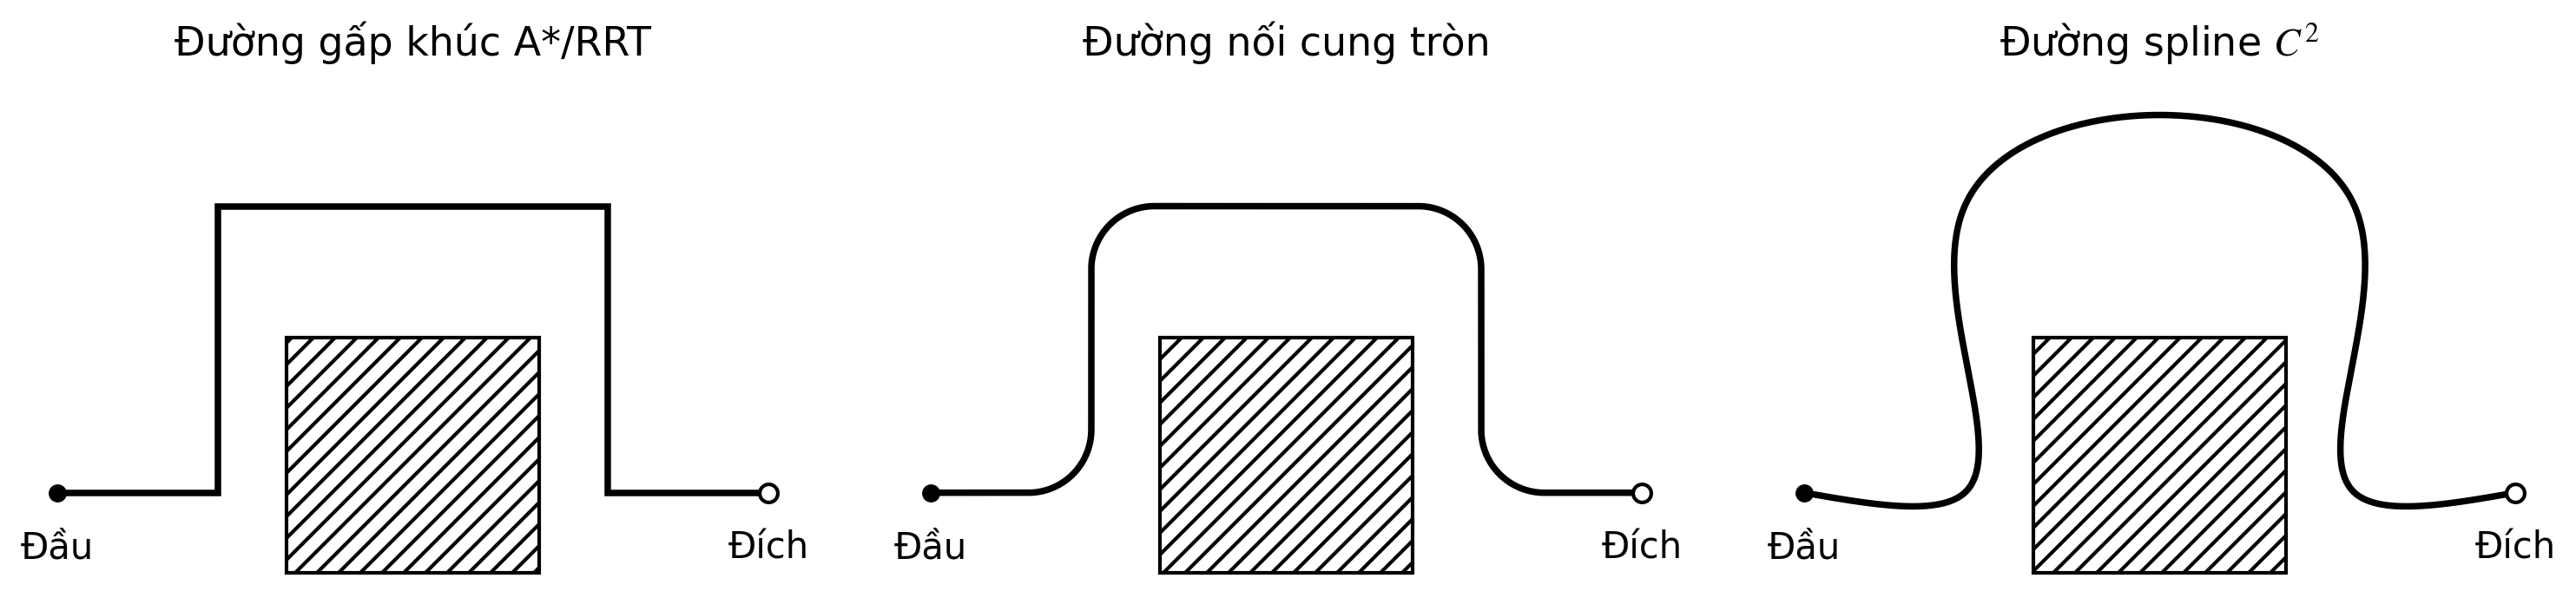
\includegraphics[width=0.8\linewidth]{so_sanh_duong_di_tranh_vat_can.png}
    \chuthichhinh[fig:so-sanh-duong-di]{So sánh đường đi gấp khúc và đường đi được làm mượt}
  \end{minipage}
\end{center}

\subsubsection*{c. Yêu cầu của bước làm mượt}

Đường mới phải giữ điểm đầu, điểm đích, hướng yêu cầu và các điểm tác vụ bắt buộc; đồng thời bảo đảm khoảng hở, hạn chế độ cong và tránh vòng lặp. Có thể bỏ các nút dư bằng nối tắt nếu toàn bộ đoạn nối an toàn. Sau làm mượt phải kiểm tra lại va chạm theo kích thước thân xe. Nếu không có đoạn chuyển tiếp phù hợp, cần đổi tuyến hoặc dùng thao tác dừng--xoay có kiểm tra.

\newpage
\subsection{Khai triển toán học đường cong tham số: Thuật toán Bézier Curve và B-Spline Curve bậc cao.}

\subsubsection*{a. Đường cong Bézier và đa thức Bernstein}

Đường Bézier được xác định từ các điểm điều khiển, thuận tiện để thiết kế đoạn bo góc và điều chỉnh hướng đầu cuối. Với \(n+1\) điểm \(\mathbf P_0,\ldots,\mathbf P_n\), biểu thức tổng quát là
\begin{equation}
  \mathbf p(u)=\sum_{i=0}^{n}\binom ni u^i(1-u)^{n-i}\mathbf P_i,
  \qquad 0\leq u\leq1.
  \label{eq:smooth-bezier}
\end{equation}
Các trọng số Bernstein không âm và có tổng bằng một, nên đường nằm trong bao lồi của các điểm điều khiển. Đường đi qua hai điểm đầu cuối nhưng thường không đi qua các điểm điều khiển ở giữa \cite{shene-bezier-notes}.

Hướng tiếp tuyến đầu phụ thuộc đoạn \(\mathbf P_0\mathbf P_1\), hướng cuối phụ thuộc đoạn \(\mathbf P_{n-1}\mathbf P_n\). Dịch các điểm lân cận đầu cuối cho phép chỉnh cách đường cong đi vào và đi ra khỏi góc cua. Thuật toán de Casteljau tính điểm trên đường bằng nội suy tuyến tính lặp, đồng thời có thể chia đường thành các đoạn nhỏ để kiểm tra hình học \cite{patrikalakis-geometric-continuity}.

\subsubsection*{b. Bézier bậc 5 và ghép các đoạn chuyển tiếp}

Bézier bậc 5 có sáu điểm điều khiển, cho phép đặt vị trí cùng đạo hàm bậc nhất và bậc hai ở cả hai đầu. Các quan hệ tại đầu đoạn có dạng
\begin{equation}
  \mathbf p'(0)=5(\mathbf P_1-\mathbf P_0),\qquad
  \mathbf p''(0)=20(\mathbf P_2-2\mathbf P_1+\mathbf P_0).
  \label{eq:smooth-bezier-endpoints}
\end{equation}
Đầu cuối có quan hệ tương tự theo thứ tự các điểm điều khiển. Nhờ đó, có thể đặt hướng tiếp tuyến theo hai đoạn cần nối và chọn đạo hàm bậc hai để điều chỉnh độ cong. Các đạo hàm này được lấy theo tham số hình học, chưa phải vận tốc và gia tốc thực của xe.

Khi ghép hai đoạn, liên tục \(C^0\) yêu cầu chung vị trí; \(C^1\) yêu cầu khớp thêm đạo hàm bậc nhất; \(C^2\) yêu cầu khớp cả đạo hàm bậc hai theo cùng tham số. Nếu hai đoạn dùng các khoảng tham số khác nhau, phải quy đổi tỷ lệ đạo hàm trước khi so khớp. Đặt các điểm điều khiển thẳng hàng chỉ giúp liên tục hướng, chưa đủ kết luận \(C^2\).

Đối với bo góc giữa hai đoạn thẳng, có thể chọn độ cong đầu cuối bằng không để chuyển tiếp êm về hình học. Tuy vậy, bậc cao không tự bảo đảm bán kính cua đủ lớn hoặc tránh được vật cản; các điểm điều khiển vẫn phải được lựa chọn trong miền an toàn.

\newpage
\subsubsection*{c. Đường B-Spline và công thức truy hồi Cox--de Boor}

B-Spline phù hợp với đường dài gồm nhiều đoạn vì bậc đường cong được chọn độc lập với số điểm điều khiển. Đường được biểu diễn bằng tổng có trọng số \(\mathbf p(u)=\sum_i N_{i,p}(u)\mathbf P_i\), trong đó \(p\) là bậc, còn \(N_{i,p}\) là hàm cơ sở xác định trên vector nút không giảm. Công thức Cox--de Boor xây dựng hàm cơ sở bậc cao từ bậc thấp:
\begin{equation}
  N_{i,p}(u)=\frac{u-u_i}{u_{i+p}-u_i}N_{i,p-1}(u)
  +\frac{u_{i+p+1}-u}{u_{i+p+1}-u_{i+1}}N_{i+1,p-1}(u).
  \label{eq:smooth-bspline}
\end{equation}
Hàm cơ sở bậc không bằng một trên khoảng nút tương ứng và bằng không ở ngoài; hạng có mẫu số bằng không được quy ước đóng góp không. Với đường kẹp hai đầu, nút đầu và cuối lặp \(p+1\) lần để đường đi qua hai điểm điều khiển biên \cite{shene-bspline-notes}.

Tại nút trong có bội \(k\leq p\), mức liên tục được bảo đảm là \(C^{p-k}\). Vì vậy, B-Spline bậc 3 với nút đơn đạt \(C^2\), còn bậc 5 với nút đơn đạt \(C^4\). Tăng bội nút làm giảm mức liên tục. Tính cục bộ giúp việc chỉnh một điểm điều khiển chỉ ảnh hưởng một vùng của đường, thuận tiện hơn khi sửa tuyến dài.

\subsubsection*{d. Lựa chọn điểm điều khiển và bảo toàn miền tự do}

Bézier thích hợp với đoạn chuyển tiếp ngắn; B-Spline phù hợp khi cần chỉnh sửa cục bộ trên nhiều đoạn. Không nên mặc nhiên coi chuỗi nút tìm đường là các điểm mà đường cong chắc chắn đi qua. Các vị trí tác vụ bắt buộc cần được đặt thành ràng buộc riêng.

Nếu các điểm điều khiển có ảnh hưởng nằm trong cùng một hành lang lồi an toàn, tính bao lồi giúp giữ đoạn cong trong hành lang đó. Chỉ kiểm tra từng điểm điều khiển ở ngoài vật cản là chưa đủ, vì đường nối giữa chúng vẫn có thể cắt vật cản. Hành lang cần tính đến kích thước xe và khoảng dự phòng; nếu không có chứng nhận bao lồi, phải kiểm tra đường cong bằng chia nhỏ hoặc kiểm tra va chạm thích hợp.

\begin{center}
  \begin{minipage}{\linewidth}
    \centering
    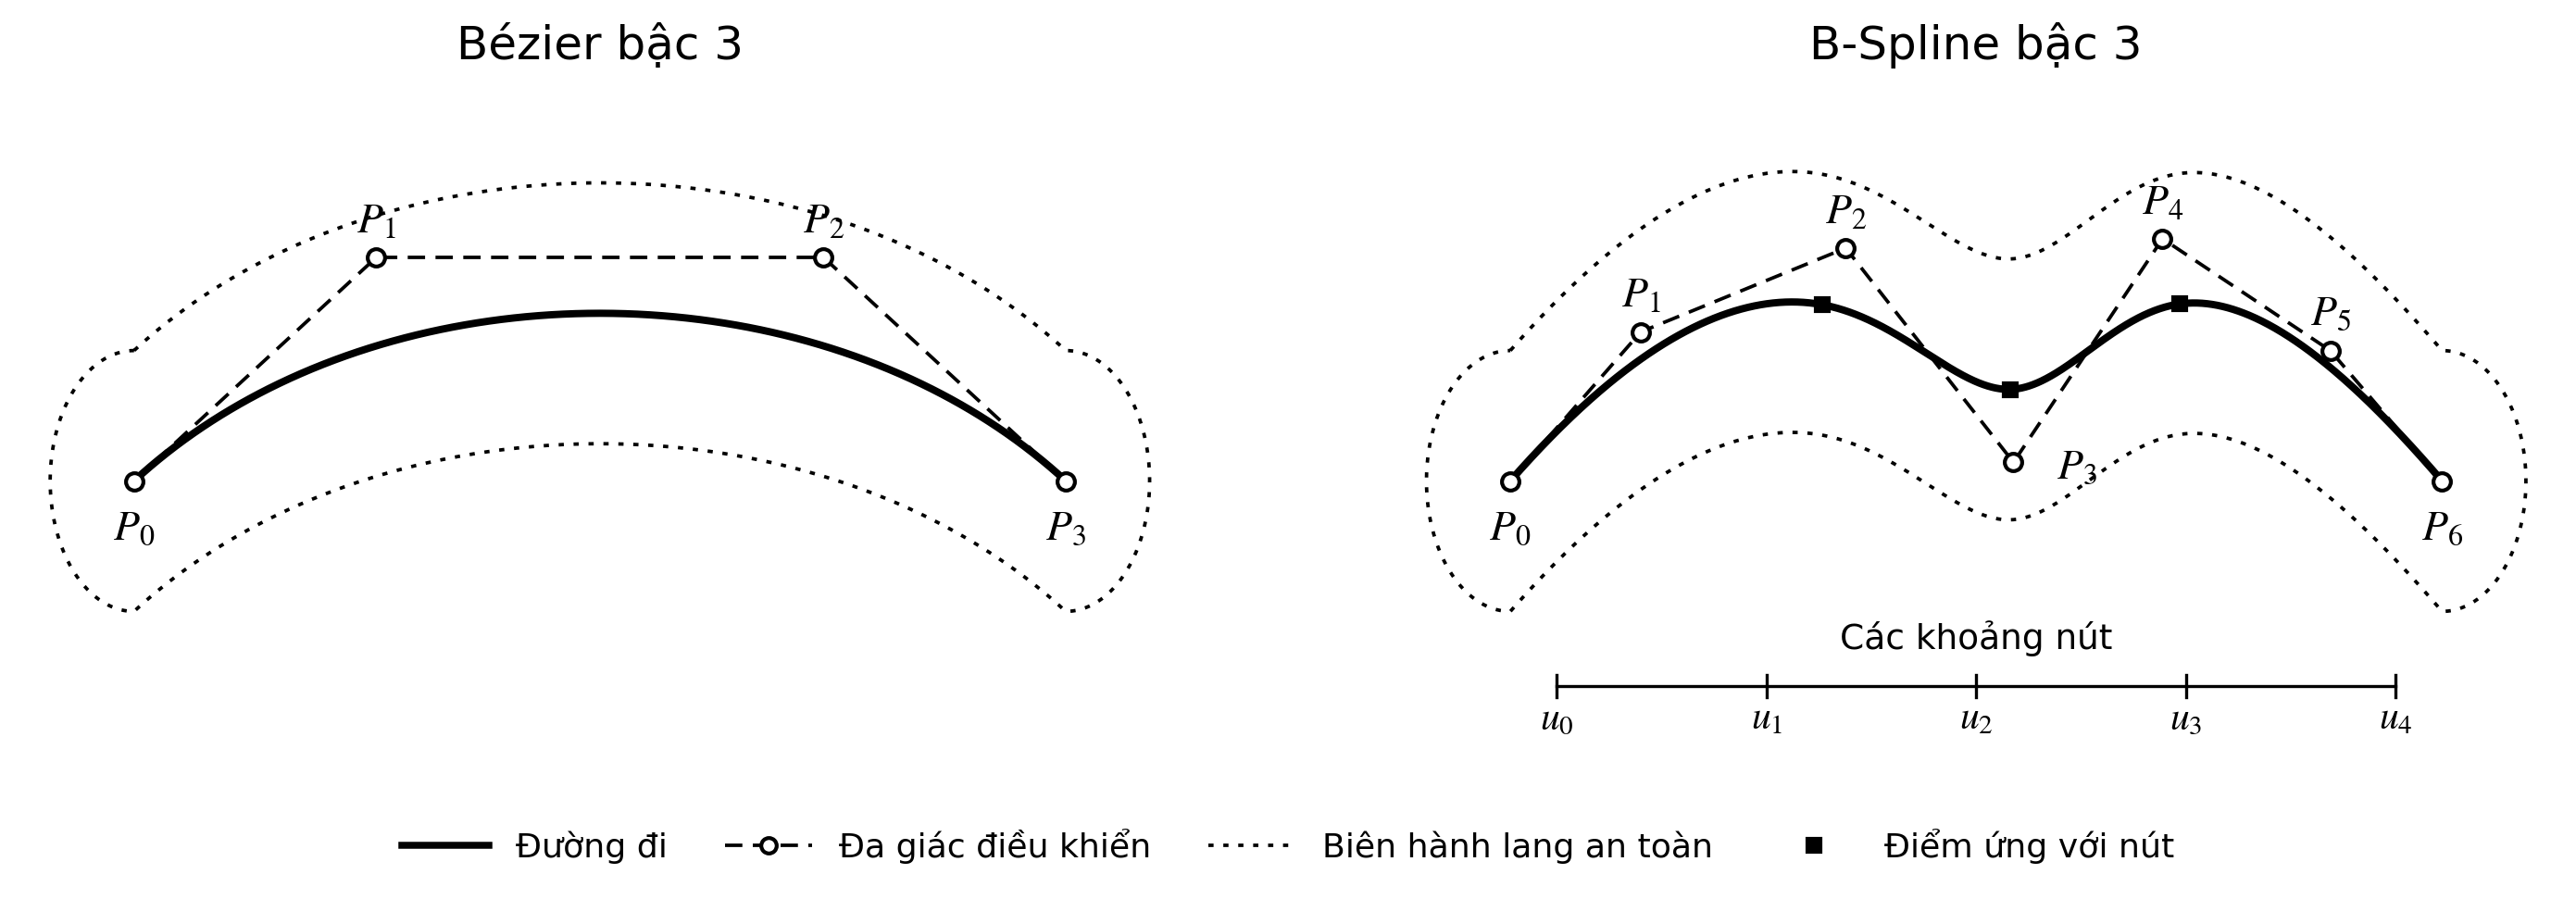
\includegraphics[width=0.8\linewidth]{bezier_bspline_hanh_lang_an_toan.png}
    \chuthichhinh[fig:bezier-bspline-hanh-lang]{Đường Bézier, B-Spline và hành lang an toàn}
  \end{minipage}
\end{center}

\newpage
\subsection{\texorpdfstring{Đảm bảo tính liên tục độ cong (\(G^{2}/C^{2}\)) tương thích với ràng buộc động học của robot 3 bánh.}{Đảm bảo tính liên tục độ cong (G2/C2) tương thích với ràng buộc động học của robot 3 bánh.}}

\subsubsection*{a. Phân biệt liên tục tham số và liên tục hình học}

Liên tục tham số \(C^2\) đòi hỏi vị trí và hai đạo hàm đầu khớp nhau theo cùng tham số. Liên tục hình học \(G^2\) yêu cầu chung vị trí, hướng tiếp tuyến và độ cong, nhưng cho phép thay đổi tốc độ chạy tham số giữa hai đoạn. Với đường chính quy, \(C^2\) kéo theo \(G^2\), còn chiều ngược lại không nhất thiết đúng nếu giữ nguyên cách tham số hóa \cite{patrikalakis-geometric-continuity}.

Phân biệt này giúp tránh nhầm độ trơn của hình dạng với độ trơn của chuyển động. Hai đoạn nối êm về hình học vẫn có thể tạo bước nhảy vận tốc nếu gán thời gian không phù hợp. Ngược lại, chỉ giảm tốc không biến một góc gãy thành một đoạn cong liên tục.

\subsubsection*{b. Độ cong và tính tương thích với ràng buộc phi holonomic}

Với đường phẳng chính quy, tức \(\|\mathbf p'(u)\|>0\), độ cong có dấu được tính bởi
\begin{equation}
  \kappa(u)=\frac{x'(u)y''(u)-y'(u)x''(u)}
                   {(x'(u)^2+y'(u)^2)^{3/2}}.
  \label{eq:smooth-curvature}
\end{equation}
Độ cong cho biết hướng tiếp tuyến thay đổi nhanh hay chậm theo chiều dài đường. Đường thẳng có độ cong bằng không; độ cong lớn tương ứng với cua gắt. Điều kiện chính quy loại trừ các điểm mà tiếp tuyến không xác định, có thể xuất hiện nếu bố trí điểm điều khiển không phù hợp.

Khi xe đi tiến và hướng thân trùng tiếp tuyến, quan hệ động học là
\begin{equation}
  \dot x=v\cos\theta,\qquad \dot y=v\sin\theta,\qquad
  \omega=v\kappa.
  \label{eq:smooth-unicycle}
\end{equation}
Cách dựng này đáp ứng ràng buộc không trượt ngang của mô hình vi sai \cite{lynch-park-modern-robotics}. Nếu vận tốc liên tục, độ cong liên tục giúp tránh bước nhảy của tốc độ quay. Khi độ cong tăng, cần giảm vận tốc để giữ yêu cầu quay trong khả năng của xe.

Xe ba bánh dùng hai bánh chủ động để tạo chuyển động, bánh tự lựa hỗ trợ cân bằng. Khả năng quay tại chỗ không thay thế yêu cầu làm mượt khi cần chạy liên tục. Với pha quay tại chỗ, vận tốc tịnh tiến bằng không nhưng tốc độ quay có thể khác không; pha này phải mô tả riêng. Nhiệm vụ đi lùi hoặc đổi chiều cũng cần phân chia các pha và xác định lại quan hệ giữa hướng thân với hướng đi.

\newpage
\subsubsection*{c. Ràng buộc tốc độ bánh xe, gia tốc và độ biến thiên độ cong}

Theo mô hình vi sai, tốc độ mỗi bánh phụ thuộc đồng thời vận tốc tâm xe và độ cong. Khi vào cua, bánh ngoài quay nhanh hơn bánh trong; vì vậy tốc độ tâm xe nhỏ chưa đủ bảo đảm cả hai động cơ đều nằm trong giới hạn. Cần xét thêm tốc độ quay thân xe và gia tốc ngang, vốn tăng theo bình phương vận tốc khi độ cong không đổi.

Độ cong liên tục giúp tránh bước nhảy tốc độ quay, nhưng chưa bảo đảm gia tốc bánh xe nhỏ hoặc liên tục. Gia tốc quay của thân xe phụ thuộc cả gia tốc dọc lẫn tốc độ biến thiên độ cong theo chiều dài đường. Do đó, cần kiểm tra những vùng đổi độ cong nhanh và giảm tốc trước khi tới đoạn cua. Đường bậc cao tạo thuận lợi cho chuyển tiếp, song vẫn phải kiểm tra các giới hạn cụ thể của truyền động.

\subsubsection*{d. Kết hợp với quy luật thời gian và quy trình áp dụng}

Sau khi chốt hình học, quy luật thời gian xác định robot đi qua từng vị trí lúc nào và nhanh đến mức nào. Profile chữ S có thể dùng cho chuyển động dọc đường, nhưng phải điều chỉnh theo giới hạn cục bộ tại các đoạn cong. Giới hạn jerk của chuyển động dọc đường chưa tự bảo đảm mọi thành phần gia tốc và jerk trên mặt phẳng đều phù hợp.

Quy trình áp dụng gồm tìm đường và loại nút dư; xác định điểm bắt buộc cùng hành lang an toàn; dựng Bézier hoặc B-Spline; kiểm tra tiếp tuyến, độ cong và va chạm; sau đó gán thời gian có xét tăng tốc, giảm tốc. Cuối cùng, sinh tham chiếu vị trí, hướng, vận tốc và tốc độ quay, quy đổi sang lệnh hai bánh và kiểm tra trước khi đưa tới bộ bám.

Chất lượng được đánh giá qua chiều dài đường, khoảng hở nhỏ nhất, độ cong lớn nhất, tốc độ/gia tốc bánh xe và thời gian hành trình. Đường mượt chỉ được chấp nhận khi đồng thời an toàn về hình học và phù hợp với khả năng chuyển động của robot.

\begin{center}
  \begin{minipage}{\linewidth}
    \centering
    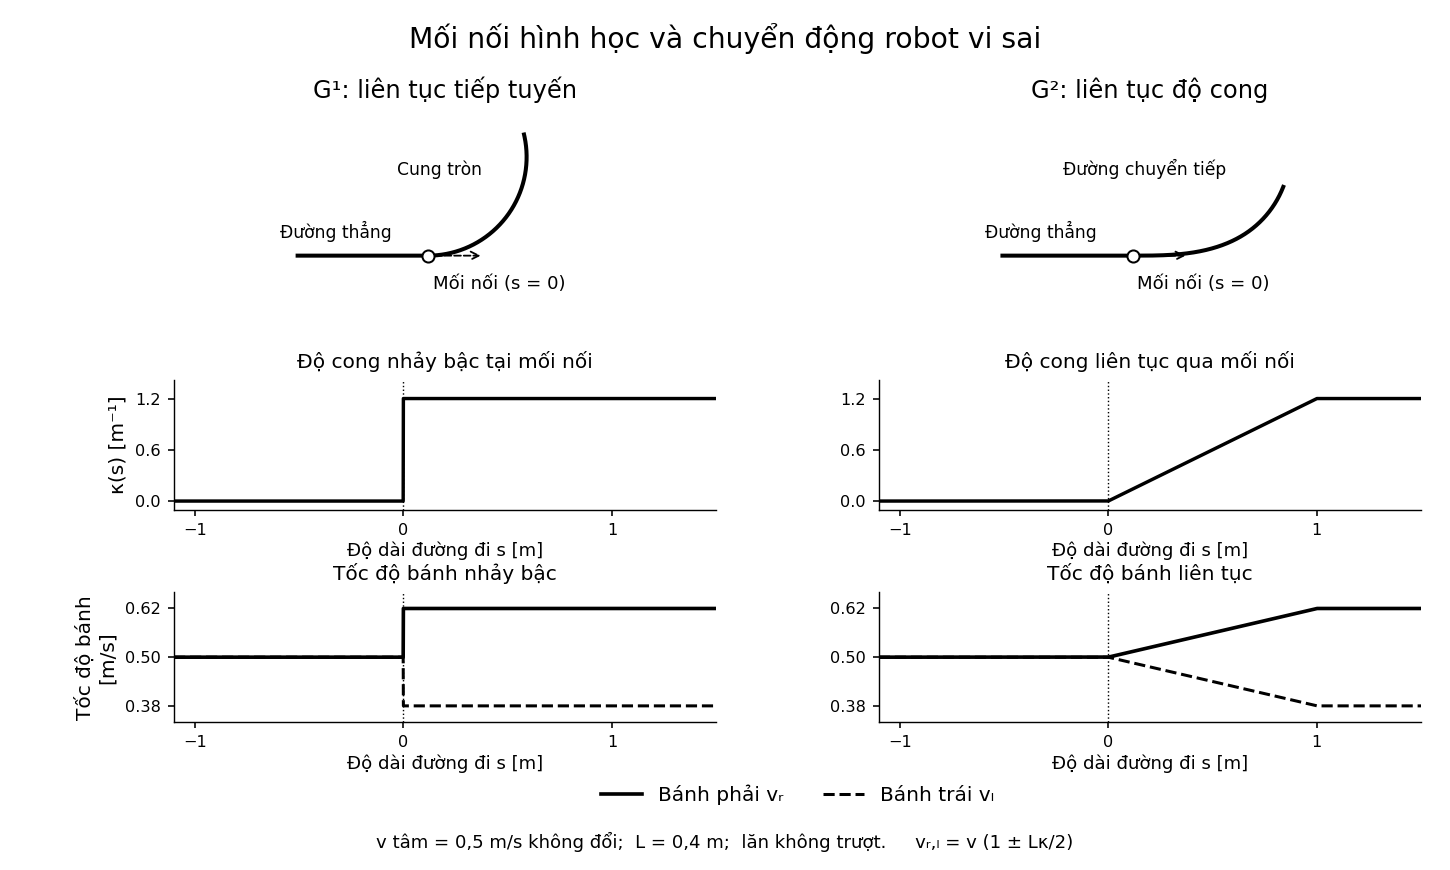
\includegraphics[width=\linewidth]{moi_noi_G1_G2_do_cong_toc_do_banh.png}
    \chuthichhinh[fig:moi-noi-g1-g2]{Mối nối liên tục hình học và ảnh hưởng đến chuyển động robot}
  \end{minipage}
\end{center}


\chapter{CÁC THUẬT TOÁN QUY HOẠCH QUỸ ĐẠO VÀ MÔ PHỎNG}

\section{Nhóm Thuật toán Tìm đường Dựa trên Đồ thị (Graph-based Planning)}

Trong nhóm phương pháp này, môi trường chuyển động được biểu diễn bằng đồ thị \(G=(\mathcal{V},\mathcal{E})\), trong đó \(\mathcal{V}\) là tập đỉnh đại diện cho các trạng thái hợp lệ và \(\mathcal{E}\) là tập cạnh đại diện cho các chuyển động được phép. Đặt \(V=|\mathcal{V}|\), \(E=|\mathcal{E}|\); mỗi cạnh \((u,v)\) có trọng số không âm \(w(u,v)\). Bài toán tìm đường từ đỉnh xuất phát \(s\) đến đỉnh đích \(t\) được viết dưới dạng
\begin{equation}
  P^{*}=\operatorname*{arg\,min}_{P:s\leadsto t} J(P),
  \qquad J(P)=\sum_{(u,v)\in P}w(u,v).
  \label{eq:graph-path-cost}
\end{equation}
Nếu trọng số là chiều dài đoạn nối, nghiệm là đường ngắn nhất trên đồ thị. Khi trọng số chứa thêm chi phí địa hình hoặc khoảng cách đến vật cản, nghiệm tối ưu được hiểu theo hàm chi phí đã chọn, không nhất thiết có chiều dài hình học nhỏ nhất.

Đối với robot di động trong mặt phẳng, một cách xây dựng đồ thị là chia bản đồ thành các ô lưới và nối những ô tự do lân cận. Trước khi tìm đường, cần tính đến kích thước robot bằng cách mở rộng vật cản theo hình học thân xe và khoảng dự phòng an toàn. Với mô hình robot tròn có bán kính \(r\), vùng cấm cho tâm robot có thể được xây dựng bằng tổng Minkowski giữa vật cản và đĩa bán kính \(r\). Khi đó, kiểm tra một điểm tâm xe có ý nghĩa đối với cả thân xe. Với robot có hình dạng phụ thuộc hướng, có thể dùng mô hình bao tròn bảo thủ hoặc đưa góc hướng vào trạng thái. Các cơ sở tìm kiếm trên đồ thị được trình bày trong \cite[Chương 2]{lavalle-planning-2006}.

\subsection{Thuật toán Dijkstra}

\subsubsection*{a. Nguyên lý mở rộng đỉnh và cập nhật chi phí}

Dijkstra giải bài toán đường đi ngắn nhất với trọng số cạnh không âm. Thuật toán duy trì \(g(v)\), là chi phí tốt nhất hiện biết từ \(s\) đến đỉnh \(v\), cùng con trỏ \(\operatorname{parent}(v)\) để truy vết đường đi. Ban đầu, \(g(s)=0\), còn \(g(v)=+\infty\) với mọi \(v\neq s\). Ở mỗi vòng lặp, đỉnh chưa chốt có chi phí nhỏ nhất được lấy ra để mở rộng. Với một đỉnh lân cận \(v\) của đỉnh đang xét \(u\), phép nới lỏng cạnh (relaxation) thực hiện theo quy tắc
\begin{equation}
  \text{nếu } g(u)+w(u,v)<g(v),\quad
  \begin{cases}
    g(v)\leftarrow g(u)+w(u,v),\\
    \operatorname{parent}(v)\leftarrow u.
  \end{cases}
  \label{eq:dijkstra-relax}
\end{equation}
Do các trọng số không âm, khi một đỉnh có nhãn nhỏ nhất được lấy ra hợp lệ, không còn đường đi qua các đỉnh chưa chốt có thể làm giảm chi phí của nó. Vì vậy, chi phí tại đỉnh này được chốt và thuật toán tiếp tục với các đỉnh còn lại \cite{lavalle-planning-2006}.

Trình tự xử lý có thể mô tả như sau:
\begin{enumerate}[label=\arabic*.]
  \item Khởi tạo các nhãn chi phí, con trỏ cha và hàng đợi; đưa \(s\) vào hàng đợi với khóa bằng \(0\).
  \item Lấy ra đỉnh \(u\) có khóa nhỏ nhất. Bỏ qua bản ghi đã lỗi thời hoặc đỉnh đã chốt nếu cách cài đặt có thể tạo bản ghi trùng.
  \item Nếu \(u=t\), kết thúc tìm kiếm. Nếu chưa đến đích, chốt \(u\), xét từng cạnh đi ra và cập nhật các đỉnh lân cận theo công thức \eqref{eq:dijkstra-relax}.
  \item Nếu hàng đợi rỗng trước khi chốt được \(t\), kết luận không có đường đi trên đồ thị đang xét. Nếu tìm thấy đích, lần ngược các con trỏ cha từ \(t\) về \(s\) rồi đảo thứ tự để thu được đường đi.
\end{enumerate}
Điều kiện dừng phải kiểm tra khi đích được lấy ra với khóa hợp lệ nhỏ nhất; việc đích mới được phát hiện chưa đủ để khẳng định đường đi tối ưu.

\subsubsection*{b. Hàng đợi ưu tiên và độ phức tạp}

Hàng đợi ưu tiên (Priority Queue) lưu các đỉnh chờ xét và cho phép lấy ra đỉnh có \(g\) nhỏ nhất. Nếu dùng heap nhị phân, thao tác lấy phần tử nhỏ nhất và giảm khóa có chi phí \(O(\log V)\). Trong thực hành, có thể đưa bản ghi mới vào heap mỗi khi tìm được chi phí tốt hơn; khi lấy ra, cần so sánh khóa lưu trong bản ghi với \(g(v)\) hiện tại để loại bỏ dữ liệu cũ. Cách này đơn giản hơn thao tác giảm khóa nhưng có thể lưu nhiều bản ghi cho một đỉnh.

Độ phức tạp phụ thuộc cấu trúc dữ liệu được sử dụng:
\begin{itemize}
  \item \textbf{Mảng nhãn và danh sách kề:} Mỗi lần chọn đỉnh nhỏ nhất phải quét tối đa \(V\) đỉnh. Có tối đa \(V\) lần chọn và tổng cộng \(E\) cạnh được xét, nên thời gian là \(O(V^{2}+E)\).
  \item \textbf{Heap nhị phân có giảm khóa và danh sách kề:} Thời gian là \(O((V+E)\log V)\), phù hợp với đồ thị thưa như lưới có số láng giềng bị chặn.
  \item \textbf{Heap Fibonacci:} Giới hạn lý thuyết là \(O(E+V\log V)\), nhưng cấu trúc phức tạp hơn và không nhất thiết đem lại lợi ích trong một cài đặt quy mô nhỏ \cite{lavalle-planning-2006}.
\end{itemize}
Với heap có giảm khóa, tổng bộ nhớ cho đồ thị và dữ liệu tìm kiếm là \(O(V+E)\). Cách đưa bản ghi trùng vào heap có thể cần tới \(O(E)\) bản ghi trong một đồ thị đơn. Như vậy, \(O(V^{2}+E)\) là giới hạn của cách chọn đỉnh bằng mảng, không phải giới hạn áp dụng cho mọi cài đặt sử dụng hàng đợi ưu tiên.

\begin{center}
  \begin{minipage}{\linewidth}
    \centering
    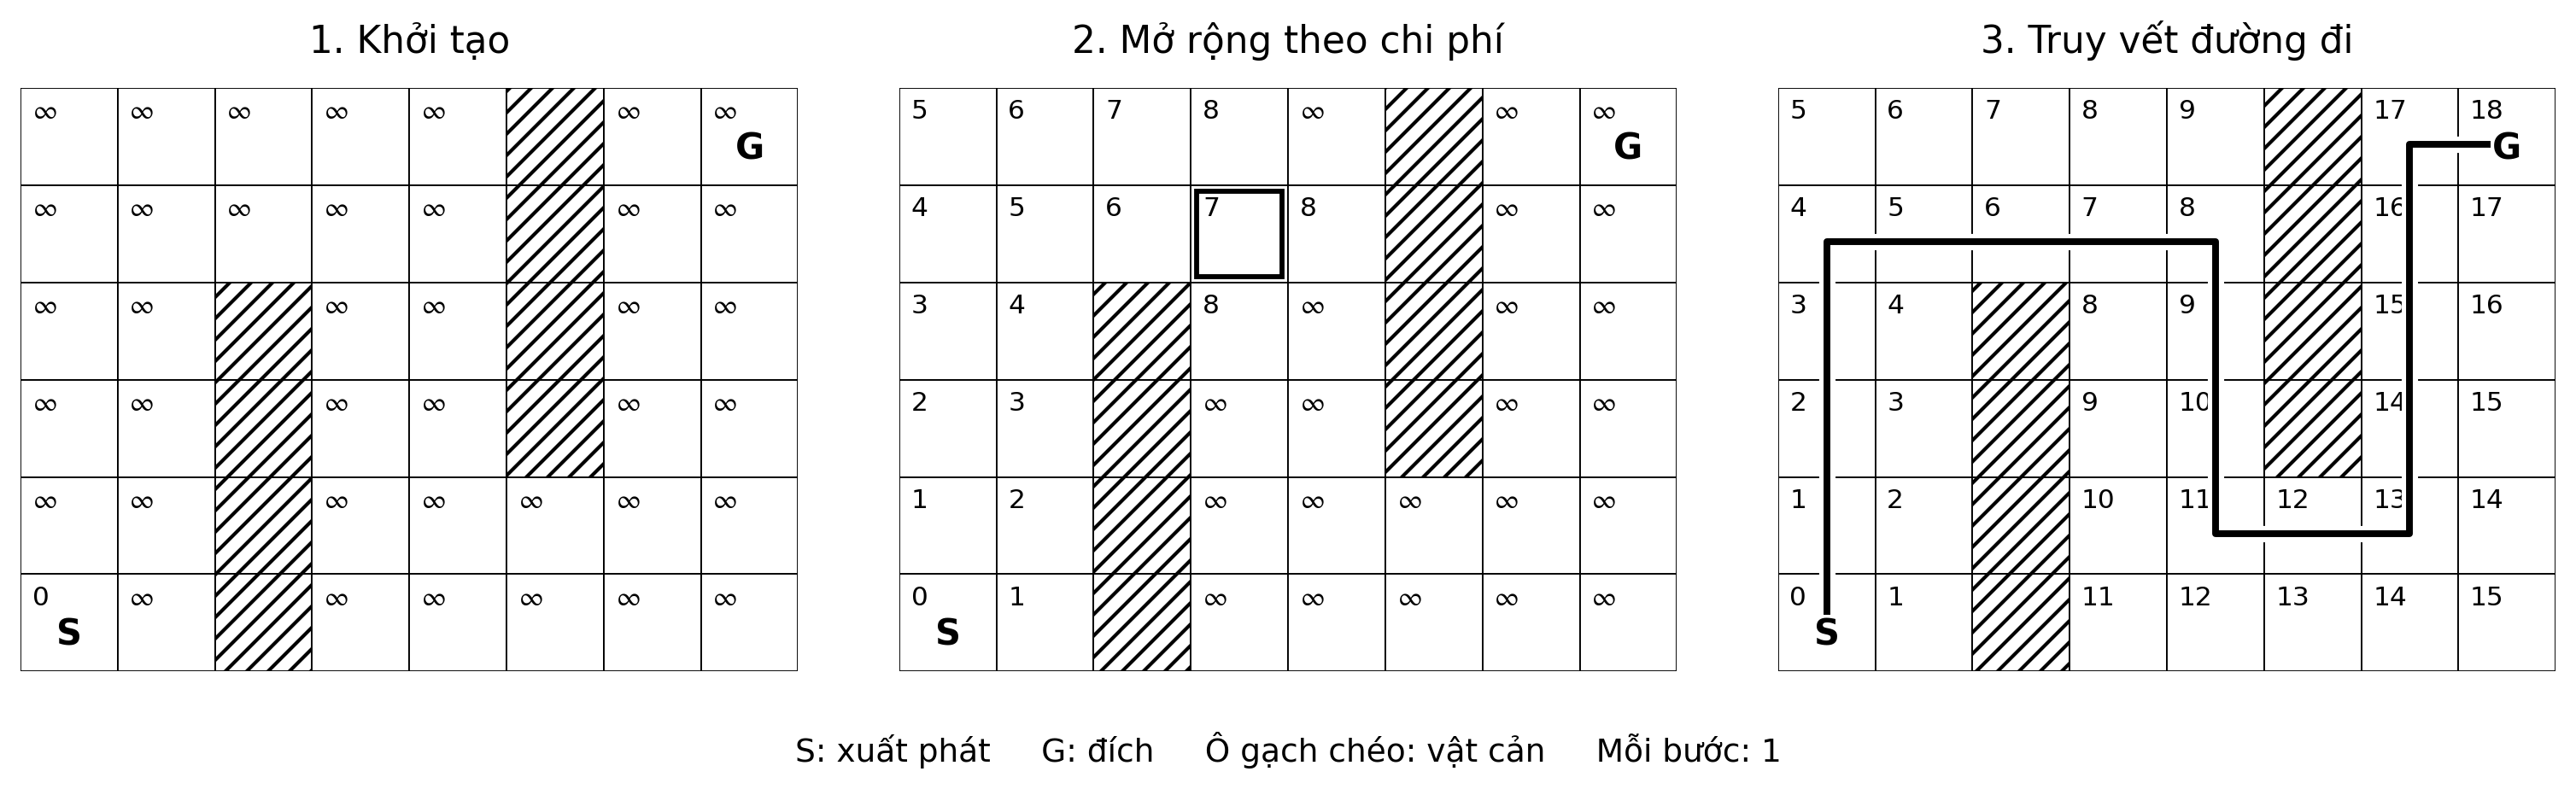
\includegraphics[width=\linewidth]{dijkstra_mo_rong_tren_luoi.png}
    \chuthichhinh[fig:dijkstra-mo-rong]{Các bước mở rộng đỉnh của Dijkstra trên bản đồ lưới}
  \end{minipage}
\end{center}

\subsubsection*{c. Vai trò đối với bài toán của đề tài}

Dijkstra cung cấp một nghiệm đối chứng để kiểm tra chi phí đường đi của các thuật toán tìm kiếm khác trên cùng đồ thị. Hạn chế là thuật toán không sử dụng thông tin về hướng của đích, nên có thể mở rộng nhiều đỉnh ở những vùng không cần thiết. Ngoài ra, tối ưu trên lưới không đồng nghĩa với tối ưu trong không gian liên tục. Kết quả thường là một đường gấp khúc, cần được làm mượt, kiểm tra va chạm lại và gán quy luật vận tốc trước khi chuyển thành quỹ đạo cho robot.

\subsection{Thuật toán A*}

\subsubsection*{a. Hàm đánh giá và điều kiện của heuristic}

A* bổ sung một ước lượng chi phí còn lại đến đích để định hướng việc mở rộng đỉnh. Thay vì chỉ sắp xếp theo \(g(n)\), thuật toán chọn đỉnh có giá trị nhỏ nhất của
\begin{equation}
  f(n)=g(n)+h(n),
  \label{eq:astar-score}
\end{equation}
trong đó \(g(n)\) là chi phí tốt nhất hiện biết từ điểm xuất phát đến \(n\), còn \(h(n)\) là heuristic ước lượng chi phí từ \(n\) đến đích. Khi \(h(n)=0\) với mọi đỉnh, A* trở thành Dijkstra \cite{lavalle-planning-2006}.

Để duy trì tính tối ưu, heuristic phải phù hợp với trọng số cạnh và mô hình chuyển động. Gọi \(h^{*}(n)\) là chi phí tối ưu thực sự từ \(n\) đến đích. Một heuristic chấp nhận được (admissible) thỏa mãn
\begin{equation}
  0\leq h(n)\leq h^{*}(n),\qquad h(t)=0.
\end{equation}
Heuristic nhất quán (consistent) còn thỏa mãn \(h(u)\leq w(u,v)+h(v)\) với mọi cạnh \((u,v)\). Với heuristic nhất quán, một đỉnh đã đóng không cần mở lại. Nếu heuristic chỉ chấp nhận được nhưng không nhất quán, cài đặt tìm kiếm trên đồ thị phải cho phép mở lại đỉnh khi phát hiện chi phí \(g\) tốt hơn. Việc dùng heuristic lớn hơn chi phí thực có thể tăng mức độ hướng đích nhưng không còn bảo đảm nghiệm tối ưu.

\subsubsection*{b. Heuristic Euclidean, Manhattan và Diagonal}

Xét các tọa độ ô lưới \((i,j)\) và tọa độ đích \((i_t,j_t)\); đặt \(\Delta_i=|i-i_t|\), \(\Delta_j=|j-j_t|\). Gọi \(D>0\) là chi phí một bước ngang hoặc dọc. Nếu tối ưu chiều dài, \(D\) có thể bằng kích thước cạnh ô lưới.
\begin{itemize}
  \item \textbf{Euclidean:} Ước lượng theo đoạn thẳng nối tới đích,
  \[
    h_E(n)=D\sqrt{\Delta_i^{2}+\Delta_j^{2}}.
  \]
  Đây là cận dưới thích hợp khi chi phí của các cạnh không nhỏ hơn chiều dài Euclidean tương ứng theo cùng tỷ lệ. Trên lưới, đường thực tế có thể dài hơn do vật cản và giới hạn hướng di chuyển.
  \item \textbf{Manhattan:} Phù hợp với lưới bốn hướng có chi phí \(D\) cho mỗi bước ngang hoặc dọc,
  \[
    h_M(n)=D(\Delta_i+\Delta_j).
  \]
  Nếu cho phép bước chéo với giá \(\sqrt{2}D\), Manhattan có thể đánh giá quá cao chi phí còn lại và làm mất điều kiện chấp nhận được.
  \item \textbf{Diagonal:} Với lưới tám hướng, chi phí bước chéo \(D_2\) và \(D\leq D_2\leq 2D\), khoảng cách khi bỏ qua vật cản là
  \begin{equation}
    h_D(n)=D\max(\Delta_i,\Delta_j)
      +(D_2-D)\min(\Delta_i,\Delta_j).
    \label{eq:diagonal-heuristic}
  \end{equation}
  Khi \(D_2=\sqrt{2}D\), công thức là khoảng cách octile; khi \(D_2=D\), công thức trở thành khoảng cách Chebyshev. Hai trường hợp tương ứng hai mô hình chi phí khác nhau.
\end{itemize}
Chẳng hạn, với \(\Delta_i=3\), \(\Delta_j=2\) và \(D=1\), ta có \(h_E=\sqrt{13}\), \(h_M=5\), còn octile bằng \(1+2\sqrt{2}\). Với lưới tám hướng và chi phí chéo \(\sqrt{2}\), đường không vật cản chỉ cần hai bước chéo và một bước ngang; do đó giá trị Manhattan bằng \(5\) là quá lớn. Ví dụ này cho thấy việc chọn heuristic phải xuất phát từ những bước di chuyển thực sự được phép.

Nếu trọng số chứa chi phí địa hình, có thể xây dựng heuristic từ mức chi phí tối thiểu cho một đơn vị khoảng cách; các khoản phạt không âm có thể được bỏ qua khi lập cận dưới. Nếu mục tiêu là thời gian, heuristic cũng phải có đơn vị thời gian, chẳng hạn khoảng cách chia cho một cận trên hợp lệ của tốc độ.

\subsubsection*{c. Tập mở, tập đóng và trình tự tìm kiếm}

Tập mở (Open Set) chứa các đỉnh đã phát hiện và còn chờ mở rộng, thường được quản lý bằng hàng đợi ưu tiên theo \(f\). Tập đóng (Closed Set) ghi các đỉnh đã mở rộng. Quy trình xử lý gồm khởi tạo \(s\), lấy đỉnh có \(f\) nhỏ nhất, kiểm tra điều kiện đích, nới lỏng các cạnh và cập nhật con trỏ cha. Nếu tìm thấy đường tốt hơn tới một đỉnh trong tập mở, khóa ưu tiên phải được cập nhật hoặc phải thêm bản ghi mới có cơ chế bỏ qua bản ghi lỗi thời. Việc xử lý đỉnh đã đóng tuân theo điều kiện nhất quán đã nêu ở trên.

A* dừng khi đỉnh đích được lấy ra hợp lệ khỏi tập mở. Sau đó, đường đi được truy vết bằng các con trỏ cha. Trong bản đồ lưới có bước chéo, cần kiểm tra đoạn nối giữa hai ô và loại các chuyển động cắt qua góc vật cản; việc chỉ kiểm tra hai ô đầu cuối không bảo đảm an toàn cho đoạn đi qua giữa chúng.

\noindent\begin{minipage}{\linewidth}
  \begin{center}
    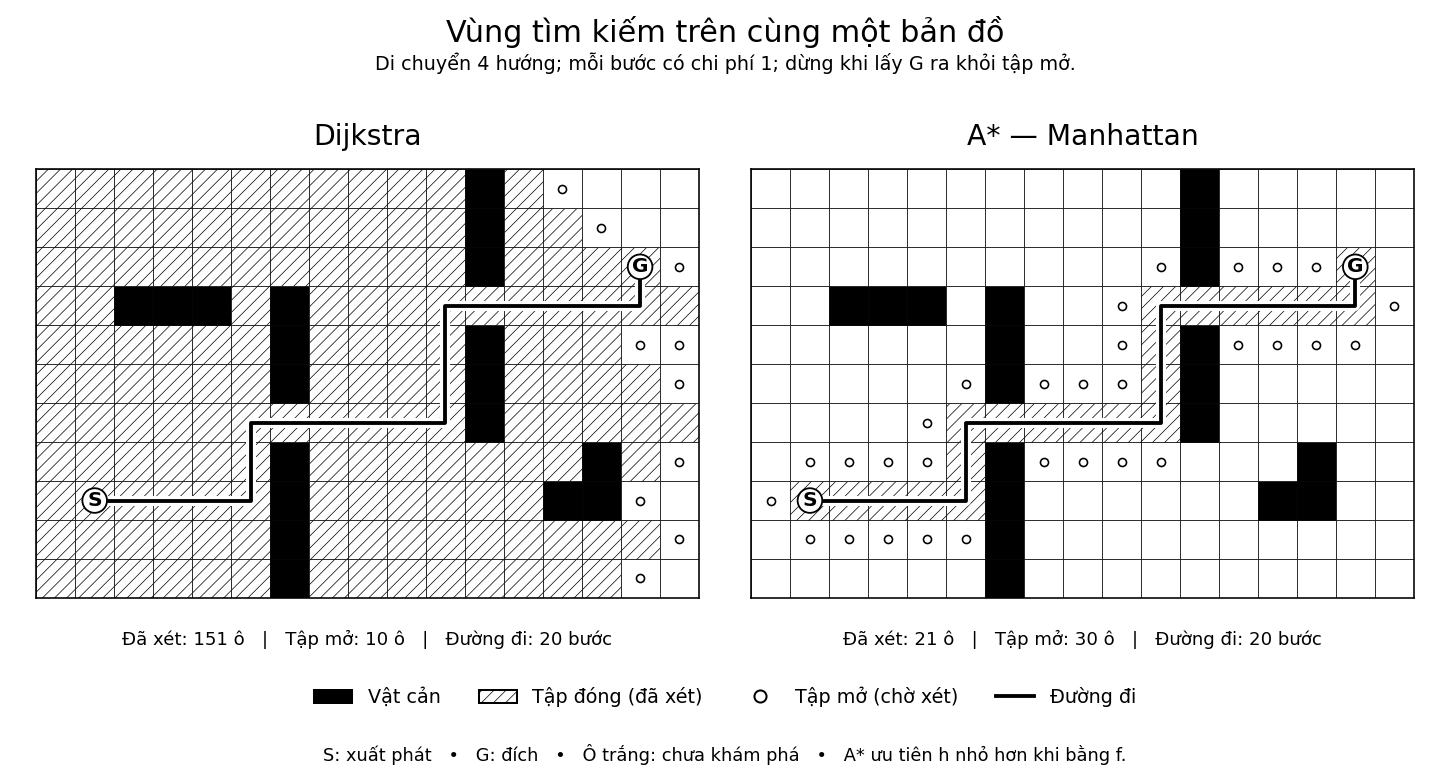
\includegraphics[width=\linewidth]{so_sanh_dijkstra_astar_tap_mo_tap_dong.png}
    \chuthichhinh[fig:dijkstra-astar-tap-mo-dong]{So sánh vùng tìm kiếm của Dijkstra và A*}
  \end{center}
\end{minipage}\par\medskip

Với heuristic hữu ích, A* thường giảm số đỉnh phải mở rộng so với Dijkstra, nhưng không có bảo đảm mức giảm cố định trên mọi bản đồ. Trong trường hợp xấu, thuật toán vẫn có thể xét phần lớn đồ thị. Với heuristic nhất quán và heap nhị phân có giảm khóa, thời gian tìm kiếm trên đồ thị hữu hạn được chặn bởi \(O((V+E)\log V)\). Kết quả của A* vẫn cần qua bước làm mượt và tạo profile vận tốc; nếu sử dụng trạng thái chỉ gồm \((x,y)\), các ràng buộc hướng và động học của xe chưa tự động được bảo đảm.

\section{Nhóm Thuật toán Lấy mẫu Ngẫu nhiên (Sampling-based Planning)}

Các phương pháp lấy mẫu xây dựng biểu diễn hữu hạn của không gian cấu hình bằng những trạng thái được chọn theo một quy tắc lấy mẫu. Gọi \(\mathcal{C}_{\mathrm{free}}\) là miền cấu hình không va chạm, \(q_s\) và \(q_g\) là cấu hình đầu và đích. Mỗi mẫu phải được kiểm tra tính hợp lệ; mỗi cạnh nối giữa hai mẫu phải được kiểm tra trên toàn bộ chuyển động do bộ lập kế hoạch cục bộ tạo ra. Vì vậy, việc hai đầu mút nằm trong miền tự do không đủ để kết luận cạnh nối an toàn.

Trong mô phỏng hình học cho robot di động, có thể bắt đầu từ \(q=(x,y)\) trên bản đồ đã mở rộng vật cản. Đối với bài toán xét cả hướng thân xe, trạng thái có thể là \(q=(x,y,\theta)\). Khoảng cách giữa hai trạng thái khi đó phải xử lý tính tuần hoàn của góc và cân đối đơn vị giữa vị trí và hướng. Nếu cần thỏa mãn ràng buộc phi holonomic, bộ nối cục bộ phải sinh chuyển động khả thi thay vì tùy ý nội suy thẳng trong không gian trạng thái.

\subsection{Thuật toán PRM (Probabilistic Roadmaps)}

\subsubsection*{a. Giai đoạn học và xây dựng mạng lưới}

PRM xây dựng một mạng đường đi có thể tái sử dụng cho nhiều cặp xuất phát--đích trong cùng môi trường tĩnh. Theo phương pháp gốc, thuật toán gồm giai đoạn học và giai đoạn truy vấn \cite{kavraki-prm-1996}. Trong giai đoạn học, các cấu hình hợp lệ được lưu thành tập đỉnh \(\mathcal{V}_R\), còn các chuyển động nối hợp lệ được lưu thành tập cạnh \(\mathcal{E}_R\), tạo thành roadmap \(G_R=(\mathcal{V}_R,\mathcal{E}_R)\).

Quá trình xây dựng roadmap gồm:
\begin{enumerate}[label=\arabic*.]
  \item Lấy mẫu \(q\) trong miền cấu hình. Loại các mẫu va chạm hoặc vi phạm giới hạn của robot; giữ lại mẫu trong \(\mathcal{C}_{\mathrm{free}}\).
  \item Tìm các mẫu lân cận theo bán kính kết nối hoặc theo số láng giềng được chọn. Quy tắc này ảnh hưởng đến mức liên thông và chi phí xây dựng mạng.
  \item Với từng cặp ứng viên, gọi bộ lập kế hoạch cục bộ. Trong mô hình điểm hình học, đường nối có thể là
  \[
    q(\lambda)=(1-\lambda)q_i+\lambda q_j,
    \qquad 0\leq\lambda\leq1.
  \]
  Chỉ thêm cạnh nếu toàn bộ đường nối không va chạm. Với robot có ràng buộc động học, thay đoạn thẳng bằng chuyển động phù hợp với mô hình xe.
  \item Gán trọng số cho cạnh, chẳng hạn chiều dài đường nối, và tiếp tục bổ sung mẫu đến khi đạt giới hạn số mẫu hoặc ngân sách tính toán.
\end{enumerate}
Trong mô hình hình học đối xứng, roadmap thường là đồ thị vô hướng. Nếu một chuyển động hợp lệ theo chiều đi nhưng không hợp lệ theo chiều ngược lại, phải biểu diễn bằng cạnh có hướng. Khi kiểm tra va chạm bằng các điểm rời rạc trên cạnh, bước kiểm tra phải đủ nhỏ theo độ phân giải bản đồ và kích thước vật cản, hoặc sử dụng phép kiểm tra liên tục; lấy mẫu quá thưa có thể bỏ sót một vật cản nằm giữa hai điểm kiểm tra.

\subsubsection*{b. Giai đoạn truy vấn đường đi}

Khi nhận \(q_s\) và \(q_g\), thuật toán kiểm tra hai cấu hình, thêm chúng vào roadmap và thử kết nối với các đỉnh lân cận bằng cùng bộ lập kế hoạch cục bộ. Sau đó, Dijkstra hoặc A* được dùng để tìm đường trong mạng. Nếu tìm thấy, chuỗi cạnh được ghép thành đường đi từ đầu đến đích. Nếu không tìm thấy, có thể tăng số mẫu hoặc mở rộng tập kết nối rồi truy vấn lại; một lần truy vấn thất bại trên roadmap hữu hạn chưa chứng minh môi trường không có đường đi.

\noindent\begin{minipage}{\linewidth}
  \begin{center}
    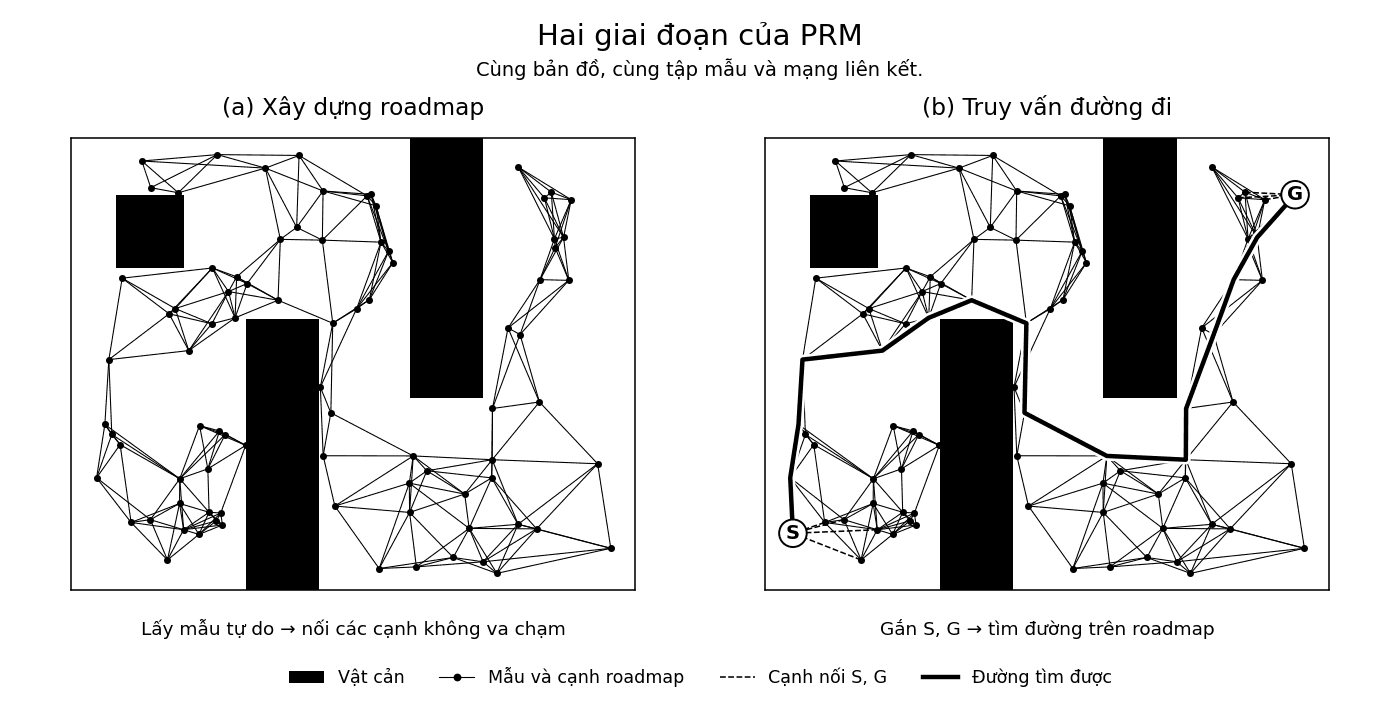
\includegraphics[width=\linewidth]{prm_xay_dung_va_truy_van.png}
    \chuthichhinh[fig:prm-xay-dung-truy-van]{Hai giai đoạn xây dựng và truy vấn mạng PRM}
  \end{center}
\end{minipage}\par\medskip

Giai đoạn học chỉ xây dựng mạng lưới, không phải huấn luyện một mô hình học máy. Lợi ích của PRM xuất hiện rõ khi chi phí xây dựng mạng được phân bổ cho nhiều truy vấn trong bản đồ ít thay đổi. Khi vật cản thay đổi, những cạnh và đỉnh bị ảnh hưởng phải được kiểm tra lại trước khi tiếp tục sử dụng.

\subsubsection*{c. Đặc điểm và giới hạn}

Khó khăn của lấy mẫu đều là các hành lang hẹp chiếm một phần nhỏ thể tích không gian tự do, nên ít mẫu rơi vào vùng cần thiết. Tăng mật độ mẫu hoặc lấy mẫu có thiên hướng gần vùng khó có thể cải thiện khả năng kết nối, nhưng cũng làm tăng số lần kiểm tra va chạm. Số láng giềng quá nhỏ có thể làm mạng rời rạc, còn kết nối quá nhiều làm tăng chi phí xây dựng.

Tính đầy đủ xác suất có nghĩa là xác suất tìm được đường tiến tới \(1\) khi số mẫu tăng, nếu bài toán có đường khả thi với khoảng hở phù hợp và các giả thiết về lấy mẫu, kết nối được thỏa mãn. Đây không phải bảo đảm thành công với một số mẫu hữu hạn. PRM thông thường cũng không tự động có tính tối ưu tiệm cận; muốn khẳng định tính chất này phải dùng biến thể và quy tắc kết nối tương ứng, chẳng hạn PRM* \cite{karaman-frazzoli-2011}. Trong đề tài, PRM thích hợp để đánh giá khả năng tái sử dụng mạng đường đi trong môi trường tĩnh và ảnh hưởng của số mẫu đối với tỷ lệ thành công.

\subsection{\texorpdfstring{Thuật toán RRT và RRT*}{Thuật toán RRT và RRT*}}

\subsubsection*{a. Cơ chế phát triển cây RRT}

RRT (Rapidly-exploring Random Tree) phát triển một cây tìm kiếm có gốc tại \(q_s\). Khác với PRM xây dựng một mạng dùng cho nhiều truy vấn, RRT cơ bản mở rộng cây để giải một truy vấn cụ thể. Tại mỗi vòng lặp, thuật toán lấy một cấu hình ngẫu nhiên \(q_{\mathrm{rand}}\), tìm đỉnh gần nhất \(q_{\mathrm{near}}\) trong cây rồi thử tiến một đoạn về phía mẫu. Cơ chế này tạo thiên hướng khám phá các vùng chưa được cây bao phủ \cite{lavalle-rrt-1998}.

Trong mô hình hình học Euclidean, phép mở rộng có độ dài tối đa \(\eta>0\) được viết là
\begin{equation}
  q_{\mathrm{new}}=q_{\mathrm{near}}
    +\min\!\left(1,\frac{\eta}{\|q_{\mathrm{rand}}-q_{\mathrm{near}}\|}\right)
      (q_{\mathrm{rand}}-q_{\mathrm{near}}).
  \label{eq:rrt-steer}
\end{equation}
Mẫu trùng với đỉnh gần nhất được bỏ qua để tránh phép chia cho \(0\). Nếu chuyển động từ \(q_{\mathrm{near}}\) đến \(q_{\mathrm{new}}\) hợp lệ, đỉnh mới được thêm vào cây và nhận \(q_{\mathrm{near}}\) làm cha; nếu không, lần mở rộng bị loại.

Thuật toán lặp đến khi một đỉnh có thể nối hợp lệ tới đích hoặc đạt ngân sách tính toán. Trong không gian liên tục, xác suất lấy đúng một điểm đích riêng lẻ thường bằng \(0\), nên có thể dùng một vùng đích có dung sai hoặc chủ động thử nối tới \(q_g\). Nếu dùng vùng đích, phải báo cáo dung sai và không coi điểm trong vùng là chính xác bằng \(q_g\). Một tỷ lệ lấy mẫu hướng đích có thể giúp tìm lời giải sớm hơn, đồng thời cần duy trì việc lấy mẫu trên toàn miền để tiếp tục khám phá.

RRT cơ bản thường tìm được một đường khả thi trước khi đầu tư vào tối ưu hóa đường đi. Do mỗi đỉnh mới nối theo quy tắc gần nhất, đường kết quả có thể dài và gấp khúc. Việc tiếp tục tăng số mẫu của RRT cơ bản không bảo đảm chi phí hội tụ về tối ưu \cite{karaman-frazzoli-2011}.

\subsubsection*{b. Chọn nút cha và nối lại nhánh trong RRT*}

RRT* bổ sung hai thao tác: chọn cha có chi phí tốt nhất (Choose Parent) và nối lại nhánh (Rewire). Gọi \(C(q)\) là chi phí từ gốc cây đến \(q\), \(c(u,v)\) là chi phí đường nối cục bộ hợp lệ. Sau khi tạo \(q_{\mathrm{new}}\), thuật toán tìm tập láng giềng \(\mathcal{N}_N\) quanh đỉnh mới. Một dạng bán kính được sử dụng trong mô hình hình học là
\begin{equation}
  r_N=\min\!\left\{\eta,\gamma\left(\frac{\log N}{N}\right)^{1/d}\right\},
  \qquad N\geq2,
  \label{eq:rrtstar-radius}
\end{equation}
trong đó \(N\) là số đỉnh hiện tại, \(d\) là số chiều không gian cấu hình và \(\gamma\) phải đủ lớn theo các giả thiết của phân tích lý thuyết. Khi khởi tạo cây với một đỉnh, thuật toán sử dụng kết nối từ đỉnh gần nhất làm bước khởi đầu. Quy tắc bán kính phải được hiểu trong mô hình không gian và phép nối cụ thể, không áp dụng nguyên trạng cho mọi hệ có ràng buộc động học \cite{karaman-frazzoli-2011}.

\textbf{Choose Parent:} Từ tập láng giềng và đỉnh gần nhất đã có kết nối hợp lệ, chọn cha sao cho
\begin{equation}
  q_{\mathrm{parent}}=
    \operatorname*{arg\,min}_{q\in\mathcal{A}}
    \bigl[C(q)+c(q,q_{\mathrm{new}})\bigr],
  \label{eq:rrtstar-parent}
\end{equation}
với \(\mathcal{A}\) là tập ứng viên có chuyển động nối tới \(q_{\mathrm{new}}\) được kiểm tra hợp lệ. Đỉnh gần nhất được giữ làm phương án dự phòng nếu không có láng giềng nào đem lại chi phí tốt hơn.

\textbf{Rewire:} Với một đỉnh lân cận \(q\), nếu chuyển động từ \(q_{\mathrm{new}}\) tới \(q\) hợp lệ và
\begin{equation}
  C(q_{\mathrm{new}})+c(q_{\mathrm{new}},q)<C(q),
  \label{eq:rrtstar-rewire}
\end{equation}
thì thay cha cũ của \(q\) bằng \(q_{\mathrm{new}}\). Sau khi nối lại, cần cập nhật chi phí của các đỉnh hậu duệ bị ảnh hưởng và duy trì cấu trúc cây không có chu trình. Với mô hình chuyển động có hướng, tính hợp lệ của cạnh đi tới đỉnh mới và cạnh đi từ đỉnh mới phải được kiểm tra riêng.

\noindent\begin{minipage}{\linewidth}
  \begin{center}
    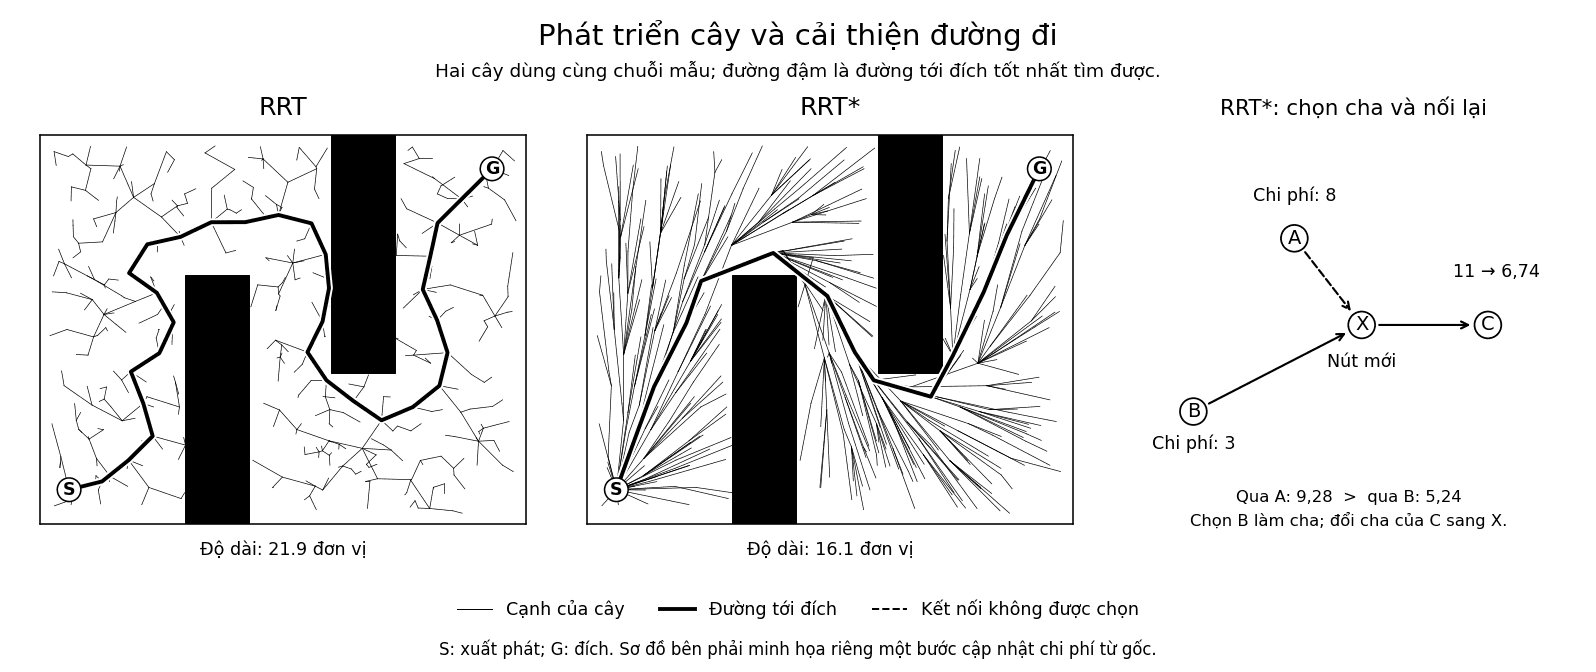
\includegraphics[width=\linewidth]{so_sanh_rrt_rrt_star.png}
    \chuthichhinh[fig:so-sanh-rrt-rrt-star]{Phát triển cây và cải thiện đường đi của RRT, RRT*}
  \end{center}
\end{minipage}\par\medskip

\subsubsection*{c. Tính tối ưu tiệm cận và ý nghĩa triển khai}

Nếu \(J_N\) là chi phí lời giải tốt nhất sau quá trình mở rộng và \(J^{*}\) là chi phí tối ưu của bài toán, tính tối ưu tiệm cận được biểu diễn bởi
\begin{equation}
  \mathbb{P}\!\left(\lim_{N\to\infty}J_N=J^{*}\right)=1.
  \label{eq:rrtstar-optimality}
\end{equation}
Đối với RRT*, khẳng định này gắn với các giả thiết về miền tự do, đường khả thi có khoảng hở thích hợp, hàm chi phí, quy tắc lấy mẫu, bán kính kết nối và bộ nối cục bộ. Nó không có nghĩa đường tìm được sau một số mẫu hữu hạn đã tối ưu, cũng không xác định một thời gian chờ cố định để đạt sai số mong muốn \cite{karaman-frazzoli-2011}.

So với RRT, RRT* phải xét thêm các láng giềng và kiểm tra nhiều kết nối, nên chất lượng đường đi được đánh đổi với thời gian tính toán. Tìm láng giềng, kiểm tra va chạm và cập nhật cây đều ảnh hưởng đến thời gian thực tế. Khi so sánh trong mô phỏng, cần dùng cùng bản đồ và ngân sách tính toán, chạy nhiều lần với các hạt giống ngẫu nhiên khác nhau, đồng thời báo cáo tỷ lệ thành công và chi phí lời giải. Đường gấp khúc tìm được vẫn phải được xử lý để đáp ứng giới hạn vận tốc, gia tốc và độ cong của robot.

\section{Nhóm Thuật toán Dựa trên Trường Lực (Potential Field Planning)}

Nhóm phương pháp trường lực tạo một trường hướng chuyển động từ thông tin vị trí đích và vật cản. Thay vì duyệt một đồ thị hoặc phát triển một cây trước khi có đường đi, robot cập nhật hướng đi theo trạng thái hiện tại. Cách tiếp cận này phù hợp với phản ứng cục bộ, nhưng cần phân tích các điểm cân bằng của trường để đánh giá khả năng tới đích.

\subsection{Phương pháp Trường Thế Nhân Tạo (APF)}

\subsubsection*{a. Mô hình và hàm thế hút}

APF (Artificial Potential Field) mô hình hóa đích như nguồn hút và vật cản như nguồn đẩy. Trong mô hình hai chiều, đặt \(\mathbf{q}=[x,y]^{T}\), \(\mathbf{q}_g=[x_g,y_g]^{T}\). Robot được xem là điểm sau khi đã tính đến kích thước thân xe bằng vùng cấm tương ứng. Hàm thế tổng hợp được xây dựng từ thế hút và tổng các thế đẩy \cite{khatib-apf-1986}:
\begin{equation}
  U(\mathbf{q})=U_{\mathrm{att}}(\mathbf{q})
    +\sum_{i=1}^{M}U_{\mathrm{rep},i}(\mathbf{q}),
  \label{eq:apf-potential}
\end{equation}
trong đó \(M\) là số vật cản được xét. Một thế hút dạng bậc hai là
\begin{equation}
  U_{\mathrm{att}}(\mathbf{q})
    =\frac{1}{2}k_{\mathrm{att}}\|\mathbf{q}-\mathbf{q}_g\|^{2},
  \qquad k_{\mathrm{att}}>0.
\end{equation}
Lực hút ảo bằng âm gradient của thế hút:
\begin{equation}
  \mathbf{F}_{\mathrm{att}}(\mathbf{q})
    =-\nabla U_{\mathrm{att}}(\mathbf{q})
    =k_{\mathrm{att}}(\mathbf{q}_g-\mathbf{q}).
  \label{eq:apf-attractive-force}
\end{equation}
Lực này hướng tới đích và giảm độ lớn khi khoảng cách đến đích giảm. Khi đưa vào bộ điều khiển, cần giới hạn vận tốc tham chiếu để tránh việc lực lớn ở xa đích tạo ra lệnh chuyển động vượt giới hạn của xe.

\subsubsection*{b. Hàm thế đẩy và đạo hàm gradient}

Gọi \(\rho_i(\mathbf{q})>0\) là khoảng cách ngắn nhất từ cấu hình điểm đến biên vùng cấm của vật cản thứ \(i\), \(\rho_0>0\) là khoảng tác động. Một dạng thế đẩy thường dùng là
\begin{equation}
  U_{\mathrm{rep},i}(\mathbf{q})=
  \begin{cases}
    \displaystyle\frac{1}{2}k_{\mathrm{rep},i}
      \left(\frac{1}{\rho_i(\mathbf{q})}-\frac{1}{\rho_0}\right)^{2},
      &0<\rho_i(\mathbf{q})<\rho_0,\\[6pt]
    0,&\rho_i(\mathbf{q})\geq\rho_0,
  \end{cases}
  \label{eq:apf-repulsive-potential}
\end{equation}
với \(k_{\mathrm{rep},i}>0\). Vật cản ngoài khoảng tác động không đóng góp lực đẩy; khi robot tiến sát vùng cấm, giá trị thế tăng mạnh. Công thức được xét trong miền tự do và không được tính bằng cách chia cho khoảng cách bằng \(0\).

Tại những điểm mà hàm khoảng cách khả vi, áp dụng quy tắc đạo hàm hàm hợp thu được
\begin{equation}
  \mathbf{F}_{\mathrm{rep},i}(\mathbf{q})=
  \begin{cases}
    \displaystyle k_{\mathrm{rep},i}
      \left(\frac{1}{\rho_i(\mathbf{q})}-\frac{1}{\rho_0}\right)
      \frac{\nabla\rho_i(\mathbf{q})}{\rho_i^{2}(\mathbf{q})},
      &0<\rho_i(\mathbf{q})<\rho_0,\\[6pt]
    \mathbf{0},&\rho_i(\mathbf{q})\geq\rho_0.
  \end{cases}
  \label{eq:apf-repulsive-force}
\end{equation}
Nếu \(\mathbf{q}_{\mathrm{obs},i}\) là điểm biên gần nhất duy nhất, thì
\[
  \nabla\rho_i(\mathbf{q})=
    \frac{\mathbf{q}-\mathbf{q}_{\mathrm{obs},i}}{\rho_i(\mathbf{q})},
\]
nên lực đẩy có hướng từ vật cản ra phía robot. Tại các điểm có nhiều điểm biên gần nhất hoặc trên bản đồ khoảng cách rời rạc, cần lựa chọn cách tính hướng nhất quán, vì gradient có thể không duy nhất hoặc chịu nhiễu do độ phân giải.

\subsubsection*{c. Lực tổng hợp và cập nhật chuyển động}

Lực ảo tổng hợp là
\begin{equation}
  \mathbf{F}_{\mathrm{total}}(\mathbf{q})
    =-\nabla U(\mathbf{q})
    =\mathbf{F}_{\mathrm{att}}(\mathbf{q})
      +\sum_{i=1}^{M}\mathbf{F}_{\mathrm{rep},i}(\mathbf{q}).
  \label{eq:apf-total-force}
\end{equation}
Trong mô phỏng điểm hình học, có thể thử cập nhật \(\mathbf{q}_{k+1}=\mathbf{q}_k+\alpha_k\mathbf{F}_{\mathrm{total}}(\mathbf{q}_k)\), với \(\alpha_k>0\) là hệ số bước. Trước khi chấp nhận, phải kiểm tra toàn bộ đoạn chuyển động; nếu đoạn đi vào vùng cấm thì giảm bước hoặc loại cập nhật. Lực đẩy lớn không tự bảo đảm một bước rời rạc không đi xuyên qua vật cản.

\noindent\begin{minipage}{\linewidth}
  \begin{center}
    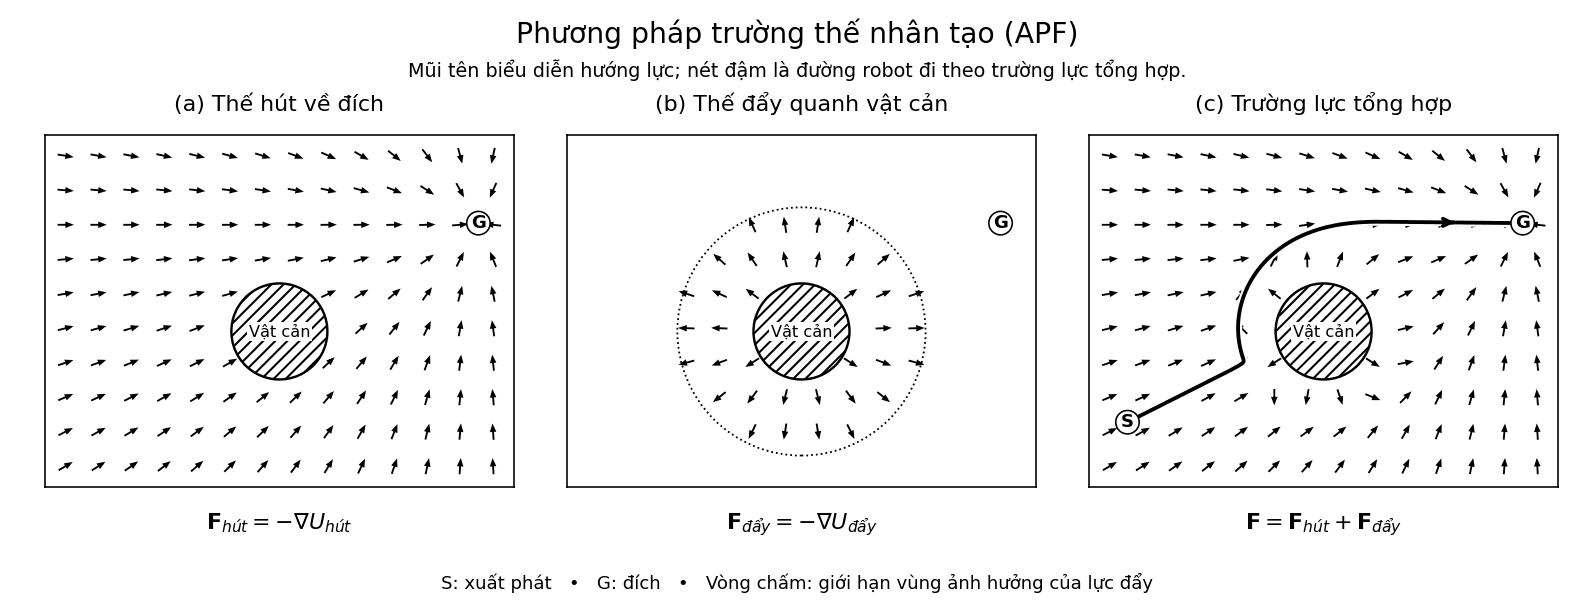
\includegraphics[width=\linewidth]{apf_the_hut_the_day_truong_luc.png}
    \chuthichhinh[fig:apf-the-hut-the-day]{Thế hút, thế đẩy và trường lực tổng hợp của APF}
  \end{center}
\end{minipage}\par\medskip

Trong ứng dụng cho robot vi sai, \(\mathbf{F}_{\mathrm{total}}\) là hướng dẫn chuyển động và không phải lực cơ học được áp trực tiếp lên thân xe. Xe chỉ có thể tạo vận tốc dọc thân và vận tốc góc; vì vậy cần chuyển hướng trường lực thành hướng mong muốn, sau đó dùng bộ điều khiển phù hợp để tạo lệnh vận tốc có giới hạn. Việc đánh giá tránh va chạm phải dựa trên chuyển động thực sự của xe, không chỉ dựa trên một mô hình điểm di chuyển tự do theo hai phương.

Tham số \(k_{\mathrm{att}}\), \(k_{\mathrm{rep},i}\) và \(\rho_0\) chi phối sự cân bằng giữa hướng đích và tránh vật cản. Chọn khoảng tác động quá lớn có thể làm robot khó đi qua hành lang, còn quá nhỏ có thể khiến phản ứng tránh vật cản xuất hiện muộn. Các tham số phải được kiểm tra cùng tốc độ chuyển động, độ trễ cảm biến và khoảng cách an toàn; không có một bộ giá trị tối ưu chung cho mọi bản đồ.

\subsection{Cực tiểu cục bộ, GNRON và lực ảo điều hướng}

\subsubsection*{a. Hiện tượng cực tiểu cục bộ}

Một vị trí \(\mathbf{q}_{\ell}\neq\mathbf{q}_g\) là cực tiểu cục bộ nếu thế tại đó nhỏ hơn hoặc bằng thế ở các vị trí lân cận. Khi hàm thế khả vi, điều kiện cần là \(\nabla U(\mathbf{q}_{\ell})=\mathbf{0}\), tương đương \(\mathbf{F}_{\mathrm{total}}(\mathbf{q}_{\ell})=\mathbf{0}\). Điều kiện gradient bằng \(0\) riêng lẻ chưa đủ để phân biệt cực tiểu với điểm yên ngựa hoặc cực đại; trong trường hợp khả vi hai lần, ma trận Hessian xác định dương là một điều kiện đủ cho cực tiểu nghiêm ngặt.

Trong bản đồ có vật cản dạng chữ U hoặc bố trí gần đối xứng, lực hút tới đích có thể bị các lực đẩy cân bằng ở một vị trí chưa tới đích. Robot đi theo âm gradient sẽ dừng hoặc dao động quanh vị trí đó. Nguyên nhân là APF cơ bản chỉ dùng hướng giảm thế tại chỗ, trong khi đường thoát khỏi một vùng bẫy có thể cần tạm thời đi xa đích hoặc tăng thế.

Trong cài đặt rời rạc, có thể đánh dấu nghi ngờ mắc kẹt nếu robot còn cách đích nhiều hơn dung sai, nhưng lực tổng hợp nhỏ, độ dịch chuyển rất nhỏ trong nhiều bước hoặc vị trí lặp lại. Các ngưỡng này cần được chọn theo thang đo và tốc độ của mô phỏng. Đây là tiêu chí phát hiện thực dụng, không phải phép chứng minh rằng vị trí đang xét là một cực tiểu toán học.

\subsubsection*{b. Mục tiêu không tiếp cận được khi có vật cản gần đích (GNRON)}

GNRON (Goals Nonreachable with Obstacles Nearby) xảy ra khi đích hợp lệ nằm trong vùng tác động của một vật cản, khiến lực đẩy vẫn tồn tại khi robot tiến tới đích. Với thế hút bậc hai, \(\mathbf{F}_{\mathrm{att}}(\mathbf{q}_g)=\mathbf{0}\); trong khi đó, thế đẩy truyền thống có thể tạo \(\mathbf{F}_{\mathrm{rep}}(\mathbf{q}_g)\neq\mathbf{0}\). Do đó, đích không còn là điểm cân bằng mong muốn của trường tổng hợp. Tình huống này có thể xảy ra khi robot cần tiếp cận một vị trí gần tường hoặc gần kệ hàng \cite{ge-cui-2000}.

Một cách sửa là làm thế đẩy phụ thuộc thêm khoảng cách tới đích. Đặt \(d_g=\|\mathbf{q}-\mathbf{q}_g\|\); trong khoảng tác động của vật cản, chọn dạng bậc hai theo khoảng cách đích:
\begin{equation}
  \widetilde{U}_{\mathrm{rep},i}(\mathbf{q})
    =\frac{1}{2}k_{\mathrm{rep},i}
      \left(\frac{1}{\rho_i(\mathbf{q})}-\frac{1}{\rho_0}\right)^{2}
      d_g^{2}.
  \label{eq:gnron-modified-potential}
\end{equation}
Ngoài khoảng tác động, thế sửa đổi bằng \(0\). Khi đích có khoảng hở dương tới vật cản, thế này và lực tương ứng tiến về \(0\) tại đích. Do thế hút chỉ bằng \(0\) tại đích và các thế đẩy không âm, đích trở thành cực tiểu toàn cục có giá trị thế bằng \(0\). Tuy vậy, vẫn có thể tồn tại các cực tiểu cục bộ khác; sửa GNRON không đồng nghĩa giải quyết mọi tình huống mắc kẹt \cite{ge-cui-2000}.

Để tính lực đúng, phải đạo hàm cả khoảng cách đến vật cản và khoảng cách đến đích. Đặt \(A_i=1/\rho_i-1/\rho_0\); trong miền \(0<\rho_i<\rho_0\), với \(d_g>0\), ta có
\begin{equation}
  \widetilde{\mathbf{F}}_{\mathrm{rep},i}
    =k_{\mathrm{rep},i}\frac{A_i d_g^{2}}{\rho_i^{2}}\nabla\rho_i
      -k_{\mathrm{rep},i}A_i^{2}d_g\nabla d_g.
  \label{eq:gnron-modified-force}
\end{equation}
Thành phần đầu đẩy robot ra khỏi vật cản; thành phần thứ hai có hướng tới đích do \(\nabla d_g\) hướng từ đích ra robot. Tại đích, sử dụng biểu thức theo vectơ hoặc giá trị giới hạn bằng \(\mathbf{0}\), tránh tính một vectơ đơn vị bằng cách chia cho \(d_g=0\). Biện pháp này chỉ xét đích nằm trong miền tự do; không thể biến một đích ở trong vùng cấm thành vị trí tiếp cận an toàn.

\hinhminhhoa[Cực tiểu cục bộ và hiện tượng GNRON]{Hình minh họa hai tình huống: robot mắc tại cực tiểu trước vật cản chữ U và robot không tới được đích gần vật cản do GNRON}

\subsubsection*{c. Giải pháp bổ sung lực ảo điều hướng}

Để hỗ trợ thoát bẫy, có thể bổ sung tạm thời một thành phần điều hướng khi phát hiện mắc kẹt. Một phương án đề xuất cho mô phỏng của đề tài là dùng hướng tiếp tuyến quanh vật cản đang chi phối. Gọi \(\mathbf{n}\) là hướng đơn vị đi ra khỏi vật cản; trong mặt phẳng, đặt
\begin{equation}
  \mathbf{t}_{\sigma}=\sigma
  \begin{bmatrix}
    0&-1\\ 1&0
  \end{bmatrix}\mathbf{n},\qquad \sigma\in\{-1,+1\},
  \qquad \mathbf{F}_{\mathrm{virt}}=k_{\mathrm{virt}}\mathbf{t}_{\sigma}.
  \label{eq:apf-virtual-force}
\end{equation}
Hai giá trị \(\sigma\) biểu diễn hai chiều vòng quanh vật cản. Hướng đi được tạo từ \(\mathbf{F}_{\mathrm{cmd}}=\mathbf{F}_{\mathrm{total}}+\mathbf{F}_{\mathrm{virt}}\). Đây là một quy tắc hỗ trợ cục bộ cần kiểm chứng trong mô phỏng, không phải một bảo đảm đầy đủ hoặc tối ưu của APF.

Quy trình dự kiến gồm phát hiện mắc kẹt, chọn vật cản gần đang chi phối, thử hai hướng thoát và kiểm tra tính khả thi của các bước ứng viên. Có thể ưu tiên hướng có khoảng hở tốt hơn hoặc phù hợp với đường tham chiếu toàn cục. Sau khi chọn, giữ hướng vòng trong một khoảng xử lý để hạn chế đổi chiều liên tục. Khi robot đã tiến bộ trở lại và thoát vùng bẫy, giảm rồi ngừng thành phần lực ảo; nếu không cải thiện trong ngân sách cho phép thì đổi điểm dẫn đường hoặc yêu cầu lập kế hoạch lại.

\hinhminhhoa[Lực ảo tiếp tuyến hỗ trợ thoát cực tiểu cục bộ]{Hình minh họa lực hút, lực đẩy và lực ảo tiếp tuyến giúp robot đổi hướng vòng qua vật cản khi bị mắc kẹt}

Lực ảo có thể phá vỡ trạng thái cân bằng nhưng cũng có thể dẫn robot sang một vùng khó khác. Khi thêm thành phần tiếp tuyến, trường điều hướng không nhất thiết còn là âm gradient của một hàm thế vô hướng, nên không thể dùng trực tiếp lập luận thế giảm đơn điệu của APF ban đầu. Mọi bước chuyển động vẫn cần giới hạn tốc độ, kiểm tra va chạm và theo dõi tiến triển tới đích.

Đối với đề tài robot ba bánh, một kiến trúc có thể khảo sát là dùng A*, PRM hoặc RRT* để tạo đường toàn cục, sau đó dùng APF để điều chỉnh hướng chuyển động cục bộ theo các điểm dẫn đường. Cách kết hợp này phải được đánh giá bằng các kịch bản có hành lang hẹp, vật cản chữ U và đích gần vật cản. Các kết quả về tỷ lệ thành công, chiều dài đường đi và thời gian xử lý chỉ được kết luận sau mô phỏng hoặc thực nghiệm; phần lý thuyết ở đây không giả định sẵn hiệu quả của phương án.

\section{Xây dựng Kịch bản Mô phỏng và Đánh giá So sánh Đa Thuật toán}

\subsection{Thiết lập môi trường mô phỏng trên nền tảng Python/MATLAB: Bản đồ không vật cản, Bản đồ mê cung tĩnh ô lưới, Bản đồ mật độ chướng ngại vật cao.}

\subsection{Bảng ma trận so sánh định lượng đa kịch bản giữa A*, PRM, RRT*, APF theo 4 chỉ số cốt lõi:}

\begin{itemize}

\item Chiều dài đường đi (m).

\item Thời gian xử lý tính toán CPU (ms).

\item Độ trơn của quỹ đạo (Tích phân độ cong \(\int \kappa {\left( s \right)}^{2}ds\)).

\item Tỷ lệ thành công tránh va chạm (\%).

\end{itemize}

\subsection{Bàn luận kết quả và lựa chọn bộ giải thuật quy hoạch tối ưu để triển khai xuống hệ thống phần cứng thực tế.}

\chapter{TRIỂN KHAI THỰC NGHIỆM TRÊN ROBOT 3 BÁNH, ĐÁNH GIÁ KẾT QUẢ VÀ ĐỀ XUẤT ỨNG DỤNG}

% Phông ký hiệu kỹ thuật có sẵn trên máy biên dịch.
\setmonofont{Consolas}

Chương này trình bày phương án tích hợp các thuật toán đã nghiên cứu lên robot vi sai ba bánh sử dụng ESP32-C3-MINI, mạch công suất TB6612, hai động cơ DC giảm tốc GA12-N20 có encoder Hall và bánh xe cao su đường kính \(44\,\mathrm{mm}\). Nội dung tập trung vào xây dựng phản hồi vận tốc, ước lượng tư thế, điều khiển bám đường và tổ chức thí nghiệm để đánh giá khả năng thực thi quỹ đạo.

Thông số linh kiện trong chương được ghi theo cấu hình được cung cấp; các giá trị tính toán từ thông số danh định được phân biệt với kết quả đo. Hiện chưa có nhật ký chạy thử, kích thước đầy đủ của khung xe hoặc dữ liệu định vị đối chứng. Vì vậy, phần thực nghiệm trình bày quy trình, tiêu chí và bảng ghi kết quả; các ô ``Chưa đo'' cần được thay bằng số liệu thực tế trước khi đưa ra kết luận định lượng.

\section{Thiết kế Hệ thống Phần cứng Robot 3 Bánh Thực nghiệm}

\subsection{Thiết kế cơ khí khung xe vi sai 3 bánh (2 bánh dẫn động chủ động độc lập + 1 bánh tự lựa Caster Wheel)}

\subsubsection*{a. Cấu hình cơ khí và thông số truyền động}

Hai động cơ được bố trí đối xứng qua trục dọc, mỗi động cơ dẫn động một bánh độc lập. Bánh tự lựa tạo điểm đỡ thứ ba và đổi hướng theo chuyển động của thân xe. Điểm tham chiếu \(P\) đặt tại trung điểm trục nối hai bánh chủ động; trục \(X_R\) hướng về phía trước, \(Y_R\) hướng sang trái, chiều quay dương ngược chiều kim đồng hồ. Cách chọn này thống nhất với mô hình động học ở Chương 2.

Động cơ có tên thương mại GA12 N20 Servo nhưng được sử dụng ở đây như động cơ DC giảm tốc có phản hồi encoder; vị trí hoặc vận tốc phải được điều khiển bằng vòng kín bên ngoài. Trục chữ D đường kính \(3\,\mathrm{mm}\) phù hợp với lỗ lắp bánh đã chọn. Các thông số công bố của động cơ và bánh xe được tổng hợp trong Bảng~\ref{tab:robot-hardware-specs}.

\begin{center}
\begin{minipage}{\linewidth}
  \centering
  \refstepcounter{table}\label{tab:robot-hardware-specs}%
  \tablename~\thetable: Thông số cấu hình robot theo thông tin được cung cấp\par\smallskip
  \small
  \renewcommand{\arraystretch}{1.25}
  \begin{tabular}{@{}p{0.49\linewidth}p{0.45\linewidth}@{}}
    \toprule
    \textbf{Hạng mục} & \textbf{Thông số}\\
    \midrule
    Vi điều khiển / driver động cơ & ESP32-C3-MINI / TB6612\\
    Loại động cơ & DC giảm tốc kim loại GA12-N20\\
    Điện áp hoạt động được cung cấp & \(3\)--\(12\,\mathrm{VDC}\)\\
    Tỷ số truyền hộp số & \(G=50:1\)\\
    Tốc độ trục động cơ trước giảm tốc & \(15\,000\,\mathrm{RPM}\)\\
    Tốc độ đầu ra không tải tại \(6\,\mathrm{VDC}\) & \(300\,\mathrm{RPM}\)\\
    Tốc độ đầu ra tải định mức được cung cấp & \(250\,\mathrm{RPM}\)\\
    Dòng không tải / tải định mức / kẹt trục & \(50/95/400\,\mathrm{mA}\)\\
    Mô-men định mức / kẹt trục & \(0.35/1.30\,\mathrm{kgf\cdot cm}\)\\
    Hộp số / khối lượng động cơ & \(12\times10\,\mathrm{mm}\) / khoảng \(10\,\mathrm{g}\)\\
    Trục đầu ra & Chữ D, đường kính \(3\,\mathrm{mm}\), dài \(10\,\mathrm{mm}\)\\
    Encoder & Hall hai kênh A/B; nguồn \(3.3\)--\(5\,\mathrm{VDC}\)\\
    Số chu kỳ mỗi kênh trên một vòng trục encoder & \(7\), trước hộp số\\
    Bánh xe & Cao su, đường kính \(44\,\mathrm{mm}\), rộng \(18\,\mathrm{mm}\)\\
    Bán kính bánh danh định & \(r_0=22\,\mathrm{mm}=0.022\,\mathrm{m}\)\\
    Khoảng cách tâm hai bánh chủ động \(L\) & Chưa đo\\
    Khối lượng robot và tải mang & Chưa đo\\
    \bottomrule
  \end{tabular}
\end{minipage}
\end{center}

Các giá trị tốc độ, dòng điện và mô-men trong bảng cần được kiểm chứng theo điều kiện cấp nguồn và tải của đúng động cơ đang dùng; chưa mặc nhiên coi tất cả là cùng một điểm làm việc đã được đo. Riêng từ đường kính bánh và tốc độ trục đầu ra, có thể tính tốc độ dài danh định:
\begin{equation}
  v=\frac{\pi D n}{60},\qquad D=0.044\,\mathrm{m}.
\end{equation}
Với \(n=250\,\mathrm{RPM}\), kết quả là khoảng \(0.576\,\mathrm{m/s}\); với \(300\,\mathrm{RPM}\), kết quả là khoảng \(0.691\,\mathrm{m/s}\). Đây là phép quy đổi hình học, không phải tốc độ vận hành đã xác nhận của robot. Giới hạn điều khiển cần được chọn sau khi đo đáp ứng dưới tải, có dự phòng cho chuyển hướng và giảm tốc.

\subsubsection*{b. Bố trí khung xe và hiệu chuẩn hình học}

Khung cần giữ hai trục động cơ thẳng hàng, hai bánh tiếp xúc đều và moay-ơ không trượt trên trục. Pin và mạch điều khiển được bố trí để trọng tâm nằm trong vùng đỡ của ba bánh, đồng thời không làm giảm quá mức lực ép lên bánh chủ động. Bánh tự lựa cần quay tự do; độ rơ, ma sát hoặc lệch lắp ráp của bánh này có thể làm thay đổi tải khi xe chuyển hướng.

Trước khi chạy thuật toán, đo \(L\) giữa tâm hai vệt tiếp xúc bánh chủ động, đo đường kính lăn khi có tải và kiểm tra dấu quay của từng bánh. Trong tính toán thực nghiệm, có thể dùng hai bán kính hiệu dụng \(r_L,r_R\) để phản ánh sai lệch lốp và lắp ráp; giá trị ban đầu đều lấy bằng \(r_0\), sau đó hiệu chỉnh qua các lượt đi thẳng và quay có đo đối chứng. Kích thước bao thân xe và phần nhô ra phải được đưa vào phép mở rộng vật cản, thay vì chỉ dùng đường kính bánh.

\hinhminhhoa[Bố trí cơ khí của robot ba bánh thực nghiệm]{Ảnh robot ba bánh thực nghiệm và bản vẽ bố trí hai động cơ N20, bánh cao su \(44\,\mathrm{mm}\), bánh tự lựa, điểm \(P\) và khoảng cách hai bánh \(L\)}

\subsection{Thiết kế mạch điện tử và phần cứng điều khiển: ESP32-C3-MINI, driver TB6612 và động cơ DC kèm encoder Hall hai kênh A/B}

\subsubsection*{a. Kiến trúc điều khiển và kết nối tín hiệu}

ESP32-C3-MINI đảm nhiệm thu nhận encoder, tính vận tốc bánh, cập nhật Odometry và thực hiện hai bộ điều khiển tốc độ. Thuật toán tìm đường và làm mượt có thể chạy trên máy tính, sau đó gửi đường tham chiếu hoặc các điểm dẫn đường tới robot. Đây là phương án phân chia đề xuất để giảm khối lượng tính toán trong vòng điều khiển; việc chạy trực tiếp toàn bộ bộ quy hoạch trên vi điều khiển cần được đánh giá riêng về bộ nhớ và thời gian xử lý.

Phương án đấu nối sử dụng hai ngõ PWM cho hai kênh công suất, bốn ngõ xác định chiều quay, một tín hiệu cho phép hoạt động và bốn ngõ vào encoder. Các chân GPIO cụ thể chỉ được chốt sau khi đối chiếu sơ đồ đúng phiên bản bo ESP32-C3-MINI, các chân phục vụ khởi động, nạp chương trình và giao tiếp. PWM được tạo bằng ngoại vi LEDC; encoder được đọc bằng ngắt GPIO theo tài liệu ESP-IDF dành cho ESP32-C3 \cite{espressif-c3-peripherals}.

Với module TB6612 sử dụng IC TB6612FNG, nguồn logic \(V_{CC}\) có dải hoạt động \(2.7\)--\(5.5\,\mathrm{V}\), nguồn động cơ \(V_M\) có dải \(2.5\)--\(13.5\,\mathrm{V}\). Phương án chọn \(V_{CC}=3.3\,\mathrm{V}\) để ghép mức logic; nguồn động cơ khởi đầu ở \(6\,\mathrm{V}\) theo điều kiện tốc độ không tải được cung cấp. Hai kênh dùng \texttt{AIN1/AIN2/PWMA} và \texttt{BIN1/BIN2/PWMB}; \texttt{STBY} mức thấp đưa IC về chờ. Chế độ phanh ngắn mạch và chế độ đầu ra trở kháng cao cần được phân biệt theo bảng chức năng của nhà sản xuất \cite[tr. 3--5]{toshiba-tb6612fng}.

Encoder được đề xuất cấp \(3.3\,\mathrm{V}\) và kiểm tra dạng tín hiệu A/B trước khi nối GPIO. Nếu cấp encoder bằng nguồn khác, cần xác nhận mức ngõ ra và phương án chuyển mức phù hợp với ESP32-C3. Nguồn động cơ và nguồn logic dùng chung điểm tham chiếu GND, có lọc nhiễu và bố trí đường cấp dòng động cơ tách khỏi đường tín hiệu encoder. Điện áp pin, dung lượng nguồn và cách hạ áp thực tế còn cần bổ sung vào hồ sơ lắp ráp.

\subsubsection*{b. Tổ chức phần mềm theo chu kỳ}

Vòng vận tốc chạy theo chu kỳ đặt trước \(T_s\); vòng bám đường có thể chạy chậm hơn, nhưng phải cấp lệnh kịp thời. Mỗi chu kỳ cần chụp đồng bộ bộ đếm hai bánh, tính thời gian thực đã trôi qua, cập nhật vận tốc và tư thế, tính điều khiển, xuất PWM rồi ghi dữ liệu vào bộ đệm. Truyền nhật ký ra máy tính được thực hiện ngoài trình phục vụ ngắt để tránh kéo dài thời gian xử lý xung.

Tần số PWM, độ phân giải duty, \(T_s\), chu kỳ bám đường và thời gian hết hạn lệnh là các tham số cấu hình phải ghi trong từng lượt thử. Chúng chưa được coi là số liệu đã chốt. Khi mất lệnh, dữ liệu tư thế quá cũ hoặc phát hiện lỗi đếm xung, chương trình chuyển về trạng thái dừng đã thiết kế; cách dừng được kiểm tra cùng driver và tải thực tế.

\hinhminhhoa[Sơ đồ kết nối phần cứng điều khiển và truyền động]{Sơ đồ kết nối ESP32-C3-MINI, TB6612, hai động cơ N20, encoder Hall A/B, các nhánh nguồn và đường truyền dữ liệu tới máy tính}

\subsection{Xây dựng thuật toán tính toán Odometry (Dead Reckoning) thời gian thực dựa trên đọc ngắt xung Encoder.}

\subsubsection*{a. Quy ước số đếm encoder và độ phân giải}

Theo mô tả được cung cấp, mỗi kênh A hoặc B có \(7\) chu kỳ xung trên một vòng trục trước hộp số. Với tỷ số truyền \(G=50\), một kênh tạo \(7\times50=350\) chu kỳ trên một vòng trục đầu ra. Số đếm dùng trong chương trình phụ thuộc cách giải mã, được phân biệt trong Bảng~\ref{tab:encoder-decoding}.

\begin{center}
\begin{minipage}{\linewidth}
  \centering
  \refstepcounter{table}\label{tab:encoder-decoding}%
  \tablename~\thetable: Số đếm danh định trên một vòng bánh xe\par\smallskip
  \renewcommand{\arraystretch}{1.3}
  \begin{tabular}{@{}p{0.13\linewidth}p{0.49\linewidth}p{0.27\linewidth}@{}}
    \toprule
    \textbf{Chế độ} & \textbf{Sự kiện được đếm} & \textbf{Số đếm/vòng bánh}\\
    \midrule
    x1 & Một cạnh của A; đọc B xác định chiều & \(N_{\mathrm{eff}}=350\)\\
    x2 & Cả hai cạnh của A; kết hợp trạng thái B & \(N_{\mathrm{eff}}=700\)\\
    x4 & Cả hai cạnh của cả A và B & \(N_{\mathrm{eff}}=1400\)\\
    \bottomrule
  \end{tabular}
\end{minipage}
\end{center}

Con số \(14\) xung trên một vòng trục encoder khi cộng số xung hai kênh tương ứng \(700\) sự kiện sau hộp số nếu chỉ tính một cạnh trên mỗi kênh; chưa phải phép giải mã x4. Không nhân thêm \(4\) nếu hằng số trong phần mềm đã là số đếm sau giải mã. Các giá trị trên dựa trên cách hiểu ``7 xung'' là 7 chu kỳ đầy đủ; trước khi sử dụng cần quay bánh một vòng có đánh dấu và đối chiếu số đếm thực.

Với \(r_0=0.022\,\mathrm{m}\), bước quãng đường danh định là
\begin{equation}
  \delta s=\frac{2\pi r_0}{N_{\mathrm{eff}}}.
  \label{eq:exp-encoder-step}
\end{equation}
Chế độ x1 cho khoảng \(0.395\,\mathrm{mm}\) mỗi đếm; x4 cho khoảng \(0.0987\,\mathrm{mm}\) mỗi đếm. Đây là độ phân giải lượng tử của phép đo, không đồng nghĩa với độ chính xác vị trí của robot.

Đọc x4 trên hai bánh ở tốc độ đầu ra \(300\,\mathrm{RPM}\) tạo tổng khoảng \(14\,000\) sự kiện mỗi giây theo thông số danh định. Vì vậy, trình phục vụ ngắt chỉ nên xác định chiều và cập nhật bộ đếm; khả năng không mất xung phải được kiểm tra khi chương trình đồng thời điều khiển và truyền dữ liệu. Phương án khởi đầu có thể dùng x1 rồi tăng độ phân giải nếu số liệu và tải xử lý cho phép.

\subsubsection*{b. Từ xung encoder đến độ dịch chuyển thân xe}

Gọi \(\Delta n_{L,k}\), \(\Delta n_{R,k}\) là số đếm có dấu trong chu kỳ thứ \(k\); chiều dương của cả hai bánh được quy ước làm robot tiến thẳng. Với \(N_L,N_R\) là số đếm hiệu dụng đã xác nhận,
\begin{equation}
  \Delta s_{L,k}=\frac{2\pi r_L\Delta n_{L,k}}{N_L},\qquad
  \Delta s_{R,k}=\frac{2\pi r_R\Delta n_{R,k}}{N_R}.
\end{equation}
Độ dịch chuyển trung bình và góc quay thân xe là
\begin{equation}
  \Delta s_k=\frac{\Delta s_{R,k}+\Delta s_{L,k}}{2},\qquad
  \Delta\theta_k=\frac{\Delta s_{R,k}-\Delta s_{L,k}}{L}.
  \label{eq:exp-odom-increments}
\end{equation}
Quan hệ này được suy ra từ mô hình vi sai; tích phân chuyển động bánh xe để ước lượng tư thế là nguyên lý của Odometry \cite[Mục 13.4]{lynch-park-modern-robotics}.

Nếu vận tốc xoắn của thân xe được coi là không đổi trong một chu kỳ, có thể cập nhật bằng công thức cung tròn:
\begin{equation}
  \begin{aligned}
    x_{k+1}&=x_k+\Delta s_k\operatorname{sinc}\!\left(\frac{\Delta\theta_k}{2}\right)
      \cos\left(\theta_k+\frac{\Delta\theta_k}{2}\right),\\
    y_{k+1}&=y_k+\Delta s_k\operatorname{sinc}\!\left(\frac{\Delta\theta_k}{2}\right)
      \sin\left(\theta_k+\frac{\Delta\theta_k}{2}\right),\\
    \theta_{k+1}&=\theta_k+\Delta\theta_k,
  \end{aligned}
  \label{eq:exp-odom-update}
\end{equation}
trong đó \(\operatorname{sinc}(z)=\sin z/z\), với \(\operatorname{sinc}(0)=1\). Khi góc nhỏ, dùng \(1-z^2/6\) để tránh chia cho số gần \(0\). Vận tốc đo được trong khoảng thời gian thực \(\Delta t_k\) là
\begin{equation}
  \widehat{v}_{L,k}=\frac{\Delta s_{L,k}}{\Delta t_k},\quad
  \widehat{v}_{R,k}=\frac{\Delta s_{R,k}}{\Delta t_k},\quad
  \widehat{v}_k=\frac{\Delta s_k}{\Delta t_k},\quad
  \widehat{\omega}_k=\frac{\Delta\theta_k}{\Delta t_k}.
\end{equation}

\subsubsection*{c. Xử lý số và hiệu chuẩn}

Các bộ đếm hai bánh cần được đọc trong cùng một vùng bảo vệ ngắn để hạn chế sai lệch thời điểm. Nếu dùng bộ đếm hữu hạn bit, phải tính chênh lệch có xét tràn; số đếm phát sinh giữa hai lần đọc phải nhỏ hơn nửa miền đếm để xác định được dấu. Với x4, có thể dùng bảng chuyển trạng thái A/B và ghi nhận các chuyển trạng thái không hợp lệ để phát hiện dấu hiệu mất xung hoặc nhiễu.

Ở vận tốc thấp, phép đếm trên cửa sổ thời gian ngắn có thể xen kẽ nhiều chu kỳ không có xung. Có thể tăng cửa sổ ước lượng, dùng bộ lọc vận tốc hoặc đo chu kỳ cạnh; lựa chọn phải cân bằng độ nhiễu và độ trễ của vòng PID. Phần cập nhật vị trí vẫn nên tích lũy từ số đếm gốc để không làm mất quãng đường do xử lý lọc.

Quy trình hiệu chuẩn gồm đi thẳng một quãng đo chuẩn để sửa tỷ lệ quãng đường, quay có đo góc để chỉnh \(L\), sau đó kiểm tra trên hành trình khép kín theo hai chiều quay. Các bộ \(r_L,r_R,L\), chế độ giải mã và phiên bản phần mềm phải được lưu cùng dữ liệu. Odometry tích lũy sai số do trượt bánh, biến dạng lốp và sai lệch kích thước; cần cảm biến hoặc phép đo độc lập khi đánh giá vị trí thực, thay vì dùng chính encoder làm chuẩn tuyệt đối.

\section{Thiết kế Kiến trúc Điều khiển Bám Quỹ đạo (Trajectory Tracking)}

Kiến trúc đề xuất gồm hai cấp: vòng ngoài tạo vận tốc thân xe \((v_c,\omega_c)\) từ đường tham chiếu và tư thế ước lượng; vòng trong điều khiển vận tốc từng bánh bằng PWM. Bộ quy hoạch, làm mượt và gán thời gian cung cấp dữ liệu tham chiếu; bộ bám không có nhiệm vụ tự tìm một đường tránh vật cản mới. Khi đường hiện tại không còn hợp lệ, phải dừng hoặc yêu cầu quy hoạch lại.

\hinhminhhoa[Kiến trúc điều khiển bám đường và tốc độ hai bánh]{Sơ đồ điều khiển hai cấp: quy hoạch và làm mượt, Pure Pursuit, chuyển đổi vận tốc hai bánh, hai bộ PID, TB6612 và phản hồi encoder/Odometry}

\subsection{\texorpdfstring{Thuật toán điều khiển hình học Pure Pursuit: Xác định tọa độ điểm nhìn trước \((L_{\mathrm{fw}})\) và công thức chuyển đổi bán kính cong sang tốc độ góc mong muốn \(\omega_c\).}{Thuật toán điều khiển hình học Pure Pursuit: Điểm nhìn trước và tốc độ góc mong muốn}}

\subsubsection*{a. Hình học điểm nhìn trước}

Pure Pursuit xác định một điểm phía trước trên đường và dựng cung tròn đi từ tư thế hiện tại tới điểm đó \cite[Mục 2--3]{coulter-pure-pursuit-1992}. Đặt tư thế ước lượng là \((\widehat{x},\widehat{y},\widehat{\theta})\), điểm nhìn trước trong hệ toàn cục là \((x_g,y_g)\). Chuyển điểm sang hệ thân xe:
\begin{equation}
  \begin{bmatrix}x_g^R\\y_g^R\end{bmatrix}
  =\begin{bmatrix}
    \cos\widehat{\theta}&\sin\widehat{\theta}\\
    -\sin\widehat{\theta}&\cos\widehat{\theta}
  \end{bmatrix}
  \begin{bmatrix}x_g-\widehat{x}\\y_g-\widehat{y}\end{bmatrix}.
\end{equation}
Trong quy ước \(X_R\) hướng trước, \(Y_R\) hướng trái, tâm cung tròn có tọa độ \((0,R_c)\). Điều kiện điểm nhìn trước nằm trên cung cho
\[
  (x_g^R)^2+(y_g^R-R_c)^2=R_c^2.
\]
Suy ra độ cong lệnh và vận tốc góc:
\begin{equation}
  \ell^2=(x_g^R)^2+(y_g^R)^2,\qquad
  \kappa_{\mathrm{pp}}=\frac{2y_g^R}{\ell^2},\qquad
  \omega_c=v_c\kappa_{\mathrm{pp}},\quad \ell>0.
  \label{eq:exp-pure-pursuit}
\end{equation}
Nếu điểm được chọn trên đường tròn nhìn trước bán kính \(L_{\mathrm{fw}}\), thì \(\ell=L_{\mathrm{fw}}\). Khi gần đích phải dùng khoảng cách thực \(\ell\), vì điểm cuối có thể nằm gần robot hơn bán kính đặt trước. Với \(y_g^R=0\), độ cong bằng \(0\) và robot đi thẳng; không cần tính bán kính vô hạn.

\subsubsection*{b. Phương án chọn điểm và giới hạn lệnh cho đề tài}

Đường tham chiếu được lưu theo thứ tự tiến triển từ đầu đến cuối. Tại mỗi chu kỳ, tìm điểm chiếu hoặc đoạn gần nhất trong cửa sổ quanh chỉ số đã đạt, sau đó tìm giao điểm phía trước với đường tròn nhìn trước. Cần chọn nhánh đúng theo thứ tự hành trình để tránh nhảy sang nhánh khác ở chỗ đường tự giao hoặc nằm gần nhau. Nếu không tìm được điểm phía trước hợp lệ, chuyển sang trạng thái xử lý mất đường; không tiếp tục dùng một chỉ số cũ không được kiểm tra.

Một luật chọn khoảng nhìn trước có thể khảo sát là
\begin{equation}
  L_{\mathrm{fw}}=\operatorname{clip}
  \bigl(L_0+k_v|\widehat{v}|,L_{\min},L_{\max}\bigr),
\end{equation}
với \(k_v\) có đơn vị giây. Các giá trị \(L_0,k_v,L_{\min},L_{\max}\) là tham số thử nghiệm, chưa có giá trị tối ưu được xác nhận. Cần khảo sát độ lệch ngang, dao động hướng và hiện tượng cắt góc khi thay đổi chúng ở cùng tốc độ và cùng bản đồ.

Tốc độ \(v_c\) lấy từ profile dọc đường nhưng phải được giới hạn theo độ cong lệnh \(\kappa_{\mathrm{pp}}\), tốc độ bánh và điều kiện giảm tốc. Gần đích, giảm tốc trước khi khoảng cách còn lại nhỏ hơn khoảng dừng cần thiết. Khi vị trí đã nằm trong dung sai và nhiệm vụ yêu cầu hướng cuối, dùng một pha căn chỉnh hướng riêng có giới hạn tốc độ quay; ở pha này không dùng phép chia \(\omega/v\). Phải đặt ngưỡng cho \(\ell\) để tránh chia cho số quá nhỏ trong \eqref{eq:exp-pure-pursuit}.

Lệnh vận tốc dài và vận tốc góc từng bánh là
\begin{equation}
  \begin{aligned}
    v_R^{\mathrm{ref}}&=v_c+\frac{L\omega_c}{2}, &
    v_L^{\mathrm{ref}}&=v_c-\frac{L\omega_c}{2},\\
    \omega_R^{\mathrm{ref}}&=\frac{v_R^{\mathrm{ref}}}{r_R}, &
    \omega_L^{\mathrm{ref}}&=\frac{v_L^{\mathrm{ref}}}{r_L}.
  \end{aligned}
\end{equation}
Nếu một bánh vượt giới hạn góc quay \(\Omega_{L,\max}\) hoặc \(\Omega_{R,\max}\), có thể giảm đồng thời hai lệnh bằng
\begin{equation}
  \gamma=\max\left\{1,
    \frac{|\omega_L^{\mathrm{ref}}|}{\Omega_{L,\max}},
    \frac{|\omega_R^{\mathrm{ref}}|}{\Omega_{R,\max}}\right\},
  \qquad
  (v_c,\omega_c)\leftarrow\frac{1}{\gamma}(v_c,\omega_c).
\end{equation}
Cách giảm chung này giữ tỷ lệ quay--tiến của lệnh tức thời. Sau đó vẫn cần giới hạn gia tốc và kiểm tra đoạn chuyển tiếp; chỉ cắt riêng vận tốc một bánh có thể làm đổi độ cong mong muốn.

Pure Pursuit trong cấu hình này chủ yếu bám hình học của đường. Nếu tốc độ được điều chỉnh theo tiến triển thực tế hoặc phải dừng do vật cản, robot có thể tới cùng vị trí ở thời điểm khác lịch tham chiếu ban đầu. Vì vậy, sai số bám đường và sai số bám theo thời gian phải được đánh giá riêng; không khẳng định thuật toán cơ bản bảo đảm đồng bộ thời gian với toàn bộ quỹ đạo.

\subsection{\texorpdfstring{Thiết kế bộ điều khiển PID vận tốc vòng kín (Closed-loop Speed Controller) điều chế PWM cho từng động cơ bánh trái/phải (\(v_{L},v_{R}\)).}{Thiết kế bộ điều khiển PID vận tốc vòng kín (Closed-loop Speed Controller) điều chế PWM cho từng động cơ bánh trái/phải (vL,vR).}}

\subsubsection*{a. Cấu trúc điều khiển rời rạc}

Hai bộ điều khiển nhận vận tốc dài tham chiếu \(v_i^{\mathrm{ref}}\) và vận tốc đo \(\widehat{v}_i\), với \(i\in\{L,R\}\). Sai số trong chu kỳ thứ \(k\) là
\begin{equation}
  e_{i,k}=v_{i,k}^{\mathrm{ref}}-\widehat{v}_{i,k}.
\end{equation}
Cấu trúc PID sử dụng thành phần tỷ lệ, tích phân và vi phân; tích phân cần xử lý bão hòa đầu ra để tránh tích lũy quá mức \cite{ros-control-pid}. Phương án đề xuất cho robot là PID có nhánh bù thuận và đạo hàm trên tín hiệu đo đã lọc:
\begin{equation}
  u_{i,k}^{*}=K_{\mathrm{ff},i}v_{i,k}^{\mathrm{ref}}
       +K_{P,i}e_{i,k}+I_{i,k}-K_{D,i}d_{i,k},
\end{equation}
\begin{equation}
  d_{i,k}=\rho_i d_{i,k-1}
    +(1-\rho_i)\frac{\widehat{v}_{i,k}-\widehat{v}_{i,k-1}}{\Delta t_k},
  \quad 0\leq\rho_i<1,
\end{equation}
\begin{equation}
  u_{i,k}=\operatorname{clip}(u_{i,k}^{*},-u_{\max,i},u_{\max,i}).
\end{equation}
Trong đó, \(u\) là duty có dấu đã chuẩn hóa, với \(0<u_{\max,i}\leq1\); dấu quyết định chiều quay và trị tuyệt đối quyết định duty PWM. Nếu chưa xác định được nhánh bù thuận, đặt \(K_{\mathrm{ff},i}=0\). Nếu tín hiệu đo còn nhiều nhiễu, có thể bắt đầu từ PI bằng cách đặt \(K_{D,i}=0\), sau đó đánh giá nhu cầu bổ sung vi phân.

Một cách chống bão hòa tích phân bằng hồi tiếp sai lệch đầu ra là
\begin{equation}
  I_{i,k+1}=\operatorname{clip}\!\left(
    I_{i,k}+\Delta t_k\left[
      K_{I,i}e_{i,k}+\frac{u_{i,k}-u_{i,k}^{*}}{T_{t,i}}
    \right],I_{\min,i},I_{\max,i}\right),
  \quad T_{t,i}>0.
  \label{eq:exp-pid-antiwindup}
\end{equation}
Thành phần hiệu chỉnh chỉ kéo tích phân về phía đầu ra đang thực hiện khi có bão hòa. Các giới hạn duty, tích phân và tốc độ thay đổi lệnh phải được xác định cùng tải thực tế; phép điều chế PWM không đồng nghĩa với một điện áp trung bình hoàn toàn tuyến tính ở mọi chế độ của driver.

\subsubsection*{b. Ghép với TB6612 và hiệu chỉnh tham số}

Mỗi kênh TB6612 được gán cho một động cơ, sau đó kiểm tra dấu PWM, dấu encoder và chiều tiến để bảo đảm phản hồi âm. Chế độ dừng, phanh và chờ được tách thành trạng thái rõ ràng; không coi mọi lệnh duty bằng \(0\) đều tương đương với thả trôi. Khi đổi chiều, lệnh được giảm có kiểm soát trước khi đảo dấu; không dùng đảo chiều đột ngột như cách hiệu chỉnh sai số tốc độ thông thường.

Quy trình hiệu chỉnh đề xuất bắt đầu từ đo quan hệ duty--tốc độ của từng bánh dưới tải để nhận biết vùng chết và mức bão hòa. Sau đó tăng dần \(K_P\), bổ sung \(K_I\) để giảm sai số xác lập, và chỉ dùng \(K_D\) khi có lợi sau khi lọc vận tốc. Hai bên có thể cần hệ số khác nhau do ma sát, tải hoặc động cơ khác nhau. Việc đánh giá gồm đáp ứng khởi động, thay đổi tốc độ, giảm về \(0\) và đảo chiều ở mức đã giới hạn.

Từng cấu hình được ghi các chỉ tiêu thời gian xác lập theo một dải dung sai đã chọn, độ quá điều chỉnh, sai số xác lập, độ nhiễu vận tốc và tỷ lệ thời gian bão hòa PWM. Khi đổi trạng thái dừng/chạy, cần khởi tạo hoặc giữ trạng thái tích phân theo quy tắc nhất quán để tránh bước nhảy điều khiển. Các giá trị \(K_P,K_I,K_D,T_t,\rho\) chưa được gán trước khi có dữ liệu đáp ứng.

\section{Kết quả Thực nghiệm Thực tế và Đánh giá Sai số}

Phần này quy định cách thu thập và trình bày kết quả. Do chưa có dữ liệu chạy robot, các bảng bên dưới là biểu mẫu thực nghiệm, chưa thể dùng để kết luận robot đã đạt độ chính xác hoặc tỷ lệ tránh va chạm cụ thể. Trước mỗi đợt đo cần chốt thông số \(L,r_L,r_R,N_L,N_R\), cấu hình điều khiển, tải, điện áp nguồn và điều kiện mặt sàn.

Một lượt thử gồm khởi tạo tư thế, kiểm tra dữ liệu, phát nhiệm vụ, ghi toàn bộ quá trình và lưu nguyên nhân kết thúc. Mỗi cấu hình được lặp với số lượt đã quy định trước; các lượt không tới đích, mất dữ liệu hoặc bị dừng phải được lưu lại cùng trạng thái, thay vì chỉ giữ các lượt thành công. Ngưỡng đạt/không đạt cần được xác định trước khi xem kết quả, dựa trên bề rộng hành lang, dung sai điểm dừng và khả năng đo của hệ thống.

\subsection{Kịch bản thực nghiệm 1: Kiểm thử khả năng bám quỹ đạo định sẵn (Đường thẳng và Đường cong S-Curve).}

\subsubsection*{a. Đường thẳng}

Đặt đường tham chiếu có chiều dài \(\ell_s\) trong vùng sàn phẳng được đo kích thước. Thực hiện lượt khởi đầu thẳng hàng để khảo sát sai lệch hai truyền động, rồi các lượt có lệch ngang hoặc lệch hướng ban đầu được xác định trước để khảo sát khả năng trở lại đường. Giữ nguyên tải, thông số PID, khoảng nhìn trước và giới hạn tốc độ trong các lượt cần so sánh.

Tốc độ dọc đường dùng profile tăng--giữ--giảm đã giới hạn ở Chương 2. Theo dõi vận tốc đặt/đo của từng bánh, duty PWM, tư thế Odometry và vị trí đối chứng. Dấu hiệu robot lệch liên tục về một phía cần được phân tích cùng bán kính lăn, hệ số truyền động và sai số định vị; không mặc nhiên sửa mọi sai lệch bằng cách tăng hệ số bám đường.

\subsubsection*{b. Đường cong chữ S}

Trong kịch bản này, chữ S mô tả hình dạng đường đi trong mặt phẳng, khác với profile vận tốc chữ S theo thời gian. Một đường thử có thể tự xây dựng là
\begin{equation}
  x_d(u)=\ell_s u,\qquad
  y_d(u)=A\left(10u^3-15u^4+6u^5\right),
  \quad 0\leq u\leq1,\quad \ell_s>0.
  \label{eq:exp-spatial-s-path}
\end{equation}
Biên độ \(A\) và chiều dài \(\ell_s\) được chọn sau khi đo mặt bằng. Đường có tiếp tuyến nằm ngang và độ cong bằng \(0\) tại hai đầu; có thể nối với các đoạn thẳng cùng hướng. Quy luật \(u(t)\) phải được chọn theo độ cong và giới hạn bánh, thay vì chỉ đặt tốc độ không đổi cho mọi hình dạng đường.

Các lượt khảo sát thay đổi từng yếu tố như mức tốc độ, tham số nhìn trước hoặc lựa chọn làm mượt, trong khi giữ các yếu tố khác cố định. Chỉ tiêu cần ghi gồm sai số ngang, sai số hướng, sai số dừng cuối, tốc độ/gia tốc bánh và thời gian hoàn thành. Nếu so sánh đường gấp khúc với đường mượt, phải nêu rõ phương án gấp khúc có dừng--xoay ở góc hay không, vì hai cách thực hiện có thể khác đáng kể về thời gian.

\hinhminhhoa[Bố trí thí nghiệm bám đường thẳng và đường cong chữ S]{Sơ đồ bố trí đường thẳng và đường cong chữ S trong phòng thí nghiệm, điểm đầu/cuối, các vị trí đo đối chứng và ảnh robot khi chạy thử}

\subsection{Kịch bản thực nghiệm 2: Tự hành tính toán và quy hoạch quỹ đạo né vật cản thực tế trong không gian phòng thí nghiệm.}

\subsubsection*{a. Thiết lập bản đồ và chuỗi xử lý}

Mặt bằng thử được đo trong cùng hệ tọa độ với vị trí robot và mục tiêu. Với cấu hình hiện được cung cấp chỉ có encoder, thí nghiệm cơ sở dùng vật cản tĩnh đã đo và nhập vào bản đồ; không giả định robot đã có khả năng tự phát hiện vật cản chưa biết. Phần nhô của thân xe được xét qua vùng cấm cho tâm robot, cộng khoảng dự phòng cho sai số định vị và sai số bám.

Chuỗi xử lý đề xuất gồm tạo bản đồ, chạy bộ tìm đường của Chương 3, kiểm tra đường nối, làm mượt theo mục 2.4, gán tốc độ khả thi rồi gửi đường cho bộ bám. Trước khi chạy, xác nhận đường mượt còn nằm trong vùng tự do. Trong lượt thử, robot đi theo đường đã duyệt; nếu sai lệch vượt miền cho phép hoặc xuất hiện tình huống không được bản đồ mô tả, lượt thử được dừng và ghi lý do.

\subsubsection*{b. Tổ chức so sánh và ghi nhận kết thúc}

Các thuật toán được so sánh trên cùng bản đồ, điểm đầu/đích, mô hình thân xe, quy tắc kiểm tra va chạm và giới hạn chuyển động. Với phương pháp ngẫu nhiên, lưu hạt giống và ngân sách tìm kiếm. Thời gian tính đường được đo trên đúng thiết bị thực thi bộ quy hoạch, tách khỏi thời gian truyền dữ liệu và thời gian robot di chuyển.

Có thể khảo sát ba bố trí: vật cản đơn để kiểm tra vòng tránh, nhiều vật cản để đánh giá đường toàn cục và hành lang hẹp để kiểm tra khoảng hở. Kích thước cụ thể phải được lưu cùng sơ đồ. Nếu nguồn lực chỉ cho phép thử một số bộ quy hoạch, báo cáo rõ nhóm đã thử; không suy rộng kết quả cho các thuật toán chỉ có phần mô phỏng.

Lượt thử được tính thành công khi robot đạt vùng đích theo dung sai đã đặt, hoàn thành yêu cầu hướng nếu có, không chạm vật cản và không cần can thiệp thủ công. Chỉ việc có một đường đi trên bản đồ chưa đủ để tính là một lượt robot thành công. Các lượt hết thời gian, lỗi điều khiển hoặc bị dừng cũng phải được phân loại.

\begin{center}
\begin{minipage}{\linewidth}
  \centering
  \refstepcounter{table}\label{tab:exp-result-template}%
  \tablename~\thetable: Biểu mẫu tổng hợp kết quả theo nhóm kịch bản\par\smallskip
  \small
  \renewcommand{\arraystretch}{1.35}
  \begin{tabular}{@{}p{0.35\linewidth}p{0.17\linewidth}p{0.17\linewidth}p{0.17\linewidth}@{}}
    \toprule
    \textbf{Chỉ tiêu} & \textbf{Đường thẳng} & \textbf{Chữ S} & \textbf{Có vật cản}\\
    \midrule
    Số lượt thử / số lượt thành công & Chưa đo & Chưa đo & Chưa đo\\
    RMSE vị trí đối chứng (m) & Chưa đo & Chưa đo & Chưa đo\\
    Sai số ngang lớn nhất (m) & Chưa đo & Chưa đo & Chưa đo\\
    Sai số hướng trung bình (rad) & Chưa đo & Chưa đo & Chưa đo\\
    Sai số vị trí cuối (m) & Chưa đo & Chưa đo & Chưa đo\\
    Thời gian hoàn thành (s) & Chưa đo & Chưa đo & Chưa đo\\
    Khoảng hở thân xe nhỏ nhất (m) & Không áp dụng & Không áp dụng & Chưa đo\\
    Tỷ lệ thời gian PWM bão hòa (\%) & Chưa đo & Chưa đo & Chưa đo\\
    \bottomrule
  \end{tabular}
\end{minipage}
\end{center}

Các hàng RMSE theo thời gian chỉ được điền khi có lịch tham chiếu tương ứng và dữ liệu đo đã đồng bộ. Mỗi bảng kết quả chính thức phải đi kèm cấu hình điều khiển và mô tả thiết bị đo; khi so sánh thuật toán, bổ sung cột hoặc bảng riêng cho từng bộ quy hoạch. Khoảng hở được tính từ biên thân xe tới vật cản, không chỉ từ điểm tâm robot.

\subsection{\texorpdfstring{Thu thập dữ liệu và biểu diễn sai số bám quỹ đạo \(\left( e_{x},e_{y},e_{\theta} \right)\) giữa quỹ đạo lý thuyết và quỹ đạo thực tế.}{Thu thập dữ liệu và biểu diễn sai số bám quỹ đạo ex,ey,eθgiữa quỹ đạo lý thuyết và quỹ đạo thực tế.}}

\subsubsection*{a. Ghi dữ liệu và thiết lập phép đo đối chứng}

Nhật ký tối thiểu cần có thời gian đo, số đếm encoder hai bánh, vận tốc đặt/đo, lệnh \(v_c,\omega_c\), duty PWM, tư thế Odometry, chỉ số tiến triển trên đường và trạng thái điều khiển. Hồ sơ lượt chạy ghi thêm thông số hình học, nguồn điện, tải, PID, khoảng nhìn trước, bản đồ, bộ quy hoạch và điều kiện kết thúc.

Để đánh giá vị trí thực, có thể dùng camera đã hiệu chuẩn quan sát dấu mốc trên robot, hệ theo dõi ngoài hoặc phép đo vị trí tại các mốc cố định. Gốc tọa độ, tỷ lệ chiều dài và độ lệch giữa dấu mốc đo với điểm \(P\) phải được xác định. Phép đo mốc rời rạc chỉ hỗ trợ đánh giá ở các vị trí đó; không đủ để suy ra RMSE liên tục toàn hành trình. Độ phân giải và độ không chắc chắn của phép đo cần được báo cáo cùng sai số robot.

Các chuỗi dữ liệu được chuyển về cùng hệ tọa độ và cùng lưới thời gian. Chỉ nội suy trong khoảng có dữ liệu hợp lệ, ghi lại khoảng mất mẫu và độ lệch đồng hồ. Không chỉnh lại gốc hay thời gian riêng cho từng đoạn để làm giảm sai số sau khi đã xem kết quả. Nếu chỉ có encoder, các đồ thị được ghi là sai số trên tư thế ước lượng; chúng chưa phải bằng chứng về độ chính xác vị trí thật.

\subsubsection*{b. Sai số theo thời gian và sai số hình học}

Gọi \((x_k^{\mathrm{gt}},y_k^{\mathrm{gt}},\theta_k^{\mathrm{gt}})\) là tư thế đối chứng và \((x_{d,k},y_{d,k},\theta_{d,k})\) là tham chiếu tại cùng thời điểm. Quy ước sai số là thực tế trừ tham chiếu:
\begin{equation}
  \begin{aligned}
    e_{x,k}&=x_k^{\mathrm{gt}}-x_{d,k},\\
    e_{y,k}&=y_k^{\mathrm{gt}}-y_{d,k},\\
    e_{\theta,k}&=\operatorname{atan2}
      \bigl(\sin(\theta_k^{\mathrm{gt}}-\theta_{d,k}),
            \cos(\theta_k^{\mathrm{gt}}-\theta_{d,k})\bigr).
  \end{aligned}
\end{equation}
Với \(N\) mẫu cách đều thời gian, một số chỉ tiêu là
\begin{equation}
  \operatorname{RMSE}_{p}=\sqrt{\frac{1}{N}\sum_{k=1}^{N}
    (e_{x,k}^{2}+e_{y,k}^{2})},\qquad
  E_{p,\max}=\max_k\sqrt{e_{x,k}^{2}+e_{y,k}^{2}},
\end{equation}
\begin{equation}
  \operatorname{MAE}_{\theta}=\frac{1}{N}\sum_{k=1}^{N}|e_{\theta,k}|.
\end{equation}
Các đại lượng này phản ánh cả sai lệch hình học và việc robot nhanh/chậm so với lịch. Để đánh giá riêng bám đường, tìm điểm chiếu \(\mathbf{p}(s_k^*)\) theo nhánh tiến triển hợp lệ và dùng hướng tiếp tuyến \(\theta_p(s_k^*)\). Sai số ngang có dấu là
\begin{equation}
  e_{\perp,k}=
    \begin{bmatrix}-\sin\theta_p(s_k^*)&\cos\theta_p(s_k^*)\end{bmatrix}
    \left(\begin{bmatrix}x_k^{\mathrm{gt}}\\y_k^{\mathrm{gt}}\end{bmatrix}
       -\mathbf{p}(s_k^*)\right).
\end{equation}
Sai số vị trí cuối được tính trực tiếp từ vị trí robot lúc kết thúc và điểm đích, không thay bằng sai số chiếu lên một đoạn bất kỳ. Nếu cần đánh giá riêng Odometry, so sánh tư thế Odometry với tư thế đối chứng cùng thời điểm, tách khỏi sai số giữa robot và đường tham chiếu.

\subsubsection*{c. Thống kê và cách trình bày kết quả}

Với \(n_{\mathrm{run}}\) lượt và \(n_{\mathrm{ok}}\) lượt thành công, tỷ lệ thành công là
\begin{equation}
  P_{\mathrm{ok}}=100\frac{n_{\mathrm{ok}}}{n_{\mathrm{run}}}\,\%,
  \qquad n_{\mathrm{run}}>0.
\end{equation}
Cho chỉ tiêu \(J_j\) của \(n\) lượt có dữ liệu hợp lệ, báo cáo trung bình và độ lệch chuẩn mẫu:
\begin{equation}
  \overline{J}=\frac{1}{n}\sum_{j=1}^{n}J_j,\qquad
  s_J=\sqrt{\frac{1}{n-1}\sum_{j=1}^{n}(J_j-\overline{J})^2},
  \quad n\geq2.
\end{equation}
Nếu thống kê chỉ dùng các lượt thành công, phải ghi rõ điều đó và vẫn công bố tỷ lệ thành công trên toàn bộ lượt thử. Lượt thất bại không được gán thời gian hay sai số bằng \(0\). Với so sánh theo cặp, dùng cùng bố trí và điều kiện khởi đầu để giảm ảnh hưởng của các yếu tố ngoài thuật toán.

Bộ hình kết quả nên gồm đường tham chiếu và đường đo trên mặt phẳng, đồ thị \(e_x,e_y,e_{\theta},e_{\perp}\), vận tốc hai bánh đặt/đo và duty PWM theo thời gian. Đánh dấu các thời điểm bão hòa, mất mẫu, đổi trạng thái hoặc dừng. Từ các đồ thị mới phân tích được sai số chủ yếu do định vị, bám đường, vòng tốc độ, độ trễ hay điều kiện tiếp xúc; chưa có dữ liệu thì chưa xếp hạng thuật toán hoặc khẳng định mức cải thiện.

\hinhminhhoa[Đồ thị quỹ đạo, sai số bám và đáp ứng truyền động]{Đồ thị kết quả cần bổ sung: đường tham chiếu và đường đo thực tế; sai số vị trí/hướng; vận tốc hai bánh đặt--đo và PWM theo thời gian}

\section{Đề xuất Hướng Ứng dụng Thực tế và Mở rộng Đề tài}

\subsection{Khả năng ứng dụng vào các dòng xe tự hành AGV/AMR vận chuyển hàng hóa thông minh.}

Mô hình ESP32-C3-MINI, TB6612 và động cơ N20 phù hợp để xây dựng nền tảng nghiên cứu điều hướng trong nhà ở quy mô nhỏ. Những bài toán có thể khảo sát gồm di chuyển giữa các trạm thực hành, vận chuyển vật nhẹ theo tuyến đã biết và thử nghiệm tìm đường trên bản đồ phòng thí nghiệm. Khả năng mang tải, thời gian hoạt động và độ chính xác phải được xác định bằng đo đạc, không suy ra chỉ từ mô-men kẹt trục hoặc tốc độ không tải.

Ở mức AGV theo tuyến, có thể lưu các điểm trạm, tuyến đi và quy tắc dừng--nhận nhiệm vụ; thuật toán quy hoạch hỗ trợ lựa chọn hoặc thay đổi tuyến khi bản đồ được cập nhật. Để tiến tới AMR nhận biết môi trường, cần bổ sung cảm biến ngoại vi, định vị theo bản đồ và khả năng kiểm tra chướng ngại vật trong quá trình di chuyển. Bộ encoder hiện tại cung cấp chuyển động tương đối, chưa đủ để xác nhận sự thay đổi của môi trường.

Trước khi mở rộng ứng dụng, cần chứng minh độ lặp lại dưới các mức tải và trạng thái nguồn, khả năng dừng đúng vùng, phản ứng khi mất lệnh và độ tin cậy của truyền thông. Chuyển sang một nền tảng mang tải lớn hơn cũng đòi hỏi thiết kế lại truyền động, nguồn và khung; kết quả của mô hình N20 chỉ là cơ sở tham khảo cho việc lựa chọn kiến trúc và thuật toán.

\subsection{Hướng mở rộng nghiên cứu: Tích hợp hệ điều hành Robot ROS2, bản đồ hóa và định vị đồng thời (SLAM) cùng thuật toán quy hoạch quỹ đạo trong môi trường động thời gian thực.}

\subsubsection*{a. Tích hợp ROS 2 và phân chia nhiệm vụ}

Phương án mở rộng đặt ROS 2 trên máy tính hoặc máy tính nhúng, trong khi ESP32-C3 tiếp tục xử lý encoder, PID và PWM. Giao tiếp hai phía mang lệnh vận tốc cùng dấu thời gian và số thứ tự; phản hồi mang số đếm, tư thế hoặc vận tốc, trạng thái lỗi và thông tin thời gian. Cần tránh để cả hai phía cùng tích phân hoặc xuất một phép biến đổi tọa độ theo các quy tắc khác nhau.

Có thể tham khảo \texttt{diff\_drive\_controller} của \texttt{ros2\_control} cho việc chuyển lệnh vận tốc thân xe thành lệnh bánh và tính Odometry từ phản hồi phần cứng \cite{ros-diff-drive-controller}. Nếu PID vẫn chạy trên ESP32-C3, lớp ghép phần cứng phải thống nhất đơn vị, chiều quay và cách đọc trạng thái; sử dụng thành phần phần mềm có sẵn không thay thế bước hiệu chuẩn robot.

Các hệ tọa độ dự kiến tổ chức theo chuỗi \texttt{map}\(\rightarrow\)\texttt{odom}\(\rightarrow\)\texttt{base\_link}, cùng các phép biến đổi cố định tới cảm biến. Theo REP-105, \texttt{odom} duy trì chuyển động liên tục cục bộ nhưng có thể trôi, còn \texttt{map} cung cấp tham chiếu toàn cục và có thể có hiệu chỉnh gián đoạn \cite{ros-rep-105}. Bộ bám cần nhận tư thế đúng hệ và đúng thời điểm để tránh nhầm một hiệu chỉnh bản đồ với chuyển động tức thời của robot.

\subsubsection*{b. Bổ sung định vị và xây dựng bản đồ}

Hướng nghiên cứu tiếp theo là bổ sung LiDAR hoặc camera, kết hợp encoder với cảm biến quán tính khi có để cải thiện ước lượng chuyển động. Cảm biến mới cần được hiệu chuẩn vị trí lắp, đồng bộ thời gian và đánh giá nhiễu trước khi hợp nhất. SLAM có thể được khảo sát để xây dựng bản đồ trong khu vực chưa biết; với bản đồ đã có, bài toán tiếp theo là định vị và điều hướng trên bản đồ đó.

Việc bổ sung SLAM không tự loại bỏ mọi lỗi bám. Cần đánh giá riêng độ tin cậy định vị, sai số đường đi và đáp ứng truyền động; đồng thời ghi nhận các tình huống mất quan sát hoặc hiệu chỉnh tư thế lớn. Kết quả được so sánh với cấu hình encoder cơ sở trong cùng điều kiện thử để xác định lợi ích của cảm biến và thuật toán bổ sung.

\subsubsection*{c. Quy hoạch trong môi trường động}

Đối với vật cản di động, hệ thống cần nhận biết vật cản theo thời gian, cập nhật vùng chiếm chỗ và kiểm tra chuyển động dự kiến của thân xe. Bộ quy hoạch toàn cục xác định hướng hành trình, còn bộ xử lý cục bộ đánh giá đoạn chuyển động gần và yêu cầu giảm tốc, dừng hoặc lập lại kế hoạch khi cần. Các phương pháp như DWA, TEB hoặc MPC là hướng khảo sát tiếp, chưa được coi là đã triển khai trên phần cứng hiện tại.

Thí nghiệm mở rộng cần ghi tuổi dữ liệu cảm biến, độ trễ xử lý, tần số cập nhật và thời gian dừng thực tế. Một điều kiện sơ bộ để chọn khoảng phát hiện là
\begin{equation}
  d_{\mathrm{detect}}>v\tau_{\mathrm{sys}}
     +\frac{v^2}{2a_{\mathrm{brake}}}+d_{\mathrm{margin}},
  \qquad a_{\mathrm{brake}}>0,
\end{equation}
với giả thiết vật cản đứng yên, tốc độ ban đầu \(v\), độ trễ tổng \(\tau_{\mathrm{sys}}\) và khả năng giảm tốc không đổi \(a_{\mathrm{brake}}\). Các tham số phải được đo; với vật cản chuyển động cần xét thêm tốc độ tiếp cận tương đối và độ không chắc chắn dự đoán. Công thức này chỉ hỗ trợ thiết kế khoảng dự phòng, chưa phải bảo đảm tránh va chạm cho mọi tình huống.

Để hoàn thiện phần thực nghiệm, cần đo hình học và số đếm hiệu dụng, hiệu chỉnh vòng tốc độ, thực hiện các kịch bản đã đề xuất và bổ sung số liệu vào bảng kết quả. Kết luận về hiệu quả thực nghiệm chỉ được hoàn thiện sau khi có dữ liệu đối chứng và nhật ký đầy đủ.

\begin{thebibliography}{99}
\addcontentsline{toc}{chapter}{Tài liệu tham khảo}

\bibitem{nguyen-truong-thinh-ky-thuat-robot}
Nguyễn Trường Thịnh, \textit{Giáo trình Kỹ thuật robot}, Nhà xuất bản Đại học Quốc gia TP. Hồ Chí Minh.

\bibitem{lavalle-planning-2006}
Steven M. LaValle, \textit{Planning Algorithms}, Cambridge University Press, 2006.
\href{https://lavalle.pl/planning/}{Bản trực tuyến do tác giả cung cấp}, Chương 2, 4, 5, 7, 13 và 14.

\bibitem{kavraki-prm-1996}
Lydia E. Kavraki, Petr Švestka, Jean-Claude Latombe và Mark H. Overmars,
``Probabilistic Roadmaps for Path Planning in High-Dimensional Configuration Spaces'',
\textit{IEEE Transactions on Robotics and Automation}, tập 12, số 4, tr. 566--580, 1996.
\href{https://www.kavrakilab.rice.edu/publications/kavraki-svestka1996probabilistic-roadmaps-for.html}{Thông tin bài báo tại Kavraki Lab}.

\bibitem{lavalle-rrt-1998}
Steven M. LaValle, \textit{Rapidly-Exploring Random Trees: A New Tool for Path Planning},
báo cáo kỹ thuật, Iowa State University, 1998.
\href{https://lavalle.pl/papers/Lav98c.pdf}{Bản báo cáo do tác giả cung cấp}.

\bibitem{karaman-frazzoli-2011}
Sertac Karaman và Emilio Frazzoli, ``Sampling-based Algorithms for Optimal Motion Planning'',
2011, arXiv:1105.1186.
\href{https://arxiv.org/abs/1105.1186}{Bản thảo và thông tin bài báo}.

\bibitem{khatib-apf-1986}
Oussama Khatib, ``Real-Time Obstacle Avoidance for Manipulators and Mobile Robots'',
\textit{The International Journal of Robotics Research}, tập 5, số 1, tr. 90--98, 1986.
\href{https://khatib.stanford.edu/publications/pdfs/Khatib_1986_IJRR.pdf}{Bản bài báo tại Stanford University}.

\bibitem{ge-cui-2000}
S. S. Ge và Y. J. Cui, ``New Potential Functions for Mobile Robot Path Planning'',
\textit{IEEE Transactions on Robotics and Automation}, tập 16, số 5, tr. 615--620, 2000.
\href{https://bpb-us-w2.wpmucdn.com/blog.nus.edu.sg/dist/f/14858/files/2021/07/TRA-potential-00.pdf}{Bản bài báo tại trang của tác giả, National University of Singapore}.

\bibitem{shene-bezier-notes}
Ching-Kuang Shene, \textit{CS3621 Introduction to Computing with Geometry},
Michigan Technological University, ghi chú về đường Bézier:
\href{https://pages.mtu.edu/~shene/COURSES/cs3621/NOTES/spline/Bezier/bezier-construct.html}{Construction of Bézier Curves};
\href{https://pages.mtu.edu/~shene/COURSES/cs3621/NOTES/spline/Bezier/bezier-der.html}{Derivatives of a Bézier Curve}.

\bibitem{shene-bspline-notes}
Ching-Kuang Shene, \textit{CS3621 Introduction to Computing with Geometry},
Michigan Technological University, ghi chú về B-Spline:
\href{https://pages.mtu.edu/~shene/COURSES/cs3621/NOTES/spline/bspline-curve.html}{Định nghĩa đường cong};
\href{https://pages.mtu.edu/~shene/COURSES/cs3621/NOTES/spline/bspline-basis.html}{Hàm cơ sở};
\href{https://pages.mtu.edu/~shene/COURSES/cs3621/NOTES/spline/bspline-property.html}{Tính liên tục của hàm cơ sở};
\href{https://pages.mtu.edu/~shene/COURSES/cs3621/NOTES/spline/bspline-curve-prop.html}{Tính chất của đường cong};
\href{https://pages.mtu.edu/~shene/COURSES/cs3621/NOTES/spline/B-spline/bspline-derv.html}{Đạo hàm}.

\bibitem{patrikalakis-geometric-continuity}
Nicholas M. Patrikalakis, Takashi Maekawa và Wonjoon Cho,
\textit{Shape Interrogation for Computer Aided Design and Manufacturing (Hyperbook Edition)},
Massachusetts Institute of Technology,
\href{https://web.mit.edu/hyperbook/Patrikalakis-Maekawa-Cho/node13.html}{Mục 1.3.5: Algorithms for Bézier curves}.

\bibitem{lynch-park-modern-robotics}
Kevin M. Lynch và Frank C. Park,
\textit{Modern Robotics: Mechanics, Planning, and Control}, Cambridge University Press.
Tài liệu bổ trợ của tác giả tại Northwestern University:
\href{https://modernrobotics.northwestern.edu/nu-gm-book-resource/2-5-task-space-and-workspace/}{Mục 2.5: Không gian làm việc};
\href{https://modernrobotics.northwestern.edu/nu-gm-book-resource/5-3-singularities/}{Mục 5.3: Kỳ dị};
\href{https://modernrobotics.northwestern.edu/nu-gm-book-resource/9-1-and-9-2-point-to-point-trajectories-part-1-of-2/}{Mục 9.1--9.2: Đường đi và quy luật thời gian};
\href{https://modernrobotics.northwestern.edu/nu-gm-book-resource/9-1-and-9-2-point-to-point-trajectories-part-2-of-2/}{Mục 9.1--9.2: Các dạng quy luật thời gian và profile chữ S};
\href{https://modernrobotics.northwestern.edu/nu-gm-book-resource/9-4-time-optimal-time-scaling-part-1-of-3/}{Mục 9.4: Quy luật thời gian tối ưu};
\href{https://modernrobotics.northwestern.edu/nu-gm-book-resource/13-3-1-modeling-of-nonholonomic-wheeled-mobile-robots/}{Mục 13.3.1: Mô hình robot di động phi holonomic};
\href{https://modernrobotics.northwestern.edu/nu-gm-book-resource/13-4-odometry/}{Mục 13.4: Odometry}.

\bibitem{coulter-pure-pursuit-1992}
R. Craig Coulter, \textit{Implementation of the Pure Pursuit Path Tracking Algorithm},
báo cáo kỹ thuật CMU-RI-TR-92-01, Robotics Institute, Carnegie Mellon University, 1992.
\href{https://publications.ri.cmu.edu/storage/publications/pub_files/pub3/coulter_r_craig_1992_1/coulter_r_craig_1992_1.pdf}{Báo cáo gốc}, mục 2--4.

\bibitem{espressif-c3-peripherals}
Espressif Systems, \textit{ESP-IDF Programming Guide -- ESP32-C3},
\href{https://docs.espressif.com/projects/esp-idf/en/stable/esp32c3/api-reference/peripherals/ledc.html}{LED Control (LEDC)} và
\href{https://docs.espressif.com/projects/esp-idf/en/stable/esp32c3/api-reference/peripherals/gpio.html}{GPIO \& RTC GPIO}.

\bibitem{toshiba-tb6612fng}
Toshiba Electronic Devices \& Storage Corporation, \textit{TB6612FNG: Driver IC for Dual DC Motor},
\href{https://toshiba.semicon-storage.com/info/TB6612FNG_datasheet_en_20141001.pdf?did=10660\&prodName=TB6612FNG}{Tài liệu kỹ thuật chính thức},
các mục Operating Range, H-SW Control Function và Electrical Characteristics, tr. 3--5.

\bibitem{ros-control-pid}
ros-controls, \textit{control\_toolbox -- PID Controller}, tài liệu ROS 2 Control,
\href{https://control.ros.org/jazzy/doc/control_toolbox/doc/index.html}{Phương trình PID và các chiến lược chống bão hòa tích phân}.

\bibitem{ros-diff-drive-controller}
ros-controls, \textit{diff\_drive\_controller}, tài liệu ROS 2 Control,
\href{https://control.ros.org/jazzy/doc/ros2_controllers/diff_drive_controller/doc/userdoc.html}{Giao diện điều khiển robot vi sai và phản hồi Odometry}.

\bibitem{ros-rep-105}
Wim Meeussen, \textit{REP-105: Coordinate Frames for Mobile Platforms}, ROS Enhancement Proposals,
\href{https://github.com/ros-infrastructure/rep/blob/master/rep-0105.rst}{Định nghĩa các hệ map, odom và base\_link}.


\bibitem{bry-flatness-flight}
Adam Bry, Charles Richter, Abraham Bachrach và Nicholas Roy,
\textit{Aggressive Flight of Fixed-Wing and Quadrotor Aircraft in Dense Indoor Environments}.
\href{https://groups.csail.mit.edu/rrg/papers/BryIJRR15.pdf}{Bản thảo tại MIT},
phần quy hoạch quỹ đạo dựa trên tính phẳng vi phân và tối ưu đa thức.

\bibitem{caron-contact-stability-2015}
Stéphane Caron, Quang-Cuong Pham và Yoshihiko Nakamura,
``Stability of Surface Contacts for Humanoid Robots: Closed-Form Formulae of the Contact Wrench Cone for Rectangular Support Areas'',
2015, arXiv:1501.04719.
\href{https://arxiv.org/abs/1501.04719}{Bản thảo của các tác giả}.

% Bổ sung các tài liệu tham khảo tiếp theo bằng lệnh \bibitem{ma-tai-lieu}.
\end{thebibliography}

\end{document}
